\documentclass[nominted]{fatreport}
% Preamble for the kagome-vqe milestone report.
\usepackage{booktabs}
\usepackage{quantikz}

\title{\texttt{kagome-vqe}: milestone report\\[0.3em]
  \large Variational ground state of the 12-site kagome Heisenberg star}
\author{kagome-vqe group}
\date{Updated \today{} \quad (through milestone M1)}

\fancyhead[L]{kagome-vqe milestone report}
\fancyhead[R]{\nouppercase{\leftmark}}

\graphicspath{{figures/}}
\addbibresource{bibliography.bib}

% Generated numbers: \V<key> macros, see docsgen/numbers.py
% Generated by `uv run python -m docsgen`; do not edit.

\providecommand{\VAdamLr}{\ensuremath{0.05}}  % optimizer.lr of the M1 runs
\providecommand{\VBoundCxHva}{\ensuremath{42}}  % docsgen.physics.bound_compilation (cache/bound_compilation.json)
\providecommand{\VBoundCxRvb}{\ensuremath{42}}  % docsgen.physics.bound_compilation (cache/bound_compilation.json)
\providecommand{\VBoundDepthHva}{\ensuremath{22}}  % docsgen.physics.bound_compilation (cache/bound_compilation.json)
\providecommand{\VBoundDepthRvb}{\ensuremath{26}}  % docsgen.physics.bound_compilation (cache/bound_compilation.json)
\providecommand{\VBoundExactHva}{\ensuremath{-16.66}}  % docsgen.physics.bound_compilation (cache/bound_compilation.json)
\providecommand{\VBoundExactRvb}{\ensuremath{-17.62}}  % docsgen.physics.bound_compilation (cache/bound_compilation.json)
\providecommand{\VBoundKeepHva}{\ensuremath{78.1\,\%}}  % docsgen.physics.bound_compilation (cache/bound_compilation.json)
\providecommand{\VBoundKeepRvb}{\ensuremath{77.6\,\%}}  % docsgen.physics.bound_compilation (cache/bound_compilation.json)
\providecommand{\VBoundNoisyHva}{\ensuremath{-13.00}}  % docsgen.physics.bound_compilation (cache/bound_compilation.json)
\providecommand{\VBoundNoisyRvb}{\ensuremath{-13.68}}  % docsgen.physics.bound_compilation (cache/bound_compilation.json)
\providecommand{\VBoundTheta}{\ensuremath{0.3}}  % docsgen.physics.bound_compilation (cache/bound_compilation.json)
\providecommand{\VBudgetCenHva}{\ensuremath{15.8}}  % per-component std x sqrt(energies per iteration), see report section M1
\providecommand{\VBudgetCenRvb}{\ensuremath{35.4}}  % per-component std x sqrt(energies per iteration), see report section M1
\providecommand{\VBudgetFwdHva}{\ensuremath{24.5}}  % per-component std x sqrt(energies per iteration), see report section M1
\providecommand{\VBudgetFwdRvb}{\ensuremath{51.0}}  % per-component std x sqrt(energies per iteration), see report section M1
\providecommand{\VBudgetPsHva}{\ensuremath{25.5}}  % per-component std x sqrt(energies per iteration), see report section M1
\providecommand{\VBudgetPsRvb}{\ensuremath{3.5}}  % per-component std x sqrt(energies per iteration), see report section M1
\providecommand{\VCoveringOverlap}{\ensuremath{0.03125}}  % docsgen.physics.facts
\providecommand{\VCxHva}{\ensuremath{66}}  % docsgen.physics.facts
\providecommand{\VCxHvaNoLayout}{\ensuremath{66}}  % docsgen.physics.facts
\providecommand{\VCxHvaUnshared}{\ensuremath{66}}  % docsgen.physics.facts
\providecommand{\VCxRvb}{\ensuremath{66}}  % docsgen.physics.facts
\providecommand{\VCxRvbNoLayout}{\ensuremath{66}}  % docsgen.physics.facts
\providecommand{\VCxRvbUnshared}{\ensuremath{66}}  % docsgen.physics.facts
\providecommand{\VDepthHva}{\ensuremath{52}}  % docsgen.physics.facts
\providecommand{\VDepthRvb}{\ensuremath{51}}  % docsgen.physics.facts
\providecommand{\VExactE}{\ensuremath{-18.000}}  % docsgen.physics.facts
\providecommand{\VExactEone}{\ensuremath{-18.000}}  % docsgen.physics.facts
\providecommand{\VExactEtwo}{\ensuremath{-16.9613}}  % docsgen.physics.facts
\providecommand{\VExactGap}{\ensuremath{1.0387}}  % docsgen.physics.facts
\providecommand{\VEzeroHvaCycle}{\ensuremath{-18.0}}  % docsgen.physics.facts
\providecommand{\VEzeroHvaIdentity}{\ensuremath{-9.0}}  % docsgen.physics.facts
\providecommand{\VEzeroRvbCycle}{\ensuremath{-18.0}}  % docsgen.physics.facts
\providecommand{\VEzeroRvbIdentity}{\ensuremath{-9.0}}  % docsgen.physics.facts
\providecommand{\VFdEps}{\ensuremath{0.1}}  % optimizer.fd_eps of the M1 runs
\providecommand{\VFloorHvaFull}{\ensuremath{-12.80}}  % docsgen.physics.noise_floor (cache/noise_floor.json)
\providecommand{\VFloorHvaGate}{\ensuremath{-14.06}}  % docsgen.physics.noise_floor (cache/noise_floor.json)
\providecommand{\VFloorHvaIdeal}{\ensuremath{-18.00}}  % docsgen.physics.noise_floor (cache/noise_floor.json)
\providecommand{\VFloorHvaReadout}{\ensuremath{-16.44}}  % docsgen.physics.noise_floor (cache/noise_floor.json)
\providecommand{\VFloorRvbFull}{\ensuremath{-12.67}}  % docsgen.physics.noise_floor (cache/noise_floor.json)
\providecommand{\VFloorRvbGate}{\ensuremath{-13.93}}  % docsgen.physics.noise_floor (cache/noise_floor.json)
\providecommand{\VFloorRvbIdeal}{\ensuremath{-18.00}}  % docsgen.physics.noise_floor (cache/noise_floor.json)
\providecommand{\VFloorRvbReadout}{\ensuremath{-16.44}}  % docsgen.physics.noise_floor (cache/noise_floor.json)
\providecommand{\VHvaMinIdentity}{\ensuremath{-10.71}}  % docsgen.physics.hva_minimum
\providecommand{\VKeepHvaGate}{\ensuremath{78.1\,\%}}  % docsgen.physics.noise_floor (cache/noise_floor.json)
\providecommand{\VKeepHvaProduct}{\ensuremath{-12.84}}  % docsgen.physics.noise_floor (cache/noise_floor.json)
\providecommand{\VKeepHvaReadout}{\ensuremath{91.3\,\%}}  % docsgen.physics.noise_floor (cache/noise_floor.json)
\providecommand{\VKeepRvbGate}{\ensuremath{77.4\,\%}}  % docsgen.physics.noise_floor (cache/noise_floor.json)
\providecommand{\VKeepRvbProduct}{\ensuremath{-12.72}}  % docsgen.physics.noise_floor (cache/noise_floor.json)
\providecommand{\VKeepRvbReadout}{\ensuremath{91.3\,\%}}  % docsgen.physics.noise_floor (cache/noise_floor.json)
\providecommand{\VMBudget}{\ensuremath{24576}}  % energies per iteration x shots per energy
\providecommand{\VMEnergiesHvaCen}{\ensuremath{5}}  % results/20261010T082958Z-m1_ideal-hva_adam_central-s1
\providecommand{\VMEnergiesHvaFwd}{\ensuremath{3}}  % results/20261010T082849Z-m1_ideal-hva_adam_forward-s1
\providecommand{\VMEnergiesHvaHyb}{\ensuremath{2}}  % results/20261010T083141Z-m1_ideal-hva_adam_spsa-s1
\providecommand{\VMEnergiesHvaPs}{\ensuremath{72}}  % results/20261010T083235Z-m1_ideal-hva_adam_parameter_shift-s1
\providecommand{\VMEnergiesHvaSpsa}{\ensuremath{2}}  % results/20261010T085818Z-m1_ideal-hva_spsa-s1
\providecommand{\VMEnergiesRvbCen}{\ensuremath{25}}  % results/20261010T090328Z-m1_ideal-rvb_adam_central-s1
\providecommand{\VMEnergiesRvbFwd}{\ensuremath{13}}  % results/20261010T085909Z-m1_ideal-rvb_adam_forward-s1
\providecommand{\VMEnergiesRvbHyb}{\ensuremath{2}}  % results/20261010T091144Z-m1_ideal-rvb_adam_spsa-s1
\providecommand{\VMEnergiesRvbPs}{\ensuremath{24}}  % results/20261010T091232Z-m1_ideal-rvb_adam_parameter_shift-s1
\providecommand{\VMEnergiesRvbSpsa}{\ensuremath{2}}  % results/20261010T092029Z-m1_ideal-rvb_spsa-s1
\providecommand{\VMIdealHvaCen}{\ensuremath{0.125\,\%}}  % results/m1_ideal-summary (mean, sample std over seeds)
\providecommand{\VMIdealHvaCenSd}{\ensuremath{0.142\,\%}}  % results/m1_ideal-summary (mean, sample std over seeds)
\providecommand{\VMIdealHvaFwd}{\ensuremath{0.252\,\%}}  % results/m1_ideal-summary (mean, sample std over seeds)
\providecommand{\VMIdealHvaFwdSd}{\ensuremath{0.218\,\%}}  % results/m1_ideal-summary (mean, sample std over seeds)
\providecommand{\VMIdealHvaHyb}{\ensuremath{0.113\,\%}}  % results/m1_ideal-summary (mean, sample std over seeds)
\providecommand{\VMIdealHvaHybSd}{\ensuremath{0.137\,\%}}  % results/m1_ideal-summary (mean, sample std over seeds)
\providecommand{\VMIdealHvaPs}{\ensuremath{0.126\,\%}}  % results/m1_ideal-summary (mean, sample std over seeds)
\providecommand{\VMIdealHvaPsSd}{\ensuremath{0.107\,\%}}  % results/m1_ideal-summary (mean, sample std over seeds)
\providecommand{\VMIdealHvaSpsa}{\ensuremath{0.001\,\%}}  % results/m1_ideal-summary (mean, sample std over seeds)
\providecommand{\VMIdealHvaSpsaSd}{\ensuremath{0.001\,\%}}  % results/m1_ideal-summary (mean, sample std over seeds)
\providecommand{\VMIdealRvbCen}{\ensuremath{0.039\,\%}}  % results/m1_ideal-summary (mean, sample std over seeds)
\providecommand{\VMIdealRvbCenSd}{\ensuremath{0.015\,\%}}  % results/m1_ideal-summary (mean, sample std over seeds)
\providecommand{\VMIdealRvbFwd}{\ensuremath{0.149\,\%}}  % results/m1_ideal-summary (mean, sample std over seeds)
\providecommand{\VMIdealRvbFwdSd}{\ensuremath{0.111\,\%}}  % results/m1_ideal-summary (mean, sample std over seeds)
\providecommand{\VMIdealRvbHyb}{\ensuremath{0.172\,\%}}  % results/m1_ideal-summary (mean, sample std over seeds)
\providecommand{\VMIdealRvbHybSd}{\ensuremath{0.179\,\%}}  % results/m1_ideal-summary (mean, sample std over seeds)
\providecommand{\VMIdealRvbPs}{\ensuremath{0.022\,\%}}  % results/m1_ideal-summary (mean, sample std over seeds)
\providecommand{\VMIdealRvbPsSd}{\ensuremath{0.012\,\%}}  % results/m1_ideal-summary (mean, sample std over seeds)
\providecommand{\VMIdealRvbSpsa}{\ensuremath{1.756\,\%}}  % results/m1_ideal-summary (mean, sample std over seeds)
\providecommand{\VMIdealRvbSpsaSd}{\ensuremath{0.573\,\%}}  % results/m1_ideal-summary (mean, sample std over seeds)
\providecommand{\VMItersHva}{\ensuremath{40}}  % results/20261010T082849Z-m1_ideal-hva_adam_forward-s1
\providecommand{\VMItersRvb}{\ensuremath{40}}  % results/20261010T085909Z-m1_ideal-rvb_adam_forward-s1
\providecommand{\VMNoisyFinalRvbFwd}{\ensuremath{-12.67}}  % results/m1_noisy-summary
\providecommand{\VMNoisyFinalRvbHyb}{\ensuremath{-12.58}}  % results/m1_noisy-summary
\providecommand{\VMNoisyFinalRvbPs}{\ensuremath{-12.74}}  % results/m1_noisy-summary
\providecommand{\VMNoisyFinalRvbSpsa}{\ensuremath{-12.28}}  % results/m1_noisy-summary
\providecommand{\VMNoisyIters}{\ensuremath{20}}  % results/20261010T092121Z-m1_noisy-rvb_adam_forward
\providecommand{\VMNoisyRvbFwd}{\ensuremath{0.503\,\%}}  % results/m1_noisy-summary
\providecommand{\VMNoisyRvbHyb}{\ensuremath{1.428\,\%}}  % results/m1_noisy-summary
\providecommand{\VMNoisyRvbPs}{\ensuremath{0.079\,\%}}  % results/m1_noisy-summary
\providecommand{\VMNoisyRvbSpsa}{\ensuremath{3.787\,\%}}  % results/m1_noisy-summary
\providecommand{\VMSeeds}{\ensuremath{5}}  % results/m1_ideal-summary
\providecommand{\VMShotsHvaCen}{\ensuremath{4915}}  % results/20261010T082958Z-m1_ideal-hva_adam_central-s1
\providecommand{\VMShotsHvaFwd}{\ensuremath{8192}}  % results/20261010T082849Z-m1_ideal-hva_adam_forward-s1
\providecommand{\VMShotsHvaHyb}{\ensuremath{12288}}  % results/20261010T083141Z-m1_ideal-hva_adam_spsa-s1
\providecommand{\VMShotsHvaPs}{\ensuremath{341}}  % results/20261010T083235Z-m1_ideal-hva_adam_parameter_shift-s1
\providecommand{\VMShotsHvaSpsa}{\ensuremath{12288}}  % results/20261010T085818Z-m1_ideal-hva_spsa-s1
\providecommand{\VMShotsRvbCen}{\ensuremath{983}}  % results/20261010T090328Z-m1_ideal-rvb_adam_central-s1
\providecommand{\VMShotsRvbFwd}{\ensuremath{1890}}  % results/20261010T085909Z-m1_ideal-rvb_adam_forward-s1
\providecommand{\VMShotsRvbHyb}{\ensuremath{12288}}  % results/20261010T091144Z-m1_ideal-rvb_adam_spsa-s1
\providecommand{\VMShotsRvbPs}{\ensuremath{1024}}  % results/20261010T091232Z-m1_ideal-rvb_adam_parameter_shift-s1
\providecommand{\VMShotsRvbSpsa}{\ensuremath{12288}}  % results/20261010T092029Z-m1_ideal-rvb_spsa-s1
\providecommand{\VMeasGroups}{\ensuremath{3}}  % docsgen.physics.facts
\providecommand{\VMtHvaPtRaw}{\ensuremath{-11.90}}  % results/m2-evaluation-0p3/evaluation.json
\providecommand{\VMtHvaPtRawBelow}{\ensuremath{-298.2}}  % results/m2-evaluation-0p3/evaluation.json: (E0 - mean) / (spread / sqrt(repeats))
\providecommand{\VMtHvaPtRawBias}{\ensuremath{4.76}}  % results/m2-evaluation-0p3/evaluation.json
\providecommand{\VMtHvaPtRawRel}{\ensuremath{28.56\,\%}}  % results/m2-evaluation-0p3/evaluation.json
\providecommand{\VMtHvaPtRawSpread}{\ensuremath{0.058}}  % results/m2-evaluation-0p3/evaluation.json
\providecommand{\VMtHvaPtRo}{\ensuremath{-12.98}}  % results/m2-evaluation-0p3/evaluation.json
\providecommand{\VMtHvaPtRoBelow}{\ensuremath{-161.9}}  % results/m2-evaluation-0p3/evaluation.json: (E0 - mean) / (spread / sqrt(repeats))
\providecommand{\VMtHvaPtRoBias}{\ensuremath{3.68}}  % results/m2-evaluation-0p3/evaluation.json
\providecommand{\VMtHvaPtRoRel}{\ensuremath{22.07\,\%}}  % results/m2-evaluation-0p3/evaluation.json
\providecommand{\VMtHvaPtRoSpread}{\ensuremath{0.088}}  % results/m2-evaluation-0p3/evaluation.json
\providecommand{\VMtHvaPtRoSym}{\ensuremath{-16.77}}  % results/m2-evaluation-0p3/evaluation.json
\providecommand{\VMtHvaPtRoSymBelow}{\ensuremath{-39.1}}  % results/m2-evaluation-0p3/evaluation.json: (E0 - mean) / (spread / sqrt(repeats))
\providecommand{\VMtHvaPtRoSymBias}{\ensuremath{-0.12}}  % results/m2-evaluation-0p3/evaluation.json
\providecommand{\VMtHvaPtRoSymRel}{\ensuremath{-0.70\,\%}}  % results/m2-evaluation-0p3/evaluation.json
\providecommand{\VMtHvaPtRoSymSpread}{\ensuremath{0.089}}  % results/m2-evaluation-0p3/evaluation.json
\providecommand{\VMtHvaPtRoSymTwin}{\ensuremath{-16.47}}  % results/m2-evaluation-0p3/evaluation.json
\providecommand{\VMtHvaPtRoSymTwinBelow}{\ensuremath{-57.4}}  % results/m2-evaluation-0p3/evaluation.json: (E0 - mean) / (spread / sqrt(repeats))
\providecommand{\VMtHvaPtRoSymTwinBias}{\ensuremath{0.19}}  % results/m2-evaluation-0p3/evaluation.json
\providecommand{\VMtHvaPtRoSymTwinRel}{\ensuremath{1.13\,\%}}  % results/m2-evaluation-0p3/evaluation.json
\providecommand{\VMtHvaPtRoSymTwinSpread}{\ensuremath{0.075}}  % results/m2-evaluation-0p3/evaluation.json
\providecommand{\VMtHvaPtRoSymZne}{\ensuremath{-18.95}}  % results/m2-evaluation-0p3/evaluation.json
\providecommand{\VMtHvaPtRoSymZneBelow}{\ensuremath{21.1}}  % results/m2-evaluation-0p3/evaluation.json: (E0 - mean) / (spread / sqrt(repeats))
\providecommand{\VMtHvaPtRoSymZneBias}{\ensuremath{-2.30}}  % results/m2-evaluation-0p3/evaluation.json
\providecommand{\VMtHvaPtRoSymZneRel}{\ensuremath{-13.79\,\%}}  % results/m2-evaluation-0p3/evaluation.json
\providecommand{\VMtHvaPtRoSymZneSpread}{\ensuremath{0.128}}  % results/m2-evaluation-0p3/evaluation.json
\providecommand{\VMtHvaPtRoTwin}{\ensuremath{-17.58}}  % results/m2-evaluation-0p3/evaluation.json
\providecommand{\VMtHvaPtRoTwinBelow}{\ensuremath{-9.9}}  % results/m2-evaluation-0p3/evaluation.json: (E0 - mean) / (spread / sqrt(repeats))
\providecommand{\VMtHvaPtRoTwinBias}{\ensuremath{-0.93}}  % results/m2-evaluation-0p3/evaluation.json
\providecommand{\VMtHvaPtRoTwinRel}{\ensuremath{-5.56\,\%}}  % results/m2-evaluation-0p3/evaluation.json
\providecommand{\VMtHvaPtRoTwinSpread}{\ensuremath{0.120}}  % results/m2-evaluation-0p3/evaluation.json
\providecommand{\VMtHvaPtRoZne}{\ensuremath{-16.42}}  % results/m2-evaluation-0p3/evaluation.json
\providecommand{\VMtHvaPtRoZneBelow}{\ensuremath{-34.0}}  % results/m2-evaluation-0p3/evaluation.json: (E0 - mean) / (spread / sqrt(repeats))
\providecommand{\VMtHvaPtRoZneBias}{\ensuremath{0.23}}  % results/m2-evaluation-0p3/evaluation.json
\providecommand{\VMtHvaPtRoZneRel}{\ensuremath{1.40\,\%}}  % results/m2-evaluation-0p3/evaluation.json
\providecommand{\VMtHvaPtRoZneSpread}{\ensuremath{0.131}}  % results/m2-evaluation-0p3/evaluation.json
\providecommand{\VMtHvaPtSym}{\ensuremath{-15.34}}  % results/m2-evaluation-0p3/evaluation.json
\providecommand{\VMtHvaPtSymBelow}{\ensuremath{-76.3}}  % results/m2-evaluation-0p3/evaluation.json: (E0 - mean) / (spread / sqrt(repeats))
\providecommand{\VMtHvaPtSymBias}{\ensuremath{1.31}}  % results/m2-evaluation-0p3/evaluation.json
\providecommand{\VMtHvaPtSymRel}{\ensuremath{7.89\,\%}}  % results/m2-evaluation-0p3/evaluation.json
\providecommand{\VMtHvaPtSymSpread}{\ensuremath{0.099}}  % results/m2-evaluation-0p3/evaluation.json
\providecommand{\VMtHvaPtTwin}{\ensuremath{-17.69}}  % results/m2-evaluation-0p3/evaluation.json
\providecommand{\VMtHvaPtTwinBelow}{\ensuremath{-7.9}}  % results/m2-evaluation-0p3/evaluation.json: (E0 - mean) / (spread / sqrt(repeats))
\providecommand{\VMtHvaPtTwinBias}{\ensuremath{-1.03}}  % results/m2-evaluation-0p3/evaluation.json
\providecommand{\VMtHvaPtTwinRel}{\ensuremath{-6.20\,\%}}  % results/m2-evaluation-0p3/evaluation.json
\providecommand{\VMtHvaPtTwinSpread}{\ensuremath{0.111}}  % results/m2-evaluation-0p3/evaluation.json
\providecommand{\VMtHvaPtZne}{\ensuremath{-15.08}}  % results/m2-evaluation-0p3/evaluation.json
\providecommand{\VMtHvaPtZneBelow}{\ensuremath{-84.9}}  % results/m2-evaluation-0p3/evaluation.json: (E0 - mean) / (spread / sqrt(repeats))
\providecommand{\VMtHvaPtZneBias}{\ensuremath{1.58}}  % results/m2-evaluation-0p3/evaluation.json
\providecommand{\VMtHvaPtZneRel}{\ensuremath{9.49\,\%}}  % results/m2-evaluation-0p3/evaluation.json
\providecommand{\VMtHvaPtZneSpread}{\ensuremath{0.097}}  % results/m2-evaluation-0p3/evaluation.json
\providecommand{\VMtHvaZeroRaw}{\ensuremath{-12.80}}  % results/m2-evaluation-0/evaluation.json
\providecommand{\VMtHvaZeroRawBelow}{\ensuremath{-280.5}}  % results/m2-evaluation-0/evaluation.json: (E0 - mean) / (spread / sqrt(repeats))
\providecommand{\VMtHvaZeroRawBias}{\ensuremath{5.20}}  % results/m2-evaluation-0/evaluation.json
\providecommand{\VMtHvaZeroRawRel}{\ensuremath{28.91\,\%}}  % results/m2-evaluation-0/evaluation.json
\providecommand{\VMtHvaZeroRawSpread}{\ensuremath{0.052}}  % results/m2-evaluation-0/evaluation.json
\providecommand{\VMtHvaZeroRo}{\ensuremath{-14.02}}  % results/m2-evaluation-0/evaluation.json
\providecommand{\VMtHvaZeroRoBelow}{\ensuremath{-139.6}}  % results/m2-evaluation-0/evaluation.json: (E0 - mean) / (spread / sqrt(repeats))
\providecommand{\VMtHvaZeroRoBias}{\ensuremath{3.98}}  % results/m2-evaluation-0/evaluation.json
\providecommand{\VMtHvaZeroRoRel}{\ensuremath{22.12\,\%}}  % results/m2-evaluation-0/evaluation.json
\providecommand{\VMtHvaZeroRoSpread}{\ensuremath{0.081}}  % results/m2-evaluation-0/evaluation.json
\providecommand{\VMtHvaZeroRoSym}{\ensuremath{-18.06}}  % results/m2-evaluation-0/evaluation.json
\providecommand{\VMtHvaZeroRoSymBelow}{\ensuremath{2.5}}  % results/m2-evaluation-0/evaluation.json: (E0 - mean) / (spread / sqrt(repeats))
\providecommand{\VMtHvaZeroRoSymBias}{\ensuremath{-0.06}}  % results/m2-evaluation-0/evaluation.json
\providecommand{\VMtHvaZeroRoSymRel}{\ensuremath{-0.31\,\%}}  % results/m2-evaluation-0/evaluation.json
\providecommand{\VMtHvaZeroRoSymSpread}{\ensuremath{0.063}}  % results/m2-evaluation-0/evaluation.json
\providecommand{\VMtHvaZeroRoSymTwin}{\ensuremath{-17.72}}  % results/m2-evaluation-0/evaluation.json
\providecommand{\VMtHvaZeroRoSymTwinBelow}{\ensuremath{-11.9}}  % results/m2-evaluation-0/evaluation.json: (E0 - mean) / (spread / sqrt(repeats))
\providecommand{\VMtHvaZeroRoSymTwinBias}{\ensuremath{0.28}}  % results/m2-evaluation-0/evaluation.json
\providecommand{\VMtHvaZeroRoSymTwinRel}{\ensuremath{1.54\,\%}}  % results/m2-evaluation-0/evaluation.json
\providecommand{\VMtHvaZeroRoSymTwinSpread}{\ensuremath{0.066}}  % results/m2-evaluation-0/evaluation.json
\providecommand{\VMtHvaZeroRoSymZne}{\ensuremath{-20.54}}  % results/m2-evaluation-0/evaluation.json
\providecommand{\VMtHvaZeroRoSymZneBelow}{\ensuremath{50.3}}  % results/m2-evaluation-0/evaluation.json: (E0 - mean) / (spread / sqrt(repeats))
\providecommand{\VMtHvaZeroRoSymZneBias}{\ensuremath{-2.54}}  % results/m2-evaluation-0/evaluation.json
\providecommand{\VMtHvaZeroRoSymZneRel}{\ensuremath{-14.09\,\%}}  % results/m2-evaluation-0/evaluation.json
\providecommand{\VMtHvaZeroRoSymZneSpread}{\ensuremath{0.143}}  % results/m2-evaluation-0/evaluation.json
\providecommand{\VMtHvaZeroRoTwin}{\ensuremath{-18.98}}  % results/m2-evaluation-0/evaluation.json
\providecommand{\VMtHvaZeroRoTwinBelow}{\ensuremath{27.4}}  % results/m2-evaluation-0/evaluation.json: (E0 - mean) / (spread / sqrt(repeats))
\providecommand{\VMtHvaZeroRoTwinBias}{\ensuremath{-0.98}}  % results/m2-evaluation-0/evaluation.json
\providecommand{\VMtHvaZeroRoTwinRel}{\ensuremath{-5.45\,\%}}  % results/m2-evaluation-0/evaluation.json
\providecommand{\VMtHvaZeroRoTwinSpread}{\ensuremath{0.101}}  % results/m2-evaluation-0/evaluation.json
\providecommand{\VMtHvaZeroRoZne}{\ensuremath{-17.69}}  % results/m2-evaluation-0/evaluation.json
\providecommand{\VMtHvaZeroRoZneBelow}{\ensuremath{-5.7}}  % results/m2-evaluation-0/evaluation.json: (E0 - mean) / (spread / sqrt(repeats))
\providecommand{\VMtHvaZeroRoZneBias}{\ensuremath{0.31}}  % results/m2-evaluation-0/evaluation.json
\providecommand{\VMtHvaZeroRoZneRel}{\ensuremath{1.73\,\%}}  % results/m2-evaluation-0/evaluation.json
\providecommand{\VMtHvaZeroRoZneSpread}{\ensuremath{0.154}}  % results/m2-evaluation-0/evaluation.json
\providecommand{\VMtHvaZeroSym}{\ensuremath{-16.44}}  % results/m2-evaluation-0/evaluation.json
\providecommand{\VMtHvaZeroSymBelow}{\ensuremath{-89.9}}  % results/m2-evaluation-0/evaluation.json: (E0 - mean) / (spread / sqrt(repeats))
\providecommand{\VMtHvaZeroSymBias}{\ensuremath{1.56}}  % results/m2-evaluation-0/evaluation.json
\providecommand{\VMtHvaZeroSymRel}{\ensuremath{8.67\,\%}}  % results/m2-evaluation-0/evaluation.json
\providecommand{\VMtHvaZeroSymSpread}{\ensuremath{0.049}}  % results/m2-evaluation-0/evaluation.json
\providecommand{\VMtHvaZeroTwin}{\ensuremath{-19.03}}  % results/m2-evaluation-0/evaluation.json
\providecommand{\VMtHvaZeroTwinBelow}{\ensuremath{39.0}}  % results/m2-evaluation-0/evaluation.json: (E0 - mean) / (spread / sqrt(repeats))
\providecommand{\VMtHvaZeroTwinBias}{\ensuremath{-1.03}}  % results/m2-evaluation-0/evaluation.json
\providecommand{\VMtHvaZeroTwinRel}{\ensuremath{-5.72\,\%}}  % results/m2-evaluation-0/evaluation.json
\providecommand{\VMtHvaZeroTwinSpread}{\ensuremath{0.075}}  % results/m2-evaluation-0/evaluation.json
\providecommand{\VMtHvaZeroZne}{\ensuremath{-16.16}}  % results/m2-evaluation-0/evaluation.json
\providecommand{\VMtHvaZeroZneBelow}{\ensuremath{-47.2}}  % results/m2-evaluation-0/evaluation.json: (E0 - mean) / (spread / sqrt(repeats))
\providecommand{\VMtHvaZeroZneBias}{\ensuremath{1.84}}  % results/m2-evaluation-0/evaluation.json
\providecommand{\VMtHvaZeroZneRel}{\ensuremath{10.25\,\%}}  % results/m2-evaluation-0/evaluation.json
\providecommand{\VMtHvaZeroZneSpread}{\ensuremath{0.110}}  % results/m2-evaluation-0/evaluation.json
\providecommand{\VMtIdealHvaPt}{\ensuremath{-16.66}}  % results/m2-evaluation-0p3/evaluation.json
\providecommand{\VMtIdealHvaZero}{\ensuremath{-18.00}}  % results/m2-evaluation-0/evaluation.json
\providecommand{\VMtIdealRvbPt}{\ensuremath{-17.62}}  % results/m2-evaluation-0p3/evaluation.json
\providecommand{\VMtIdealRvbZero}{\ensuremath{-18.00}}  % results/m2-evaluation-0/evaluation.json
\providecommand{\VMtKept}{\ensuremath{50\,\%}}  % results/m2-evaluation-0/evaluation.json
\providecommand{\VMtReadoutErr}{\ensuremath{2.2\,\%}}  % results/m2-evaluation-0/evaluation.json: calibration
\providecommand{\VMtReadoutErrMax}{\ensuremath{6.3\,\%}}  % results/m2-evaluation-0/evaluation.json: calibration
\providecommand{\VMtRepeatsPt}{\ensuremath{8}}  % results/m2-evaluation-0p3/evaluation.json
\providecommand{\VMtRepeatsZero}{\ensuremath{8}}  % results/m2-evaluation-0/evaluation.json
\providecommand{\VMtRvbPtRaw}{\ensuremath{-12.51}}  % results/m2-evaluation-0p3/evaluation.json
\providecommand{\VMtRvbPtRawBelow}{\ensuremath{-309.2}}  % results/m2-evaluation-0p3/evaluation.json: (E0 - mean) / (spread / sqrt(repeats))
\providecommand{\VMtRvbPtRawBias}{\ensuremath{5.10}}  % results/m2-evaluation-0p3/evaluation.json
\providecommand{\VMtRvbPtRawRel}{\ensuremath{28.97\,\%}}  % results/m2-evaluation-0p3/evaluation.json
\providecommand{\VMtRvbPtRawSpread}{\ensuremath{0.050}}  % results/m2-evaluation-0p3/evaluation.json
\providecommand{\VMtRvbPtRo}{\ensuremath{-13.68}}  % results/m2-evaluation-0p3/evaluation.json
\providecommand{\VMtRvbPtRoBelow}{\ensuremath{-164.9}}  % results/m2-evaluation-0p3/evaluation.json: (E0 - mean) / (spread / sqrt(repeats))
\providecommand{\VMtRvbPtRoBias}{\ensuremath{3.93}}  % results/m2-evaluation-0p3/evaluation.json
\providecommand{\VMtRvbPtRoRel}{\ensuremath{22.33\,\%}}  % results/m2-evaluation-0p3/evaluation.json
\providecommand{\VMtRvbPtRoSpread}{\ensuremath{0.074}}  % results/m2-evaluation-0p3/evaluation.json
\providecommand{\VMtRvbPtRoSym}{\ensuremath{-17.66}}  % results/m2-evaluation-0p3/evaluation.json
\providecommand{\VMtRvbPtRoSymBelow}{\ensuremath{-14.9}}  % results/m2-evaluation-0p3/evaluation.json: (E0 - mean) / (spread / sqrt(repeats))
\providecommand{\VMtRvbPtRoSymBias}{\ensuremath{-0.04}}  % results/m2-evaluation-0p3/evaluation.json
\providecommand{\VMtRvbPtRoSymRel}{\ensuremath{-0.25\,\%}}  % results/m2-evaluation-0p3/evaluation.json
\providecommand{\VMtRvbPtRoSymSpread}{\ensuremath{0.065}}  % results/m2-evaluation-0p3/evaluation.json
\providecommand{\VMtRvbPtRoSymTwin}{\ensuremath{-17.61}}  % results/m2-evaluation-0p3/evaluation.json
\providecommand{\VMtRvbPtRoSymTwinBelow}{\ensuremath{-19.6}}  % results/m2-evaluation-0p3/evaluation.json: (E0 - mean) / (spread / sqrt(repeats))
\providecommand{\VMtRvbPtRoSymTwinBias}{\ensuremath{0.00}}  % results/m2-evaluation-0p3/evaluation.json
\providecommand{\VMtRvbPtRoSymTwinRel}{\ensuremath{0.02\,\%}}  % results/m2-evaluation-0p3/evaluation.json
\providecommand{\VMtRvbPtRoSymTwinSpread}{\ensuremath{0.056}}  % results/m2-evaluation-0p3/evaluation.json
\providecommand{\VMtRvbPtRoSymZne}{\ensuremath{-20.17}}  % results/m2-evaluation-0p3/evaluation.json
\providecommand{\VMtRvbPtRoSymZneBelow}{\ensuremath{73.3}}  % results/m2-evaluation-0p3/evaluation.json: (E0 - mean) / (spread / sqrt(repeats))
\providecommand{\VMtRvbPtRoSymZneBias}{\ensuremath{-2.56}}  % results/m2-evaluation-0p3/evaluation.json
\providecommand{\VMtRvbPtRoSymZneRel}{\ensuremath{-14.52\,\%}}  % results/m2-evaluation-0p3/evaluation.json
\providecommand{\VMtRvbPtRoSymZneSpread}{\ensuremath{0.084}}  % results/m2-evaluation-0p3/evaluation.json
\providecommand{\VMtRvbPtRoTwin}{\ensuremath{-17.82}}  % results/m2-evaluation-0p3/evaluation.json
\providecommand{\VMtRvbPtRoTwinBelow}{\ensuremath{-5.7}}  % results/m2-evaluation-0p3/evaluation.json: (E0 - mean) / (spread / sqrt(repeats))
\providecommand{\VMtRvbPtRoTwinBias}{\ensuremath{-0.21}}  % results/m2-evaluation-0p3/evaluation.json
\providecommand{\VMtRvbPtRoTwinRel}{\ensuremath{-1.19\,\%}}  % results/m2-evaluation-0p3/evaluation.json
\providecommand{\VMtRvbPtRoTwinSpread}{\ensuremath{0.088}}  % results/m2-evaluation-0p3/evaluation.json
\providecommand{\VMtRvbPtRoZne}{\ensuremath{-17.45}}  % results/m2-evaluation-0p3/evaluation.json
\providecommand{\VMtRvbPtRoZneBelow}{\ensuremath{-13.3}}  % results/m2-evaluation-0p3/evaluation.json: (E0 - mean) / (spread / sqrt(repeats))
\providecommand{\VMtRvbPtRoZneBias}{\ensuremath{0.16}}  % results/m2-evaluation-0p3/evaluation.json
\providecommand{\VMtRvbPtRoZneRel}{\ensuremath{0.92\,\%}}  % results/m2-evaluation-0p3/evaluation.json
\providecommand{\VMtRvbPtRoZneSpread}{\ensuremath{0.116}}  % results/m2-evaluation-0p3/evaluation.json
\providecommand{\VMtRvbPtSym}{\ensuremath{-16.11}}  % results/m2-evaluation-0p3/evaluation.json
\providecommand{\VMtRvbPtSymBelow}{\ensuremath{-94.1}}  % results/m2-evaluation-0p3/evaluation.json: (E0 - mean) / (spread / sqrt(repeats))
\providecommand{\VMtRvbPtSymBias}{\ensuremath{1.50}}  % results/m2-evaluation-0p3/evaluation.json
\providecommand{\VMtRvbPtSymRel}{\ensuremath{8.54\,\%}}  % results/m2-evaluation-0p3/evaluation.json
\providecommand{\VMtRvbPtSymSpread}{\ensuremath{0.057}}  % results/m2-evaluation-0p3/evaluation.json
\providecommand{\VMtRvbPtTwin}{\ensuremath{-17.72}}  % results/m2-evaluation-0p3/evaluation.json
\providecommand{\VMtRvbPtTwinBelow}{\ensuremath{-9.1}}  % results/m2-evaluation-0p3/evaluation.json: (E0 - mean) / (spread / sqrt(repeats))
\providecommand{\VMtRvbPtTwinBias}{\ensuremath{-0.11}}  % results/m2-evaluation-0p3/evaluation.json
\providecommand{\VMtRvbPtTwinRel}{\ensuremath{-0.61\,\%}}  % results/m2-evaluation-0p3/evaluation.json
\providecommand{\VMtRvbPtTwinSpread}{\ensuremath{0.086}}  % results/m2-evaluation-0p3/evaluation.json
\providecommand{\VMtRvbPtZne}{\ensuremath{-15.99}}  % results/m2-evaluation-0p3/evaluation.json
\providecommand{\VMtRvbPtZneBelow}{\ensuremath{-72.8}}  % results/m2-evaluation-0p3/evaluation.json: (E0 - mean) / (spread / sqrt(repeats))
\providecommand{\VMtRvbPtZneBias}{\ensuremath{1.63}}  % results/m2-evaluation-0p3/evaluation.json
\providecommand{\VMtRvbPtZneRel}{\ensuremath{9.24\,\%}}  % results/m2-evaluation-0p3/evaluation.json
\providecommand{\VMtRvbPtZneSpread}{\ensuremath{0.078}}  % results/m2-evaluation-0p3/evaluation.json
\providecommand{\VMtRvbZeroRaw}{\ensuremath{-12.71}}  % results/m2-evaluation-0/evaluation.json
\providecommand{\VMtRvbZeroRawBelow}{\ensuremath{-380.2}}  % results/m2-evaluation-0/evaluation.json: (E0 - mean) / (spread / sqrt(repeats))
\providecommand{\VMtRvbZeroRawBias}{\ensuremath{5.29}}  % results/m2-evaluation-0/evaluation.json
\providecommand{\VMtRvbZeroRawRel}{\ensuremath{29.41\,\%}}  % results/m2-evaluation-0/evaluation.json
\providecommand{\VMtRvbZeroRawSpread}{\ensuremath{0.039}}  % results/m2-evaluation-0/evaluation.json
\providecommand{\VMtRvbZeroRo}{\ensuremath{-13.91}}  % results/m2-evaluation-0/evaluation.json
\providecommand{\VMtRvbZeroRoBelow}{\ensuremath{-218.8}}  % results/m2-evaluation-0/evaluation.json: (E0 - mean) / (spread / sqrt(repeats))
\providecommand{\VMtRvbZeroRoBias}{\ensuremath{4.09}}  % results/m2-evaluation-0/evaluation.json
\providecommand{\VMtRvbZeroRoRel}{\ensuremath{22.72\,\%}}  % results/m2-evaluation-0/evaluation.json
\providecommand{\VMtRvbZeroRoSpread}{\ensuremath{0.053}}  % results/m2-evaluation-0/evaluation.json
\providecommand{\VMtRvbZeroRoSym}{\ensuremath{-17.98}}  % results/m2-evaluation-0/evaluation.json
\providecommand{\VMtRvbZeroRoSymBelow}{\ensuremath{-0.8}}  % results/m2-evaluation-0/evaluation.json: (E0 - mean) / (spread / sqrt(repeats))
\providecommand{\VMtRvbZeroRoSymBias}{\ensuremath{0.02}}  % results/m2-evaluation-0/evaluation.json
\providecommand{\VMtRvbZeroRoSymRel}{\ensuremath{0.14\,\%}}  % results/m2-evaluation-0/evaluation.json
\providecommand{\VMtRvbZeroRoSymSpread}{\ensuremath{0.091}}  % results/m2-evaluation-0/evaluation.json
\providecommand{\VMtRvbZeroRoSymTwin}{\ensuremath{-17.94}}  % results/m2-evaluation-0/evaluation.json
\providecommand{\VMtRvbZeroRoSymTwinBelow}{\ensuremath{-2.1}}  % results/m2-evaluation-0/evaluation.json: (E0 - mean) / (spread / sqrt(repeats))
\providecommand{\VMtRvbZeroRoSymTwinBias}{\ensuremath{0.06}}  % results/m2-evaluation-0/evaluation.json
\providecommand{\VMtRvbZeroRoSymTwinRel}{\ensuremath{0.36\,\%}}  % results/m2-evaluation-0/evaluation.json
\providecommand{\VMtRvbZeroRoSymTwinSpread}{\ensuremath{0.088}}  % results/m2-evaluation-0/evaluation.json
\providecommand{\VMtRvbZeroRoSymZne}{\ensuremath{-20.52}}  % results/m2-evaluation-0/evaluation.json
\providecommand{\VMtRvbZeroRoSymZneBelow}{\ensuremath{51.0}}  % results/m2-evaluation-0/evaluation.json: (E0 - mean) / (spread / sqrt(repeats))
\providecommand{\VMtRvbZeroRoSymZneBias}{\ensuremath{-2.52}}  % results/m2-evaluation-0/evaluation.json
\providecommand{\VMtRvbZeroRoSymZneRel}{\ensuremath{-13.97\,\%}}  % results/m2-evaluation-0/evaluation.json
\providecommand{\VMtRvbZeroRoSymZneSpread}{\ensuremath{0.139}}  % results/m2-evaluation-0/evaluation.json
\providecommand{\VMtRvbZeroRoTwin}{\ensuremath{-18.15}}  % results/m2-evaluation-0/evaluation.json
\providecommand{\VMtRvbZeroRoTwinBelow}{\ensuremath{6.3}}  % results/m2-evaluation-0/evaluation.json: (E0 - mean) / (spread / sqrt(repeats))
\providecommand{\VMtRvbZeroRoTwinBias}{\ensuremath{-0.15}}  % results/m2-evaluation-0/evaluation.json
\providecommand{\VMtRvbZeroRoTwinRel}{\ensuremath{-0.81\,\%}}  % results/m2-evaluation-0/evaluation.json
\providecommand{\VMtRvbZeroRoTwinSpread}{\ensuremath{0.065}}  % results/m2-evaluation-0/evaluation.json
\providecommand{\VMtRvbZeroRoZne}{\ensuremath{-17.70}}  % results/m2-evaluation-0/evaluation.json
\providecommand{\VMtRvbZeroRoZneBelow}{\ensuremath{-8.7}}  % results/m2-evaluation-0/evaluation.json: (E0 - mean) / (spread / sqrt(repeats))
\providecommand{\VMtRvbZeroRoZneBias}{\ensuremath{0.30}}  % results/m2-evaluation-0/evaluation.json
\providecommand{\VMtRvbZeroRoZneRel}{\ensuremath{1.66\,\%}}  % results/m2-evaluation-0/evaluation.json
\providecommand{\VMtRvbZeroRoZneSpread}{\ensuremath{0.097}}  % results/m2-evaluation-0/evaluation.json
\providecommand{\VMtRvbZeroSym}{\ensuremath{-16.37}}  % results/m2-evaluation-0/evaluation.json
\providecommand{\VMtRvbZeroSymBelow}{\ensuremath{-54.1}}  % results/m2-evaluation-0/evaluation.json: (E0 - mean) / (spread / sqrt(repeats))
\providecommand{\VMtRvbZeroSymBias}{\ensuremath{1.63}}  % results/m2-evaluation-0/evaluation.json
\providecommand{\VMtRvbZeroSymRel}{\ensuremath{9.03\,\%}}  % results/m2-evaluation-0/evaluation.json
\providecommand{\VMtRvbZeroSymSpread}{\ensuremath{0.085}}  % results/m2-evaluation-0/evaluation.json
\providecommand{\VMtRvbZeroTwin}{\ensuremath{-18.04}}  % results/m2-evaluation-0/evaluation.json
\providecommand{\VMtRvbZeroTwinBelow}{\ensuremath{1.8}}  % results/m2-evaluation-0/evaluation.json: (E0 - mean) / (spread / sqrt(repeats))
\providecommand{\VMtRvbZeroTwinBias}{\ensuremath{-0.04}}  % results/m2-evaluation-0/evaluation.json
\providecommand{\VMtRvbZeroTwinRel}{\ensuremath{-0.20\,\%}}  % results/m2-evaluation-0/evaluation.json
\providecommand{\VMtRvbZeroTwinSpread}{\ensuremath{0.059}}  % results/m2-evaluation-0/evaluation.json
\providecommand{\VMtRvbZeroZne}{\ensuremath{-16.18}}  % results/m2-evaluation-0/evaluation.json
\providecommand{\VMtRvbZeroZneBelow}{\ensuremath{-53.2}}  % results/m2-evaluation-0/evaluation.json: (E0 - mean) / (spread / sqrt(repeats))
\providecommand{\VMtRvbZeroZneBias}{\ensuremath{1.82}}  % results/m2-evaluation-0/evaluation.json
\providecommand{\VMtRvbZeroZneRel}{\ensuremath{10.11\,\%}}  % results/m2-evaluation-0/evaluation.json
\providecommand{\VMtRvbZeroZneSpread}{\ensuremath{0.097}}  % results/m2-evaluation-0/evaluation.json
\providecommand{\VMtSetupRo}{\ensuremath{32768}}  % results/m2-evaluation-0/evaluation.json
\providecommand{\VMtSetupRoTwin}{\ensuremath{81920}}  % results/m2-evaluation-0/evaluation.json
\providecommand{\VMtSetupRoZne}{\ensuremath{98304}}  % results/m2-evaluation-0/evaluation.json
\providecommand{\VMtSetupTwin}{\ensuremath{49152}}  % results/m2-evaluation-0/evaluation.json
\providecommand{\VMtShots}{\ensuremath{12288}}  % results/m2-evaluation-0/evaluation.json
\providecommand{\VMtShotsZne}{\ensuremath{36864}}  % results/m2-evaluation-0/evaluation.json
\providecommand{\VMtTwinFactorHva}{\ensuremath{1.488}}  % results/m2-evaluation-0/evaluation.json
\providecommand{\VMtTwinFactorRvb}{\ensuremath{1.419}}  % results/m2-evaluation-0/evaluation.json
\providecommand{\VMtTwinIdealHva}{\ensuremath{-11.25}}  % results/m2-evaluation-0/evaluation.json
\providecommand{\VMtTwinIdealRvb}{\ensuremath{-15.68}}  % results/m2-evaluation-0/evaluation.json
\providecommand{\VMtTwinNoisyHva}{\ensuremath{-7.56}}  % results/m2-evaluation-0/evaluation.json
\providecommand{\VMtTwinNoisyRvb}{\ensuremath{-11.05}}  % results/m2-evaluation-0/evaluation.json
\providecommand{\VMvBelowHvaSpsa}{\ensuremath{2.4}}  % results/m2_vqe-summary: (E0 - final) / final_std
\providecommand{\VMvBelowRvbPs}{\ensuremath{-1.0}}  % results/m2_vqe-summary: (E0 - final) / final_std
\providecommand{\VMvErrHvaSpsa}{\ensuremath{0.46\,\%}}  % results/m2_vqe-summary
\providecommand{\VMvErrRvbPs}{\ensuremath{0.19\,\%}}  % results/m2_vqe-summary
\providecommand{\VMvFinalHvaSpsa}{\ensuremath{-18.083}}  % results/m2_vqe-summary
\providecommand{\VMvFinalRvbPs}{\ensuremath{-17.967}}  % results/m2_vqe-summary
\providecommand{\VMvIdealErrHvaSpsa}{\ensuremath{0.05\,\%}}  % results/m2_vqe-summary
\providecommand{\VMvIdealErrRvbPs}{\ensuremath{0.15\,\%}}  % results/m2_vqe-summary
\providecommand{\VMvIdealHvaSpsa}{\ensuremath{-17.991}}  % results/m2_vqe-summary
\providecommand{\VMvIdealRvbPs}{\ensuremath{-17.974}}  % results/m2_vqe-summary
\providecommand{\VMvItersHvaSpsa}{\ensuremath{50}}  % results/20261010T170029Z-m2_vqe-hva_spsa
\providecommand{\VMvItersRvbPs}{\ensuremath{20}}  % results/20261010T170503Z-m2_vqe-rvb_adam_parameter_shift
\providecommand{\VMvNfevHvaSpsa}{\ensuremath{101}}  % results/m2_vqe-summary
\providecommand{\VMvNfevRvbPs}{\ensuremath{481}}  % results/m2_vqe-summary
\providecommand{\VMvShotsHvaSpsa}{\ensuremath{1323008}}  % results/m2_vqe-summary
\providecommand{\VMvShotsPerHvaSpsa}{\ensuremath{4096}}  % results/20261010T170029Z-m2_vqe-hva_spsa
\providecommand{\VMvShotsPerRvbPs}{\ensuremath{1024}}  % results/20261010T170503Z-m2_vqe-rvb_adam_parameter_shift
\providecommand{\VMvShotsRvbPs}{\ensuremath{1559552}}  % results/m2_vqe-summary
\providecommand{\VMvStdHvaSpsa}{\ensuremath{0.034}}  % results/m2_vqe-summary
\providecommand{\VMvStdRvbPs}{\ensuremath{0.035}}  % results/m2_vqe-summary
\providecommand{\VMxHvaPtFullCtf}{\ensuremath{-15.92}}  % docsgen.physics.mitigation_exact (cache/mitigation_exact.json)
\providecommand{\VMxHvaPtFullCtfRel}{\ensuremath{4.4\,\%}}  % docsgen.physics.mitigation_exact (cache/mitigation_exact.json)
\providecommand{\VMxHvaPtFullKept}{\ensuremath{50\,\%}}  % docsgen.physics.mitigation_exact (cache/mitigation_exact.json)
\providecommand{\VMxHvaPtFullRaw}{\ensuremath{-11.89}}  % docsgen.physics.mitigation_exact (cache/mitigation_exact.json)
\providecommand{\VMxHvaPtFullRawRel}{\ensuremath{28.6\,\%}}  % docsgen.physics.mitigation_exact (cache/mitigation_exact.json)
\providecommand{\VMxHvaPtFullRo}{\ensuremath{-12.97}}  % docsgen.physics.mitigation_exact (cache/mitigation_exact.json)
\providecommand{\VMxHvaPtFullRoRel}{\ensuremath{22.1\,\%}}  % docsgen.physics.mitigation_exact (cache/mitigation_exact.json)
\providecommand{\VMxHvaPtFullRoSym}{\ensuremath{-16.75}}  % docsgen.physics.mitigation_exact (cache/mitigation_exact.json)
\providecommand{\VMxHvaPtFullRoSymRel}{\ensuremath{-0.6\,\%}}  % docsgen.physics.mitigation_exact (cache/mitigation_exact.json)
\providecommand{\VMxHvaPtFullSym}{\ensuremath{-15.34}}  % docsgen.physics.mitigation_exact (cache/mitigation_exact.json)
\providecommand{\VMxHvaPtFullSymRel}{\ensuremath{7.9\,\%}}  % docsgen.physics.mitigation_exact (cache/mitigation_exact.json)
\providecommand{\VMxHvaPtRoCtf}{\ensuremath{-16.66}}  % docsgen.physics.mitigation_exact (cache/mitigation_exact.json)
\providecommand{\VMxHvaPtRoCtfRel}{\ensuremath{0.0\,\%}}  % docsgen.physics.mitigation_exact (cache/mitigation_exact.json)
\providecommand{\VMxHvaPtRoKept}{\ensuremath{78\,\%}}  % docsgen.physics.mitigation_exact (cache/mitigation_exact.json)
\providecommand{\VMxHvaPtRoRaw}{\ensuremath{-15.29}}  % docsgen.physics.mitigation_exact (cache/mitigation_exact.json)
\providecommand{\VMxHvaPtRoRawRel}{\ensuremath{8.2\,\%}}  % docsgen.physics.mitigation_exact (cache/mitigation_exact.json)
\providecommand{\VMxHvaPtRoRo}{\ensuremath{-16.66}}  % docsgen.physics.mitigation_exact (cache/mitigation_exact.json)
\providecommand{\VMxHvaPtRoRoRel}{\ensuremath{0.0\,\%}}  % docsgen.physics.mitigation_exact (cache/mitigation_exact.json)
\providecommand{\VMxHvaPtRoRoSym}{\ensuremath{-18.03}}  % docsgen.physics.mitigation_exact (cache/mitigation_exact.json)
\providecommand{\VMxHvaPtRoRoSymRel}{\ensuremath{-8.2\,\%}}  % docsgen.physics.mitigation_exact (cache/mitigation_exact.json)
\providecommand{\VMxHvaPtRoSym}{\ensuremath{-16.53}}  % docsgen.physics.mitigation_exact (cache/mitigation_exact.json)
\providecommand{\VMxHvaPtRoSymRel}{\ensuremath{0.7\,\%}}  % docsgen.physics.mitigation_exact (cache/mitigation_exact.json)
\providecommand{\VMxHvaZeroFullCtf}{\ensuremath{-17.10}}  % docsgen.physics.mitigation_exact (cache/mitigation_exact.json)
\providecommand{\VMxHvaZeroFullCtfRel}{\ensuremath{5.0\,\%}}  % docsgen.physics.mitigation_exact (cache/mitigation_exact.json)
\providecommand{\VMxHvaZeroFullKept}{\ensuremath{50\,\%}}  % docsgen.physics.mitigation_exact (cache/mitigation_exact.json)
\providecommand{\VMxHvaZeroFullRaw}{\ensuremath{-12.79}}  % docsgen.physics.mitigation_exact (cache/mitigation_exact.json)
\providecommand{\VMxHvaZeroFullRawRel}{\ensuremath{29.0\,\%}}  % docsgen.physics.mitigation_exact (cache/mitigation_exact.json)
\providecommand{\VMxHvaZeroFullRo}{\ensuremath{-14.01}}  % docsgen.physics.mitigation_exact (cache/mitigation_exact.json)
\providecommand{\VMxHvaZeroFullRoRel}{\ensuremath{22.2\,\%}}  % docsgen.physics.mitigation_exact (cache/mitigation_exact.json)
\providecommand{\VMxHvaZeroFullRoSym}{\ensuremath{-18.02}}  % docsgen.physics.mitigation_exact (cache/mitigation_exact.json)
\providecommand{\VMxHvaZeroFullRoSymRel}{\ensuremath{-0.1\,\%}}  % docsgen.physics.mitigation_exact (cache/mitigation_exact.json)
\providecommand{\VMxHvaZeroFullSym}{\ensuremath{-16.43}}  % docsgen.physics.mitigation_exact (cache/mitigation_exact.json)
\providecommand{\VMxHvaZeroFullSymRel}{\ensuremath{8.7\,\%}}  % docsgen.physics.mitigation_exact (cache/mitigation_exact.json)
\providecommand{\VMxHvaZeroRoCtf}{\ensuremath{-18.00}}  % docsgen.physics.mitigation_exact (cache/mitigation_exact.json)
\providecommand{\VMxHvaZeroRoCtfRel}{\ensuremath{0.0\,\%}}  % docsgen.physics.mitigation_exact (cache/mitigation_exact.json)
\providecommand{\VMxHvaZeroRoKept}{\ensuremath{78\,\%}}  % docsgen.physics.mitigation_exact (cache/mitigation_exact.json)
\providecommand{\VMxHvaZeroRoRaw}{\ensuremath{-16.44}}  % docsgen.physics.mitigation_exact (cache/mitigation_exact.json)
\providecommand{\VMxHvaZeroRoRawRel}{\ensuremath{8.7\,\%}}  % docsgen.physics.mitigation_exact (cache/mitigation_exact.json)
\providecommand{\VMxHvaZeroRoRo}{\ensuremath{-18.00}}  % docsgen.physics.mitigation_exact (cache/mitigation_exact.json)
\providecommand{\VMxHvaZeroRoRoRel}{\ensuremath{0.0\,\%}}  % docsgen.physics.mitigation_exact (cache/mitigation_exact.json)
\providecommand{\VMxHvaZeroRoRoSym}{\ensuremath{-19.58}}  % docsgen.physics.mitigation_exact (cache/mitigation_exact.json)
\providecommand{\VMxHvaZeroRoRoSymRel}{\ensuremath{-8.8\,\%}}  % docsgen.physics.mitigation_exact (cache/mitigation_exact.json)
\providecommand{\VMxHvaZeroRoSym}{\ensuremath{-17.86}}  % docsgen.physics.mitigation_exact (cache/mitigation_exact.json)
\providecommand{\VMxHvaZeroRoSymRel}{\ensuremath{0.8\,\%}}  % docsgen.physics.mitigation_exact (cache/mitigation_exact.json)
\providecommand{\VMxOverFactor}{\ensuremath{1.096}}  % docsgen.physics.mitigation_exact (cache/mitigation_exact.json)
\providecommand{\VMxOverPct}{\ensuremath{9.6\,\%}}  % docsgen.physics.mitigation_exact (cache/mitigation_exact.json): over-correction factor - 1
\providecommand{\VMxOverPredicted}{\ensuremath{1.096}}  % 1 / (1 - 2 e)^2 with the mean calibrated flip probability e
\providecommand{\VMxPredictFull}{\ensuremath{-18.01}}  % docsgen.physics.mitigation_exact (cache/mitigation_exact.json): over-correction factor x symmetry-only energy, full noise
\providecommand{\VMxRvbPtFullCtf}{\ensuremath{-16.74}}  % docsgen.physics.mitigation_exact (cache/mitigation_exact.json)
\providecommand{\VMxRvbPtFullCtfRel}{\ensuremath{5.0\,\%}}  % docsgen.physics.mitigation_exact (cache/mitigation_exact.json)
\providecommand{\VMxRvbPtFullKept}{\ensuremath{50\,\%}}  % docsgen.physics.mitigation_exact (cache/mitigation_exact.json)
\providecommand{\VMxRvbPtFullRaw}{\ensuremath{-12.48}}  % docsgen.physics.mitigation_exact (cache/mitigation_exact.json)
\providecommand{\VMxRvbPtFullRawRel}{\ensuremath{29.2\,\%}}  % docsgen.physics.mitigation_exact (cache/mitigation_exact.json)
\providecommand{\VMxRvbPtFullRo}{\ensuremath{-13.65}}  % docsgen.physics.mitigation_exact (cache/mitigation_exact.json)
\providecommand{\VMxRvbPtFullRoRel}{\ensuremath{22.5\,\%}}  % docsgen.physics.mitigation_exact (cache/mitigation_exact.json)
\providecommand{\VMxRvbPtFullRoSym}{\ensuremath{-17.62}}  % docsgen.physics.mitigation_exact (cache/mitigation_exact.json)
\providecommand{\VMxRvbPtFullRoSymRel}{\ensuremath{0.0\,\%}}  % docsgen.physics.mitigation_exact (cache/mitigation_exact.json)
\providecommand{\VMxRvbPtFullSym}{\ensuremath{-16.09}}  % docsgen.physics.mitigation_exact (cache/mitigation_exact.json)
\providecommand{\VMxRvbPtFullSymRel}{\ensuremath{8.7\,\%}}  % docsgen.physics.mitigation_exact (cache/mitigation_exact.json)
\providecommand{\VMxRvbPtRoCtf}{\ensuremath{-17.62}}  % docsgen.physics.mitigation_exact (cache/mitigation_exact.json)
\providecommand{\VMxRvbPtRoCtfRel}{\ensuremath{0.0\,\%}}  % docsgen.physics.mitigation_exact (cache/mitigation_exact.json)
\providecommand{\VMxRvbPtRoKept}{\ensuremath{78\,\%}}  % docsgen.physics.mitigation_exact (cache/mitigation_exact.json)
\providecommand{\VMxRvbPtRoRaw}{\ensuremath{-16.11}}  % docsgen.physics.mitigation_exact (cache/mitigation_exact.json)
\providecommand{\VMxRvbPtRoRawRel}{\ensuremath{8.5\,\%}}  % docsgen.physics.mitigation_exact (cache/mitigation_exact.json)
\providecommand{\VMxRvbPtRoRo}{\ensuremath{-17.62}}  % docsgen.physics.mitigation_exact (cache/mitigation_exact.json)
\providecommand{\VMxRvbPtRoRoRel}{\ensuremath{0.0\,\%}}  % docsgen.physics.mitigation_exact (cache/mitigation_exact.json)
\providecommand{\VMxRvbPtRoRoSym}{\ensuremath{-19.13}}  % docsgen.physics.mitigation_exact (cache/mitigation_exact.json)
\providecommand{\VMxRvbPtRoRoSymRel}{\ensuremath{-8.6\,\%}}  % docsgen.physics.mitigation_exact (cache/mitigation_exact.json)
\providecommand{\VMxRvbPtRoSym}{\ensuremath{-17.48}}  % docsgen.physics.mitigation_exact (cache/mitigation_exact.json)
\providecommand{\VMxRvbPtRoSymRel}{\ensuremath{0.8\,\%}}  % docsgen.physics.mitigation_exact (cache/mitigation_exact.json)
\providecommand{\VMxRvbZeroFullCtf}{\ensuremath{-17.07}}  % docsgen.physics.mitigation_exact (cache/mitigation_exact.json)
\providecommand{\VMxRvbZeroFullCtfRel}{\ensuremath{5.2\,\%}}  % docsgen.physics.mitigation_exact (cache/mitigation_exact.json)
\providecommand{\VMxRvbZeroFullKept}{\ensuremath{50\,\%}}  % docsgen.physics.mitigation_exact (cache/mitigation_exact.json)
\providecommand{\VMxRvbZeroFullRaw}{\ensuremath{-12.72}}  % docsgen.physics.mitigation_exact (cache/mitigation_exact.json)
\providecommand{\VMxRvbZeroFullRawRel}{\ensuremath{29.3\,\%}}  % docsgen.physics.mitigation_exact (cache/mitigation_exact.json)
\providecommand{\VMxRvbZeroFullRo}{\ensuremath{-13.94}}  % docsgen.physics.mitigation_exact (cache/mitigation_exact.json)
\providecommand{\VMxRvbZeroFullRoRel}{\ensuremath{22.6\,\%}}  % docsgen.physics.mitigation_exact (cache/mitigation_exact.json)
\providecommand{\VMxRvbZeroFullRoSym}{\ensuremath{-17.98}}  % docsgen.physics.mitigation_exact (cache/mitigation_exact.json)
\providecommand{\VMxRvbZeroFullRoSymRel}{\ensuremath{0.1\,\%}}  % docsgen.physics.mitigation_exact (cache/mitigation_exact.json)
\providecommand{\VMxRvbZeroFullSym}{\ensuremath{-16.39}}  % docsgen.physics.mitigation_exact (cache/mitigation_exact.json)
\providecommand{\VMxRvbZeroFullSymRel}{\ensuremath{8.9\,\%}}  % docsgen.physics.mitigation_exact (cache/mitigation_exact.json)
\providecommand{\VMxRvbZeroRoCtf}{\ensuremath{-18.00}}  % docsgen.physics.mitigation_exact (cache/mitigation_exact.json)
\providecommand{\VMxRvbZeroRoCtfRel}{\ensuremath{0.0\,\%}}  % docsgen.physics.mitigation_exact (cache/mitigation_exact.json)
\providecommand{\VMxRvbZeroRoKept}{\ensuremath{78\,\%}}  % docsgen.physics.mitigation_exact (cache/mitigation_exact.json)
\providecommand{\VMxRvbZeroRoRaw}{\ensuremath{-16.44}}  % docsgen.physics.mitigation_exact (cache/mitigation_exact.json)
\providecommand{\VMxRvbZeroRoRawRel}{\ensuremath{8.7\,\%}}  % docsgen.physics.mitigation_exact (cache/mitigation_exact.json)
\providecommand{\VMxRvbZeroRoRo}{\ensuremath{-18.00}}  % docsgen.physics.mitigation_exact (cache/mitigation_exact.json)
\providecommand{\VMxRvbZeroRoRoRel}{\ensuremath{0.0\,\%}}  % docsgen.physics.mitigation_exact (cache/mitigation_exact.json)
\providecommand{\VMxRvbZeroRoRoSym}{\ensuremath{-19.58}}  % docsgen.physics.mitigation_exact (cache/mitigation_exact.json)
\providecommand{\VMxRvbZeroRoRoSymRel}{\ensuremath{-8.8\,\%}}  % docsgen.physics.mitigation_exact (cache/mitigation_exact.json)
\providecommand{\VMxRvbZeroRoSym}{\ensuremath{-17.86}}  % docsgen.physics.mitigation_exact (cache/mitigation_exact.json)
\providecommand{\VMxRvbZeroRoSymRel}{\ensuremath{0.8\,\%}}  % docsgen.physics.mitigation_exact (cache/mitigation_exact.json)
\providecommand{\VNoiseShots}{\ensuremath{16384}}  % docsgen.physics.noise_floor (cache/noise_floor.json)
\providecommand{\VNumBonds}{\ensuremath{18}}  % docsgen.physics.facts
\providecommand{\VNumMatchings}{\ensuremath{2}}  % docsgen.physics.facts
\providecommand{\VNumSites}{\ensuremath{12}}  % docsgen.physics.facts
\providecommand{\VNumTerms}{\ensuremath{54}}  % docsgen.physics.facts
\providecommand{\VParamCxHva}{\ensuremath{66}}  % docsgen.physics.bound_compilation (cache/bound_compilation.json)
\providecommand{\VParamCxRvb}{\ensuremath{66}}  % docsgen.physics.bound_compilation (cache/bound_compilation.json)
\providecommand{\VParamDepthHva}{\ensuremath{52}}  % docsgen.physics.bound_compilation (cache/bound_compilation.json)
\providecommand{\VParamDepthRvb}{\ensuremath{51}}  % docsgen.physics.bound_compilation (cache/bound_compilation.json)
\providecommand{\VParamKeepHva}{\ensuremath{71.3\,\%}}  % docsgen.physics.bound_compilation (cache/bound_compilation.json)
\providecommand{\VParamKeepRvb}{\ensuremath{70.8\,\%}}  % docsgen.physics.bound_compilation (cache/bound_compilation.json)
\providecommand{\VParamNoisyHva}{\ensuremath{-11.87}}  % docsgen.physics.bound_compilation (cache/bound_compilation.json)
\providecommand{\VParamNoisyRvb}{\ensuremath{-12.47}}  % docsgen.physics.bound_compilation (cache/bound_compilation.json)
\providecommand{\VParamsHva}{\ensuremath{2}}  % docsgen.physics.facts
\providecommand{\VParamsRvb}{\ensuremath{12}}  % docsgen.physics.facts
\providecommand{\VPostBestHvaAdam}{\ensuremath{-12.92}}  % results/fake_guadalupe_m0-summary
\providecommand{\VPostBestHvaSpsa}{\ensuremath{-12.90}}  % results/fake_guadalupe_m0-summary
\providecommand{\VPostBestRvbAdam}{\ensuremath{-12.84}}  % results/fake_guadalupe_m0-summary
\providecommand{\VPostBestRvbSpsa}{\ensuremath{-12.85}}  % results/fake_guadalupe_m0-summary
\providecommand{\VPostErrHvaAdam}{\ensuremath{29.6\,\%}}  % results/fake_guadalupe_m0-summary
\providecommand{\VPostErrHvaSpsa}{\ensuremath{28.5\,\%}}  % results/fake_guadalupe_m0-summary
\providecommand{\VPostErrRvbAdam}{\ensuremath{29.3\,\%}}  % results/fake_guadalupe_m0-summary
\providecommand{\VPostErrRvbSpsa}{\ensuremath{29.4\,\%}}  % results/fake_guadalupe_m0-summary
\providecommand{\VPostFinalHvaAdam}{\ensuremath{-12.67}}  % results/fake_guadalupe_m0-summary
\providecommand{\VPostFinalHvaSpsa}{\ensuremath{-12.87}}  % results/fake_guadalupe_m0-summary
\providecommand{\VPostFinalMax}{\ensuremath{-12.67}}  % results/fake_guadalupe_m0-summary
\providecommand{\VPostFinalMin}{\ensuremath{-12.87}}  % results/fake_guadalupe_m0-summary
\providecommand{\VPostFinalRvbAdam}{\ensuremath{-12.72}}  % results/fake_guadalupe_m0-summary
\providecommand{\VPostFinalRvbSpsa}{\ensuremath{-12.72}}  % results/fake_guadalupe_m0-summary
\providecommand{\VPostFinalShots}{\ensuremath{16384}}  % results/fake_guadalupe_m0-summary
\providecommand{\VPreBestHvaAdam}{\ensuremath{-14.10}}  % results/fake_guadalupe-summary
\providecommand{\VPreBestHvaSpsa}{\ensuremath{-14.00}}  % results/fake_guadalupe-summary
\providecommand{\VPreBestRvbAdam}{\ensuremath{-14.08}}  % results/fake_guadalupe-summary
\providecommand{\VPreBestRvbSpsa}{\ensuremath{-14.01}}  % results/fake_guadalupe-summary
\providecommand{\VPreFinalHvaAdam}{\ensuremath{-14.00}}  % results/fake_guadalupe-summary
\providecommand{\VPreFinalHvaSpsa}{\ensuremath{-14.00}}  % results/fake_guadalupe-summary
\providecommand{\VPreFinalRvbAdam}{\ensuremath{-10.76}}  % results/fake_guadalupe-summary
\providecommand{\VPreFinalRvbSpsa}{\ensuremath{-13.86}}  % results/fake_guadalupe-summary
\providecommand{\VPsEnergiesHva}{\ensuremath{72}}  % 2 x 36 rotations
\providecommand{\VPsEnergiesRvb}{\ensuremath{24}}  % 2 x 12 eSWAPs
\providecommand{\VRingFracCycle}{\ensuremath{100\,\%}}  % docsgen.physics.facts
\providecommand{\VRingFracIdentity}{\ensuremath{50\,\%}}  % docsgen.physics.facts
\providecommand{\VRoadmapSpreadHigh}{\ensuremath{0.060}}  % docs/roadmap.md M0 status, with device noise at the exact parameters [quoted]
\providecommand{\VRoadmapSpreadLow}{\ensuremath{0.144}}  % docs/roadmap.md M0 status, with device noise at the exact parameters [quoted]
\providecommand{\VSecPerEnergy}{\ensuremath{2.7}}  % results/fake_guadalupe_m0-summary, wall time / evaluations
\providecommand{\VSeedBugGrad}{\ensuremath{2}}  % docs/roadmap.md section 1.3, measured on commit 81bee8b [quoted]
\providecommand{\VSeedBugRows}{\ensuremath{5}}  % docs/roadmap.md section 1.3, measured on commit 81bee8b [quoted]
\providecommand{\VSeedBugSpread}{\ensuremath{0.22}}  % docs/roadmap.md section 1.3, measured on commit 81bee8b [quoted]
\providecommand{\VSigmaCen}{\ensuremath{7.1}}  % sqrt(2)/(2 fd_eps)
\providecommand{\VSigmaFwd}{\ensuremath{14.1}}  % sqrt(2)/fd_eps
\providecommand{\VSigmaPsHva}{\ensuremath{3.0}}  % sqrt(36)/2, 18 occurrences
\providecommand{\VSigmaPsRvb}{\ensuremath{0.71}}  % sqrt(2)/2, one occurrence
\providecommand{\VSingletIdentity}{\ensuremath{3}}  % docsgen.physics.facts
\providecommand{\VSpreadHighReal}{\ensuremath{0.070}}  % docsgen.physics.shot_spread (cache/shot_spread.json)
\providecommand{\VSpreadHighReported}{\ensuremath{0.82}}  % docsgen.physics.shot_spread (cache/shot_spread.json)
\providecommand{\VSpreadHighZero}{\ensuremath{0.000}}  % docsgen.physics.shot_spread (cache/shot_spread.json)
\providecommand{\VSpreadLowReal}{\ensuremath{0.153}}  % docsgen.physics.shot_spread (cache/shot_spread.json)
\providecommand{\VSpreadLowReported}{\ensuremath{1.64}}  % docsgen.physics.shot_spread (cache/shot_spread.json)
\providecommand{\VSpreadLowZero}{\ensuremath{0.000}}  % docsgen.physics.shot_spread (cache/shot_spread.json)
\providecommand{\VSpreadRatio}{\ensuremath{11}}  % docsgen.physics.shot_spread (cache/shot_spread.json)
\providecommand{\VSpreadRepeats}{\ensuremath{40}}  % docsgen.physics.shot_spread (cache/shot_spread.json)
\providecommand{\VSpsaCalibrated}{constant}  % optimizer.calibrate of the M1 SPSA runs
\providecommand{\VSpsaLr}{\ensuremath{0.01}}  % optimizer.lr of the M1 SPSA runs
\providecommand{\VSvErrHvaAdam}{\ensuremath{0.000\,\%}}  % results/statevector_m0-summary
\providecommand{\VSvErrHvaSpsa}{\ensuremath{0.000\,\%}}  % results/statevector_m0-summary
\providecommand{\VSvErrRvbAdam}{\ensuremath{0.011\,\%}}  % results/statevector_m0-summary
\providecommand{\VSvErrRvbSpsa}{\ensuremath{0.906\,\%}}  % results/statevector_m0-summary
\providecommand{\VSvFinalHvaAdam}{\ensuremath{-18.0000}}  % results/statevector_m0-summary
\providecommand{\VSvFinalHvaSpsa}{\ensuremath{-18.0000}}  % results/statevector_m0-summary
\providecommand{\VSvFinalRvbAdam}{\ensuremath{-17.9980}}  % results/statevector_m0-summary
\providecommand{\VSvFinalRvbSpsa}{\ensuremath{-17.8369}}  % results/statevector_m0-summary
\providecommand{\VSzSector}{\ensuremath{924}}  % binomial(12, 6)


% Notation
\newcommand{\SWAP}{\mathrm{SWAP}}
\newcommand{\eSWAP}{\mathrm{eSWAP}}
\newcommand{\Hev}{H_{\mathrm{even}}}
\newcommand{\Hod}{H_{\mathrm{odd}}}
\newcommand{\sing}{\ket{s}}
\newcommand{\py}[1]{\texttt{\detokenize{#1}}}

% \cref{prefix:name}: "Theorem 3" etc. from the label prefix (cleveref does not see the
% shared fatscience theorem counters, so the name comes from our label convention instead).
\ExplSyntaxOn
\seq_new:N \l__kv_prefix_seq
\NewDocumentCommand{\cref}{m}
  {
    \regex_extract_once:nnN { \A[a-z]+ } {#1} \l__kv_prefix_seq
    \str_case_e:nnF { \seq_item:Nn \l__kv_prefix_seq {1} }
      {
        {thm}{Theorem} {lem}{Lemma} {prop}{Proposition} {cor}{Corollary}
        {dfn}{Definition} {rem}{Remark} {sec}{Section} {fig}{Figure} {tab}{Table}
        {exer}{Exercise} {eq}{Equation} {app}{Appendix} {alg}{Algorithm}
      } { }
    \nobreakspace\ref{#1}
  }
\NewCommandCopy{\Cref}{\cref}
\ExplSyntaxOff


\begin{document}

\maketitle
\thispagestyle{fancy}

\begin{abstract}
  We document the \texttt{kagome-vqe} package, a rebuild of the IBM Open Science Prize 2022
  kagome VQE challenge, milestone by milestone. The benchmark instance is the 12-site open
  kagome star with an antiferromagnetic Heisenberg Hamiltonian, whose ground energy
  $E_0=\VExactE$ is attained by a product of six singlets. We prove this, explain why the two
  ring ansatzes of the challenge (RVB and HVA) reach it exactly at zero parameters when their
  qubits are laid along a Hamiltonian cycle of the lattice, and quantify how device noise turns
  that exact state into a biased plateau near \VPostFinalMax{} on a simulated
  \texttt{ibmq\_guadalupe}. Milestone M0 made the noisy simulation honest; milestone M1
  compared gradient estimators at equal shot budgets; milestone M2 measured four error-mitigation
  techniques and, through an exact infinite-shot analysis, showed that the apparently best stack
  owed its accuracy to two cancelling errors. Every number in this report is generated
  from the repository's code and result files by \texttt{docsgen}.
\end{abstract}

\tableofcontents
\newpage

\section{The benchmark: a 12-site kagome Heisenberg star}
\label{sec:problem}

The variational quantum eigensolver (VQE) \parencite{peruzzo2014} prepares a parameterised
state $\ket{\psi(\theta)}$ on a quantum device, measures its energy, and lets a classical
optimiser lower that energy. The 2022 IBM Open Science Prize \parencite{ibmprize2022} asked for
the ground-state energy of a small kagome antiferromagnet to within $1\,\%$ relative error on
\texttt{ibmq\_guadalupe}. This section fixes the model and proves what its ground state is.
Everything later depends on that answer.

\subsection{Lattice and Hamiltonian}

\begin{dfn}[Kagome star]\label{dfn:star}
  The \emph{kagome star} is the graph $\Lambda=(V,E)$ with sites $V=\{0,\dots,11\}$ and
  \VNumBonds{} bonds
  \[
    E=\underbrace{\bigl\{\{i,i+1\}\bigr\}_{i=0}^{5}}_{\text{hexagon}}\;\cup\;
    \underbrace{\bigl\{\{i,6+i\},\ \{i+1,6+i\}\bigr\}_{i=0}^{5}}_{\text{spokes}},
  \]
  with indices of hexagon sites taken modulo $6$. Sites $0$--$5$ form a hexagon; tip $6+i$
  caps the hexagon edge $\{i,i+1\}$ and closes the triangle
  \[
    \tau_i=\{i,\ i+1,\ 6+i\},\qquad i=0,\dots,5 .
  \]
\end{dfn}

The six triangles share corners but no bonds: each of the \VNumBonds{} bonds lies in exactly one
triangle, because $\tau_i$ contains the hexagon bond $\{i,i+1\}$ and the two spokes of tip
$6+i$, and nothing else. This partition is the key to the whole analysis.
Hexagon sites have degree $4$ and tips degree $2$. The package stores this graph as
\py{kagome_vqe.lattice.KAGOME_UNIT_CELL_EDGES}; Figure~\ref{fig:lattice}(a) draws it.

\begin{dfn}[Heisenberg Hamiltonian]\label{dfn:ham}
  On $(\CC^2)^{\otimes 12}$, with Pauli operators $X_i,Y_i,Z_i$ on site $i$,
  \[
    H=\sum_{\{i,j\}\in E} h_{ij},\qquad h_{ij}=X_iX_j+Y_iY_j+Z_iZ_j .
  \]
  This is $4\sum_{\{i,j\}}\vec S_i\cdot\vec S_j$ with spin operators $\vec S=\vec\sigma/2$; the
  coupling is antiferromagnetic and uniform ($t=1$). As a \py{SparsePauliOp} it has
  $3\times\VNumBonds=\VNumTerms$ terms.
\end{dfn}

\begin{ntn}
  $\ket{s}_{ij}=(\ket{01}-\ket{10})/\sqrt2$ is the singlet on sites $i,j$. For a set $M$ of
  disjoint bonds, $\ket{D_M}=\bigotimes_{\{i,j\}\in M}\ket{s}_{ij}$. $E_0$ is the lowest
  eigenvalue of $H$.
\end{ntn}

\begin{lem}[One bond]\label{lem:bond}
  $h_{ij}=2\,\SWAP_{ij}-I$. Its spectrum is $\{-3,+1,+1,+1\}$, and the eigenvalue $-3$
  belongs to the singlet.
\end{lem}

\begin{proof}
  On two qubits, $\SWAP=\tfrac12(I+XX+YY+ZZ)$; check it on the Bell basis, where $XX$, $YY$, $ZZ$
  are diagonal with signs $(+,-,+)$, $(-,+,+)$, $(+,+,-)$, $(-,-,-)$ on
  $\ket{\Phi^+},\ket{\Phi^-},\ket{\Psi^+},\ket{\Psi^-}$. Hence $h=2\SWAP-I$. $\SWAP$ has
  eigenvalue $+1$ on the symmetric triplet and $-1$ on the antisymmetric singlet
  $\ket{\Psi^-}=\ket s$, giving $h\in\{+1,-3\}$.
\end{proof}

\subsection{The exact ground state}

\begin{lem}[Triangle bound]\label{lem:triangle}
  For a triangle $\tau=\{a,b,c\}$ let $H_\tau=h_{ab}+h_{bc}+h_{ca}$. Then $H_\tau\geq-3$, with
  equality exactly on the total-spin-$\tfrac12$ subspace of the three spins. If $\ket\phi$
  contains a singlet on one bond of $\tau$, say $\ket\phi=\ket s_{ab}\otimes\ket{\chi}$, then
  $H_\tau\ket\phi=-3\ket\phi$.
\end{lem}

\begin{proof}
  Let $\vec S_\tau=\vec S_a+\vec S_b+\vec S_c$. Expanding,
  $\vec S_\tau^{\,2}=\tfrac94+2(\vec S_a\cdot\vec S_b+\vec S_b\cdot\vec S_c+\vec S_c\cdot\vec S_a)$,
  so $H_\tau=4\sum\vec S\cdot\vec S=2\vec S_\tau^{\,2}-\tfrac92$. Three spins $\tfrac12$
  combine to total spin $\tfrac12$ (twice) or $\tfrac32$, where $\vec S_\tau^{\,2}=\tfrac34$ or
  $\tfrac{15}4$, so $H_\tau\in\{-3,+3\}$. For the second claim, $(\vec S_a+\vec S_b)\ket s_{ab}=0$,
  so on $\ket\phi$ the total spin acts as $\vec S_c$ alone and
  $\vec S_\tau^{\,2}\ket\phi=\tfrac34\ket\phi$.
\end{proof}

\begin{thm}*![Exact dimer ground state]\label{thm:ground}
  $E_0=-18$. The two spoke coverings
  \[
    M_1=\bigl\{\{i,6+i\}\bigr\}_{i=0}^5,\qquad M_2=\bigl\{\{i+1,6+i\}\bigr\}_{i=0}^5
  \]
  are the only perfect matchings of $\Lambda$, and both $\ket{D_{M_1}}$ and $\ket{D_{M_2}}$ are
  ground states.
\end{thm}

\begin{proof}
  \emph{Lower bound.} The triangles partition $E$, so $H=\sum_{i=0}^5H_{\tau_i}$, and
  \cref{lem:triangle} gives $H\geq 6\times(-3)=-18$ as an operator inequality.

  \emph{Attained.} In $M_1$ the dimer $\{i,6+i\}$ is a bond of $\tau_i$, so every triangle
  contains exactly one singlet of $\ket{D_{M_1}}$. By the second part of \cref{lem:triangle},
  $H_{\tau_i}\ket{D_{M_1}}=-3\ket{D_{M_1}}$ for all $i$, hence $H\ket{D_{M_1}}=-18\ket{D_{M_1}}$.
  The same holds for $M_2$, where $\{i+1,6+i\}\in\tau_i$.

  \emph{Only two matchings.} A perfect matching pairs each tip $6+i$ with one of its two
  neighbours $i$ or $i+1$. The six tips then use up all six hexagon sites, so no hexagon bond is
  used, and the choice must be injective. If tip $6+i$ takes $i+1$, then tip $6+i+1$ cannot take
  $i+1$ and takes $i+2$; around the hexagon this forces all tips to take their right neighbour
  ($M_2$). Otherwise all take their left neighbour ($M_1$).
\end{proof}

Exact diagonalisation (sparse Lanczos on the $4096\times4096$ matrix, \py{exact_spectrum})
gives the lowest levels $\VExactE,\ \VExactEone,\ \VExactEtwo$: the ground space is exactly
two-dimensional, with gap $\VExactGap$. The two covering states span it, since they are
linearly independent (\cref{prop:overlap}).

\begin{prop}[Overlap of the coverings]\label{prop:overlap}
  $M_1\cup M_2$ is a single cycle of length $12$, and $|\braket{D_{M_1}}{D_{M_2}}|=2^{1-6}=\VCoveringOverlap$.
\end{prop}

\begin{proof}
  Walking $0\to6\to1\to7\to2\to\dots\to5\to11\to0$ alternates bonds of $M_1$ and $M_2$ and
  visits every site once, so the union is one $12$-cycle. For two singlet coverings whose union
  is a set of loops of even lengths $\ell_1,\dots,\ell_L$, the overlap factorises over loops, and
  a loop of length $\ell$ contributes $2^{1-\ell/2}$ in absolute value: expand each singlet
  product in the $Z$ basis, and note that along a loop only the two N\'eel patterns survive in
  both states, each with amplitude $2^{-\ell/4}$ per state. With one loop of length $12$ the
  overlap is $2\cdot2^{-6}=2^{-5}$. \texttt{docsgen} confirms the value numerically.
\end{proof}

\begin{rem}[Why the ring ansatzes fit this lattice]
  The cycle $0,6,1,7,\dots,5,11$ in the proof is a \emph{Hamiltonian cycle} of $\Lambda$, and it
  is the default \py{site_order} of the package (\py{KAGOME_HAMILTONIAN_CYCLE}). The ground
  space lives on the transition graph of the two coverings, and that graph is this cycle.
  \Cref{sec:ansatz} shows that a ring-shaped circuit laid along it starts \emph{inside} the
  ground space.
\end{rem}

\begin{rem}[This instance is easy]\label{rem:easy}
  A product ground state is special to the \emph{open} 12-site star. The periodic kagome lattice
  has no such state, which is what makes the material interesting. Two consequences recur through
  this report: noiseless runs mostly test whether an optimiser returns to zero parameters, and
  any compressor (roadmap M4) should rediscover a 6-CX singlet circuit. $H$ conserves total
  $S^z$, and the $S^z=0$ sector has only $\binom{12}{6}=\VSzSector$ states, so subspace methods
  (M5) are trivially exact here. Roadmap milestone M3 adds harder instances.
\end{rem}

\begin{figure}[H]
  \centering
  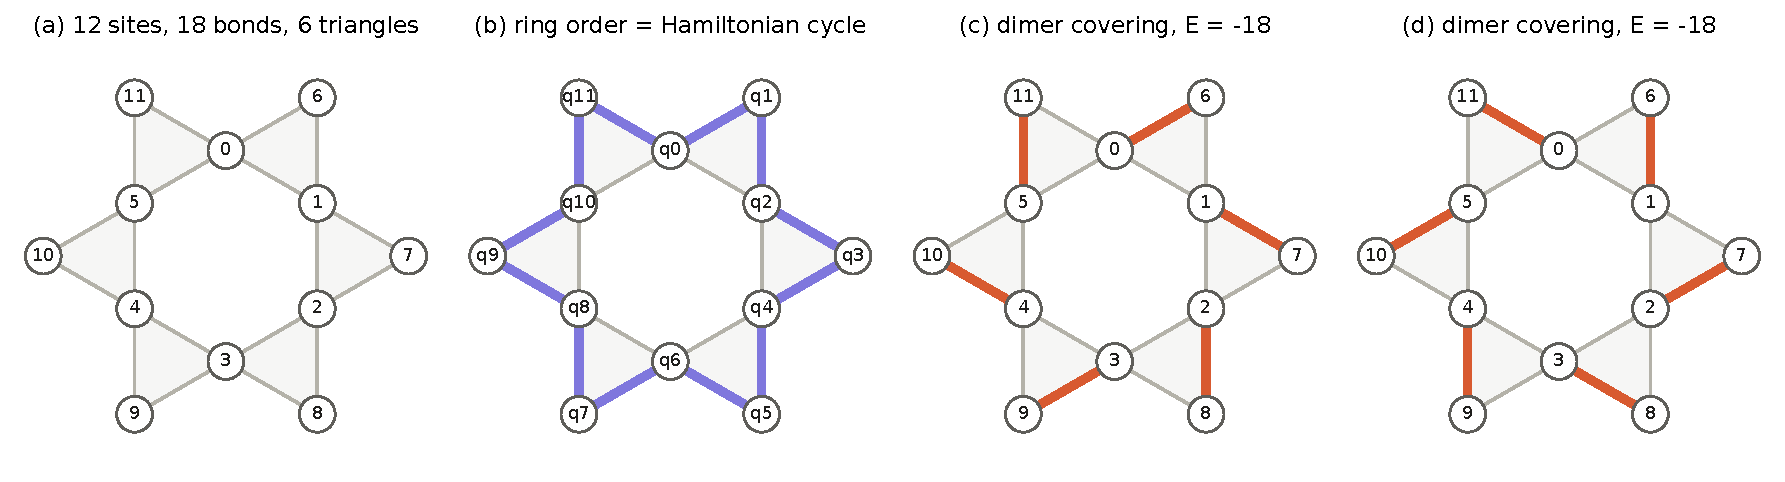
\includegraphics[width=\linewidth]{lattice}
  \caption{(a) The kagome star: hexagon sites 0--5, tips 6--11, six corner-sharing triangles
    (shaded). (b) The ring order used by the ansatzes: qubit $q_k$ hosts site
    $\sigma(k)$ of the Hamiltonian cycle, and the 12 ring bonds (purple) are all lattice bonds.
    (c, d) The two dimer coverings $M_1$ and $M_2$ of \cref{thm:ground}; each places one
    singlet in every triangle, so each has energy $-18$.}
  \label{fig:lattice}
\end{figure}

Figure~\ref{fig:lattice} shows the whole argument: panels (c) and (d) each put one dimer in every
triangle, and panel (b) is their union.

\subsection*{Exercises}

\begin{exer}\label{exer:allup}
  Compute $\bra{0^{12}}H\ket{0^{12}}$ and explain why the all-up state is an eigenstate of $H$.
\end{exer}
\begin{sol}
  On $\ket{00}$, $Z_iZ_j=+1$ and $X_iX_j$, $Y_iY_j$ map $\ket{00}$ to $\pm\ket{11}$ with opposite
  signs ($XX\ket{00}=\ket{11}$, $YY\ket{00}=-\ket{11}$), so $h_{ij}\ket{00}=\ket{00}$. Every one of
  the 18 bonds contributes $+1$: the energy is $+18$. More generally $h=2\SWAP-I$ and $\SWAP$
  fixes $\ket{0^{12}}$, so it is an eigenstate (the maximal-$S^z$ member of the ferromagnetic
  multiplet).
\end{sol}

\begin{exer}
  Compute $\bra{D_{M_1}}h_{ij}\ket{D_{M_1}}$ for a bond $\{i,j\}\notin M_1$, and recover
  $\bra{D_{M_1}}H\ket{D_{M_1}}=-18$ by counting bonds instead of triangles.
\end{exer}
\begin{sol}
  If $\{i,j\}\notin M_1$, sites $i$ and $j$ sit in different singlets, so the state factorises
  across them and $\langle\sigma^a_i\sigma^a_j\rangle=\langle\sigma^a_i\rangle\langle\sigma^a_j\rangle$.
  The reduced state of one half of a singlet is $I/2$, so $\langle\sigma^a\rangle=0$ and the bond
  contributes $0$. The 6 matched bonds contribute $-3$ each (\cref{lem:bond}) and the other 12
  contribute $0$: total $-18$. This counting gives the energy of $\ket{D_{M_1}}$; the triangle
  bound of \cref{thm:ground} is what proves that no state does better.
\end{sol}

\begin{prob}
  Using the loop rule of \cref{prop:overlap}, compute $|\braket{D_{M}}{D_{M'}}|$ for two
  coverings of a 12-site ring whose union consists of three loops of length 4.
\end{prob}
\begin{sol}
  Each loop contributes $2^{1-4/2}=\tfrac12$, so the overlap is $2^{-3}=\tfrac18$. Fewer, longer
  loops mean smaller overlap: $2^{L-N/2}$ with $L$ loops on $N$ sites.
\end{sol}

\section{The circuits and why they fit}
\label{sec:ansatz}

Both ansatzes of the challenge share one skeleton: a singlet product state followed by
two-qubit gates on a ring of qubits. This section defines them, shows that they use the
\emph{same} gate family, and proves the statement the whole benchmark depends on: laid along a
Hamiltonian cycle, both start in the ground space of \cref{thm:ground}.

\subsection{Building blocks}

\begin{dfn}[Singlet preparation]\label{dfn:singlet}
  \py{singlet_pair(a, b)} applies $X_a X_b$, then $H_a$, then $\mathrm{CX}_{a\to b}$:
  \[
    \begin{quantikz}[row sep=0.25cm, column sep=0.3cm]
      \lstick{$\ket0_a$} & \gate{X} & \gate{H} & \ctrl{1} & \qw \\
      \lstick{$\ket0_b$} & \gate{X} & \qw      & \targ{}  & \qw
    \end{quantikz}
    \;=\;\ket{s}_{ab}.
  \]
\end{dfn}

Indeed $\ket{00}\mapsto\ket{11}\mapsto\tfrac{1}{\sqrt2}(\ket0-\ket1)\ket1\mapsto
\tfrac1{\sqrt2}(\ket{01}-\ket{10})$. It costs one CX per pair, six in total.

\begin{dfn}[eSWAP]\label{dfn:eswap}
  For $\phi\in\RR$, $\eSWAP(\phi)=\exp(-i\tfrac\phi2\SWAP)$ on two qubits.
\end{dfn}

\begin{lem}[eSWAP is a Heisenberg bond evolution]\label{lem:eswap}
  \[
    \eSWAP(\phi)=e^{-i\phi/4}\,R_{XX}(\tfrac\phi2)R_{YY}(\tfrac\phi2)R_{ZZ}(\tfrac\phi2)
    =e^{-i\phi/4}\exp\!\bigl(-i\tfrac\phi4\,h\bigr),
  \]
  where $R_{PP}(\theta)=\exp(-i\tfrac\theta2 P\otimes P)$ and $h=XX+YY+ZZ$. Moreover
  $\eSWAP(0)=I$ and $\eSWAP(\pi)=-i\,\SWAP$.
\end{lem}

\begin{proof}
  By \cref{lem:bond}, $\SWAP=\tfrac12(I+h)$, so
  $\exp(-i\tfrac\phi2\SWAP)=e^{-i\phi/4}\exp(-i\tfrac\phi4 h)$. The three terms of $h$
  commute (they are simultaneously diagonal in the Bell basis), so the exponential factorises
  into $R_{XX}(\phi/2)R_{YY}(\phi/2)R_{ZZ}(\phi/2)$. $\SWAP$ has eigenvalues $\pm1$, hence
  $\exp(-i\tfrac\pi2\SWAP)$ multiplies the $+1$ eigenspace by $-i$ and the $-1$ eigenspace by
  $+i$, which is $-i\,\SWAP$.
\end{proof}

\begin{rem}[The paper's eSWAP]
  The 2022 notebook built its eSWAP from $\mathrm{CX}$, $\mathrm{CRX}$, $X$ and $R_Z$.
  Numerically it equals $X_0\cdot\eSWAP(\phi)$ up to a global phase: the stray $X$ means it is
  not the identity at $\phi=0$. The package keeps it for reproduction as
  \py{ansatz.gate = "legacy"} and defaults to the decomposition of \cref{lem:eswap}.
\end{rem}

\subsection{The ring skeleton}

\begin{dfn}[Ring bonds and site order]\label{dfn:ring}
  On $n=12$ qubits arranged in a ring, the \emph{even ring bonds} are
  $\mathcal E=\{(0,1),(2,3),\dots,(10,11)\}$ and the \emph{odd ring bonds} are
  $\mathcal O=\{(11,0),(9,10),\dots,(1,2)\}$ (\py{ring_bonds}). A \emph{site order} is a bijection
  $\sigma:\{0,\dots,11\}\to V$; qubit $q_k$ hosts lattice site $\sigma(k)$, and the Hamiltonian is
  written in qubit labels accordingly (\py{Lattice.site_order}).
\end{dfn}

\begin{dfn}[RVB and HVA]\label{dfn:ansatz}
  Both start from $\ket{D_\mathcal E}=\bigotimes_{(a,b)\in\mathcal E}\ket s_{ab}$. With one layer
  ($\mathrm{reps}=1$),
  \begin{align*}
    \ket{\psi_{\mathrm{RVB}}(\phi)}&=\prod_{k=6}^{11}\eSWAP_{e_k}(\phi_k)\prod_{k=0}^{5}\eSWAP_{o_k}(\phi_k)\,\ket{D_\mathcal E},
      &&\phi\in\RR^{12},\\
    \ket{\psi_{\mathrm{HVA}}(\phi,\gamma)}&=e^{-i\frac\gamma2\Hev}\,e^{-i\frac\phi2\Hod}\,\ket{D_\mathcal E},
      &&(\phi,\gamma)\in\RR^{2},
  \end{align*}
  where $o_k$, $e_k$ enumerate $\mathcal O$ and $\mathcal E$, and $\Hod=\sum_{b\in\mathcal O}h_b$,
  $\Hev=\sum_{b\in\mathcal E}h_b$. The odd layer acts first.
\end{dfn}

The RVB ansatz follows the symmetry-adapted construction of Seki, Shirakawa and Yunoki
\parencite{seki2020}; the HVA follows Wiersema \emph{et al.}\ \parencite{wiersema2020}.
\Cref{lem:eswap} makes the relation exact: a bond gate of RVB with angle $\phi_k$ is,
up to phase, the HVA bond gate $e^{-i\frac\theta2h}$ with $\theta=\phi_k/2$. \textbf{RVB is HVA
with untied angles.} Both compile to the same circuit structure, which is why they have the same
two-qubit gate count after transpilation (\cref{tab:circuits}). The terms within $\Hod$ commute
(the bonds of $\mathcal O$ are disjoint), and so do those of $\Hev$, so each layer is exact; there is
no Trotter error inside a layer.

\begin{figure}[H]
  \centering
  \begin{subfigure}{0.72\linewidth}
    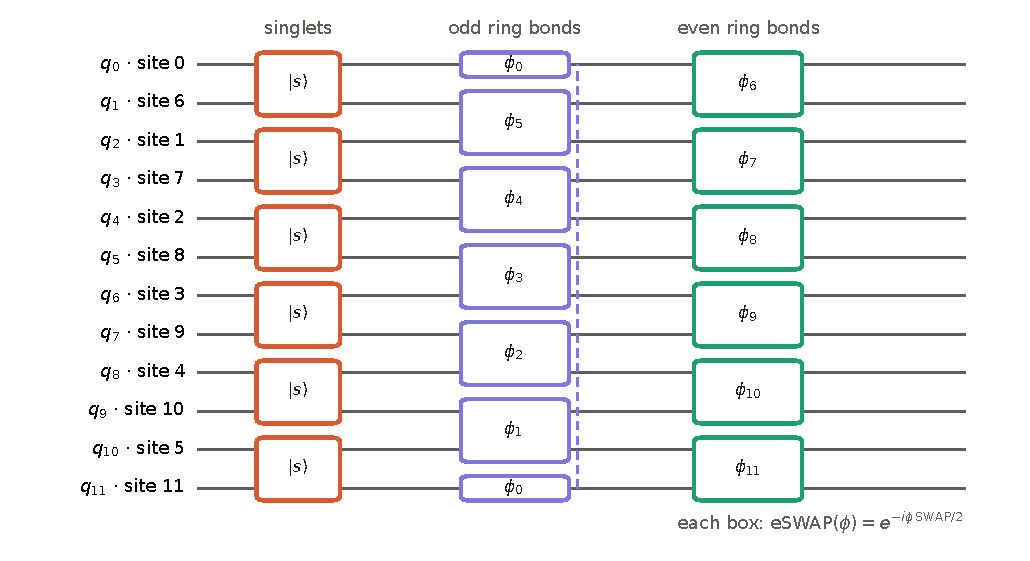
\includegraphics[width=\linewidth]{circuit_rvb}
    \caption{RVB: one angle per bond (12 parameters).}
  \end{subfigure}\\[0.6em]
  \begin{subfigure}{0.72\linewidth}
    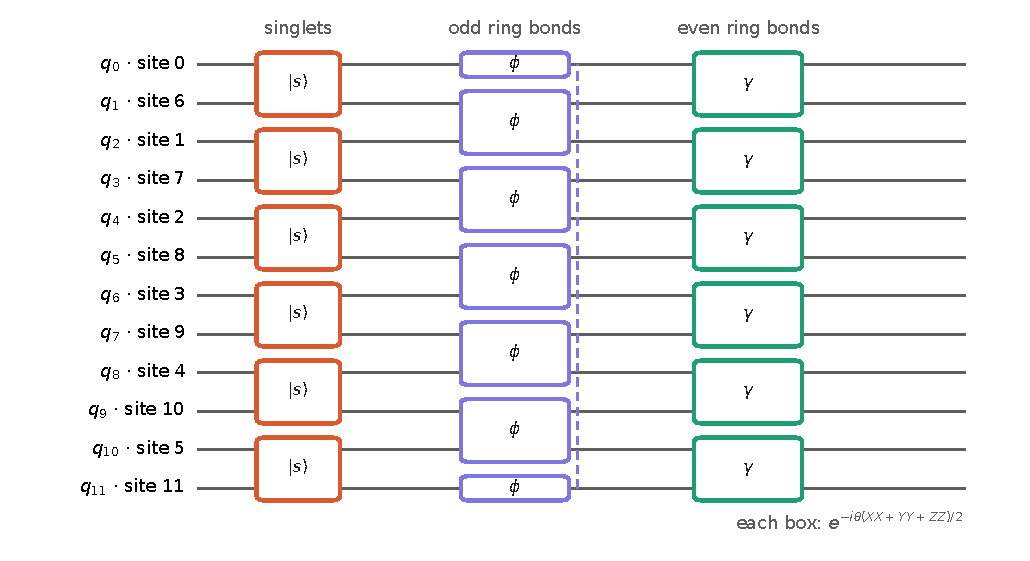
\includegraphics[width=\linewidth]{circuit_hva}
    \caption{HVA: one angle per layer (2 parameters).}
  \end{subfigure}
  \caption{The two ring ansatzes with the default Hamiltonian-cycle site order. Orange: singlet
    preparation on the even ring bonds. Purple: odd-bond layer, including the wrap-around bond
    $(q_{11},q_0)$ drawn as two linked half boxes. Teal: even-bond layer. Every box is the same
    Heisenberg bond evolution; only the parameter sharing differs.}
  \label{fig:circuits}
\end{figure}

\subsection{Why a Hamiltonian cycle}

\begin{thm}*![The ring ansatzes start in the ground space]\label{thm:cycle}
  Let $\sigma$ be the Hamiltonian-cycle order $\sigma=(0,6,1,7,2,8,3,9,4,10,5,11)$. Then
  \begin{enumerate}
    \item the even ring bonds map to the covering $M_1$ and the odd ring bonds to $M_2$;
    \item every ring bond is a lattice bond, and the six hexagon bonds are exactly the lattice
      bonds not on the ring;
    \item $\ket{\psi_{\mathrm{RVB}}(0)}=\ket{\psi_{\mathrm{HVA}}(0,\gamma)}=\ket{D_{M_1}}$ for all
      $\gamma$, with energy $E_0=-18$.
  \end{enumerate}
\end{thm}

\begin{proof}
  (1) $\sigma$ sends $(2k,2k+1)\mapsto\{k,6+k\}\in M_1$ and $(2k-1,2k)\mapsto\{6+k-1,k\}=\{k,6+(k-1)\}\in M_2$,
  including the wrap-around $(11,0)\mapsto\{11,0\}=\{0,6+5\}$. (2) The ring is $M_1\cup M_2$,
  all spokes; the remaining $\VNumBonds-12=6$ bonds are the hexagon. (3) By \cref{lem:eswap}
  $\eSWAP(0)=I$, and $e^{0}=I$, so at $\phi=0$ the state is $\ket{D_\mathcal E}=\ket{D_{M_1}}$ by
  (1). The even layer acts on $\ket{D_{M_1}}$ through bonds $b\in\mathcal E$ that carry its own
  singlets, where $h_b\ket{D_{M_1}}=-3\ket{D_{M_1}}$, so
  $e^{-i\frac\gamma2\Hev}\ket{D_{M_1}}=e^{9i\gamma}\ket{D_{M_1}}$: a global phase. The energy
  is $-18$ by \cref{thm:ground}.
\end{proof}

\begin{prop}[Identity order is hard]\label{prop:identity}
  With $\sigma=\mathrm{id}$, only \VRingFracIdentity{} of the ring bonds and \VSingletIdentity{}
  of the 6 singlet pairs are lattice bonds. Both ansatzes have $E(0)=\VEzeroHvaIdentity$, and the
  global minimum of the HVA energy is $\VHvaMinIdentity$, a relative error of about $40\,\%$
  that no optimiser can remove.
\end{prop}

\begin{proof}
  Identity ring pairs are $\{k,k+1\}$. Lattice bonds among them: the five hexagon bonds
  $\{0,1\},\dots,\{4,5\}$ and $\{11,0\}$, so $6$ of $12$. Of the singlet pairs
  $\{0,1\},\{2,3\},\{4,5\}$ are bonds and $\{6,7\},\{8,9\},\{10,11\}$ are not. At zero
  parameters the state is the singlet product on these pairs: three singlets on bonds give $-9$,
  and every other bond joins two different singlets, contributing $0$ (Exercise in
  \cref{sec:problem}). The minimum is computed in \py{docsgen.physics.hva_minimum} (grid search
  refined by Nelder--Mead on the exact energy); Figure~\ref{fig:landscape} shows the landscape.
\end{proof}

\begin{figure}[H]
  \centering
  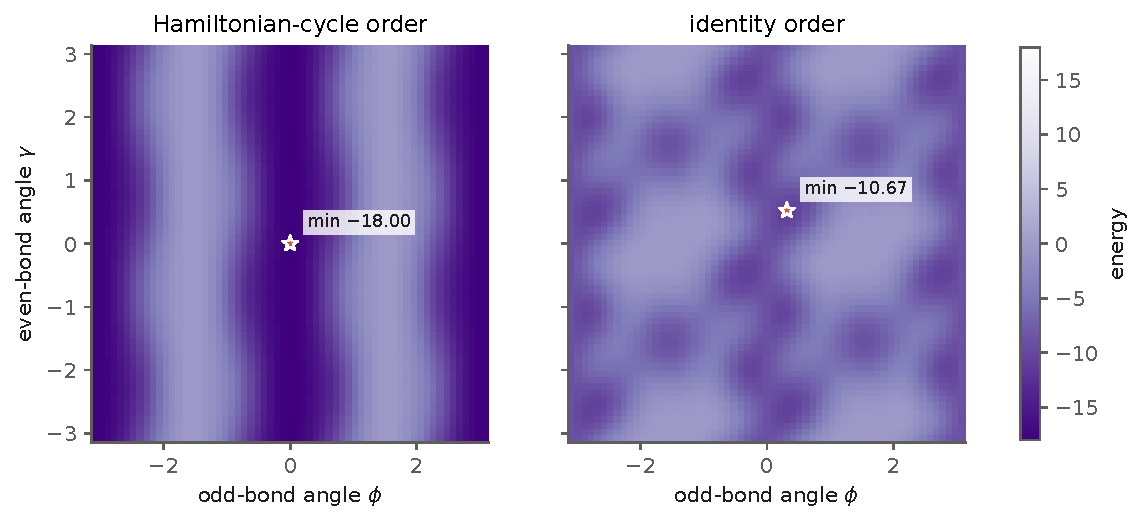
\includegraphics[width=0.86\linewidth]{hva_landscape}
  \caption{Exact HVA energy over $(\phi,\gamma)\in[-\pi,\pi]^2$. Left: Hamiltonian-cycle order.
    The minimum $-18$ is the whole line $\phi=0$ (and $\phi=\pm\pi$, where
    $e^{-i\frac\phi2 h}$ is again trivial up to phase), as \cref{thm:cycle} predicts. Right:
    identity order. The best the ansatz can do is $\VHvaMinIdentity$.}
  \label{fig:landscape}
\end{figure}

Figure~\ref{fig:landscape} is the circuit choice in one picture: the same two-parameter circuit
is exact in one site order and $40\,\%$ off in the other. The minimum on the left is a valley,
not a point, so an optimiser only needs to drive $\phi$ to zero; $\gamma$ is free there.

\begin{rem}[What the 2022 notebook actually did]
  The notebook never transpiled a 12-site Hamiltonian. It hand-wrote a 16-qubit Hamiltonian on
  Guadalupe's physical qubits, whose 12-cycle is the device's heavy-hex loop, and transpiled the
  ring ansatz with an initial layout that is \emph{not} a faithful map of the lattice. Level-3
  routing moved the ring onto the loop anyway, and the V1 \py{Estimator} ignored the circuit
  layout. The result was the Hamiltonian-cycle order by accident. A faithful port with
  \py{observable.apply_layout(layout)} but identity order would silently make the benchmark
  unsolvable (\cref{prop:identity}); this is why \py{site_order} is a first-class, tested
  concept in the package (\py{docs/physics.md}, section~5).
\end{rem}

\begin{rem}[What the circuit does not see]
  Hexagon bonds are never acted on by a gate. That is harmless here, because the ground state
  has no singlets on them, but it makes the ansatz blind to correlations on the hexagon. The
  option \py{ansatz.lattice_aware = true} adds a third HVA sub-layer on those bonds, at the cost of
  routing: kagome contains triangles and heavy-hex does not, so the hexagon bonds can never all be
  physical couplings.
\end{rem}

\subsection*{Exercises}

\begin{exer}
  Show that $e^{-i\frac\phi2 h}$ is trivial up to phase at $\phi=\pi$, and explain the second
  valley at $\phi=\pm\pi$ in Figure~\ref{fig:landscape}.
\end{exer}
\begin{sol}
  $h=2\SWAP-I$, so $e^{-i\frac\pi2h}=e^{i\pi/2}e^{-i\pi\SWAP}$. $\SWAP$ has eigenvalues $\pm1$
  and $e^{\mp i\pi}=-1$, so $e^{-i\pi\SWAP}=-I$. The odd layer is the identity up to phase,
  the state is again $\ket{D_{M_1}}$, and the energy is $-18$ for every $\gamma$.
\end{sol}

\begin{exer}
  How many free parameters does each ansatz have with $\mathrm{reps}=r$ layers, and how many
  bond gates?
\end{exer}
\begin{sol}
  Each layer has 12 bond gates (6 odd, 6 even). RVB: $12r$ parameters; HVA: $2r$ parameters
  ($3r$ with the lattice-aware sub-layer, which adds 6 more gates per layer). Both have $12r$ bond
  gates on the ring.
\end{sol}

\begin{prob}
  Find a site order other than the default for which \cref{thm:cycle} still holds, and
  describe all of them.
\end{prob}
\begin{sol}
  The theorem needs the ring to be a Hamiltonian cycle with the even bonds forming a perfect
  matching. The star has a unique Hamiltonian cycle as an edge set ($M_1\cup M_2$, since a
  Hamiltonian cycle must use both spokes of every degree-2 tip, which is already all 12 spokes).
  Valid orders are its $12$ starting points times $2$ directions. Starting at an odd
  position swaps the roles of $M_1$ and $M_2$, which is equally good by symmetry. So there are 24
  valid site orders, all equivalent.
\end{sol}

\section{The software pipeline}
\label{sec:pipeline}

The package turns one TOML file into one results directory. Each stage is a module with a
single job, so each can be tested and replaced on its own. Table~\ref{tab:pipeline} lists them in
the order a run visits them.

\begin{table}[H]
  \centering
  \small
  \begin{tabular}{L{3.2cm}L{4.6cm}L{7.4cm}}
    \toprule
    stage & module & role \\
    \midrule
    configuration & \py{config.py} & pydantic models for lattice, ansatz, optimiser, backend; validated TOML in \py{configs/} \\
    lattice & \py{lattice.py} & immutable bond list and \py{site_order} (\cref{dfn:ring}), independent of Qiskit \\
    Hamiltonian & \py{hamiltonian.py} & \py{SparsePauliOp} of \cref{dfn:ham}; exact reference by sparse Lanczos \\
    ansatz & \py{ansatz/} & \py{RVBAnsatz}, \py{HVAnsatz}, library baselines; \py{unshare.py} for parameter shift (\cref{sec:m1}) \\
    compilation & \py{transpile.py} & preset pass manager (level 3), \py{initial_layout} on the heavy-hex loop, \py{observable.apply_layout} \\
    estimation & \py{estimators.py} & exact statevector, sampled Aer (ideal or noisy), IBM Runtime; one protocol \py{EnergyEstimator} \\
    optimisation & \py{optimizers/} & in-repo ADAM, SPSA, gradient descent; gradient strategies (forward, central, SPSA, parameter shift) \\
    driver & \py{vqe.py} & objective with trace, ideal-energy tracking, final re-measurement \\
    persistence & \py{results.py} & \py{results/<UTC>-<name>/}: config, result, traces, environment, log \\
    \bottomrule
  \end{tabular}
  \caption{Pipeline stages of \texttt{kagome-vqe} (\py{src/kagome_vqe/}).}
  \label{tab:pipeline}
\end{table}

\subsection{Compilation for the device}

The target is \py{FakeGuadalupeV2}, Qiskit's snapshot of the 16-qubit \texttt{ibmq\_guadalupe}
including its calibrated noise. Its coupling map is heavy-hex, with a 12-qubit loop
$(1,2,3,5,8,11,14,13,12,10,7,4)$ (\py{GUADALUPE_HEAVY_HEX_LOOP}). Passing this loop as the initial
layout puts every ring bond on a physical coupling, so the ring gates need no routing SWAPs. The
observable then follows the circuit through \py{apply_layout}; this is the explicit Qiskit~2
replacement for the accident described in \cref{sec:ansatz}.

\begin{table}[H]
  \centering
  % Generated by `uv run python -m docsgen`; do not edit.
\begin{tabular}{lcccccc}
\toprule
ansatz & parameters & gate occurrences & PS energies & CX (Guadalupe) & CX (unshared) & depth \\
\midrule
HVA & \VParamsHva & $2\times 18$ & \VPsEnergiesHva & \VCxHva & \VCxHvaUnshared & \VDepthHva \\
RVB & \VParamsRvb & $12$ & \VPsEnergiesRvb & \VCxRvb & \VCxRvbUnshared & \VDepthRvb \\
\bottomrule
\end{tabular}

  \caption{Circuit cost on \py{FakeGuadalupeV2} (optimisation level 3, heavy-hex loop layout).
    ``PS energies'' is the number of energies one parameter-shift gradient needs
    (\cref{sec:m1}). ``Unshared'' is the circuit with one parameter per gate occurrence,
    which parameter shift requires; it has the same two-qubit cost.}
  \label{tab:circuits}
\end{table}

Both ansatzes cost \VCxHva{} CX after transpilation, and the count does not depend on the
layout hint (\VCxRvbNoLayout{} for RVB without it), so routing is not the cause. The count
decomposes as $6+12\times5$: six singlet CX and five CX for each of the 12 Heisenberg bond
gates. A general two-qubit unitary needs at most three CX, so the bond gates are not being
resynthesised.

\begin{prop}[Binding parameters before transpiling]\label{prop:bound}
  The circuits are transpiled once with \emph{unbound} parameters. Level-3 two-qubit
  resynthesis (block consolidation followed by unitary synthesis) needs numeric matrices and
  skips parametric gates, so each $R_{ZZ}R_{YY}R_{XX}$ block keeps its naive decomposition
  minus cancellations. Binding the parameters first gives $\VBoundCxHva=6+12\times3$ CX (depth
  \VBoundDepthHva{} instead of \VDepthHva{} for HVA). At $\theta_k=\VBoundTheta$ for every
  parameter, under the full \py{FakeGuadalupeV2} noise model, the fraction of the exact energy
  that survives rises from \VParamKeepHva{} to \VBoundKeepHva{} (HVA) and from \VParamKeepRvb{}
  to \VBoundKeepRvb{} (RVB).
\end{prop}

\begin{proof}
  Measured, not derived: \py{docsgen.physics.bound_compilation} transpiles both versions with
  the same layout and seed and evaluates each with \VNoiseShots{} shots per basis. The CX
  counts are the transpiler's output. The comparison uses $\theta\neq0$ because at zero the
  bound circuit collapses to the 6-CX singlet preparation, which would be a trivial win
  (\cref{rem:easy}).
\end{proof}

\begin{rem}[Consequence for the roadmap]
  Re-transpiling for every parameter vector costs classical time for each energy (seconds, at
  level 3), which matters for parameter shift with \VPsEnergiesHva{} energies per step. Two cheaper
  routes give the same 3-CX blocks: transpile the bond gate once as the textbook 3-CX
  decomposition of $\exp(-i(aXX+bYY+cZZ))$ with parametric single-qubit rotations, or bind and
  transpile only the 12 distinct two-qubit blocks. Either one is the first, nearly free step of
  roadmap M4 (depth compression), and it should raise the noisy floor before any approximate
  method is tried.
\end{rem}

\begin{rem}[A stale figure in the prose docs]
  Until \texttt{687d0ae}, \py{docs/physics.md} (section~8) said the transpiled circuits have
  ``66 (HVA) to 93 (RVB)'' CX, a sentence from the initial commit \texttt{d4a05ac}. With the
  current code RVB compiles to \VCxRvb{} CX with or without the layout (\cref{tab:circuits}),
  equal to HVA, as \cref{lem:eswap} predicts; the legacy eSWAP gives 54. The corrected text
  gives 66 for both and attributes 93 to the 2022 notebook's layout; see \cref{sec:status}.
\end{rem}

\subsection{Estimating an energy}

The Hamiltonian splits into three groups of qubit-wise commuting terms (all $XX$, all $YY$, all
$ZZ$), so one energy costs \VMeasGroups{} measured circuits. With $s$ shots per basis, the
estimator returns the sampled mean of each Pauli term and their weighted sum. Throughout,
``shots per energy'' means shots per measurement basis, and ``shots spent'' counts all bases.

\begin{dfn}[Relative error]
  For an energy $E$ and the exact $E_0$, $\varepsilon(E)=|E-E_0|/|E_0|$ (\py{relative_error}).
  The challenge asked for $\varepsilon<1\,\%$.
\end{dfn}

The package distinguishes three energies of a run, and the distinction matters from M0 on:
\begin{itemize}
  \item the \emph{trace} energies, one per evaluation the optimiser asked for (noisy, finite shots);
  \item the \emph{final} energy: the final parameters re-measured once with a large, fixed budget
    (\py{backend.final_shots}, 16384 per basis);
  \item the \emph{ideal} energy: the exact statevector energy of the current parameters, recorded
    after every iteration but never shown to the optimiser (\py{track_ideal_energy}). It measures
    how good the \emph{parameters} are, separately from the noise floor.
\end{itemize}

\section{What device noise does to the energy}
\label{sec:noise}

On a noisy device the circuit prepares a mixed state $\rho$ instead of $\ket{\psi(\theta)}$, and
the measured energy is $\operatorname{Tr}(\rho H)$. This section explains why that energy sits on
a plateau far above $-18$ even at the exact parameters, and why the plateau is nearly a constant
\emph{factor} times the ideal energy. That structure decides which improvements can work.

\begin{prop}[Variational principle for mixed states]\label{prop:mixed}
  For every density matrix $\rho$, $\operatorname{Tr}(\rho H)\ge E_0$.
\end{prop}

\begin{proof}
  Write $\rho=\sum_k p_k\ket{\chi_k}\bra{\chi_k}$ with $p_k\ge0$, $\sum p_k=1$. Each
  $\bra{\chi_k}H\ket{\chi_k}\ge E_0$, and a convex combination of numbers $\ge E_0$ is $\ge E_0$.
\end{proof}

Hence a noisy reading \emph{below} $-18$ cannot come from a physical state; it signals sampling
fluctuation or an over-corrected mitigation, never a better answer.

\begin{prop}[Depolarising noise rescales the energy]\label{prop:depol}
  Let $\mathcal D_p(\rho)=(1-p)\rho+p\,I/2^{n}$. Then $\operatorname{Tr}(\mathcal D_p(\rho)H)=(1-p)\operatorname{Tr}(\rho H)$.
  If each qubit's readout flips independently with probability $q$, every two-qubit Pauli
  expectation is multiplied by $(1-2q)^2$, so the measured energy is $(1-2q)^2\operatorname{Tr}(\rho H)$.
\end{prop}

\begin{proof}
  $\operatorname{Tr}(H)=0$ because every term of $H$ is a non-identity Pauli string, so the
  maximally mixed part contributes nothing. For readout, a $\pm1$ outcome flipped with
  probability $q$ has mean $(1-2q)$ times the true mean, and the two outcomes of a $ZZ$-type term
  flip independently, giving $(1-2q)^2$. The same holds in the $X$ and $Y$ bases, where the
  measurement is a $Z$ measurement after a basis rotation.
\end{proof}

Real device noise is neither global nor uniform, but if it were, the two factors would simply
multiply. Table~\ref{tab:floor} tests that by switching the noise channels of the
\py{FakeGuadalupeV2} model on one at a time, at the exact parameters, with \VNoiseShots{} shots
per basis.

\begin{table}[H]
  \centering
  % Generated by `uv run python -m docsgen`; do not edit.
\begin{tabular}{lccccc}
\toprule
ansatz & noise-free & readout only & gate + $T_1/T_2$ only & full & $E_0\, r_{\mathrm{ro}}\, r_{\mathrm{g}}$ \\
\midrule
HVA & \VFloorHvaIdeal & \VFloorHvaReadout & \VFloorHvaGate & \VFloorHvaFull & \VKeepHvaProduct \\
RVB & \VFloorRvbIdeal & \VFloorRvbReadout & \VFloorRvbGate & \VFloorRvbFull & \VKeepRvbProduct \\
\bottomrule
\end{tabular}

  \caption{Energy at the exact parameters (all zero) on \py{FakeGuadalupeV2}, transpiled to
    \VCxHva{} CX. Readout error alone retains $r_{\mathrm{ro}}=\VKeepHvaReadout$ of the energy;
    gate and $T_1/T_2$ errors alone retain $r_{\mathrm g}=\VKeepHvaGate$ (HVA). The last
    column multiplies the two factors and nearly matches the full model.}
  \label{tab:floor}
\end{table}

\begin{figure}[H]
  \centering
  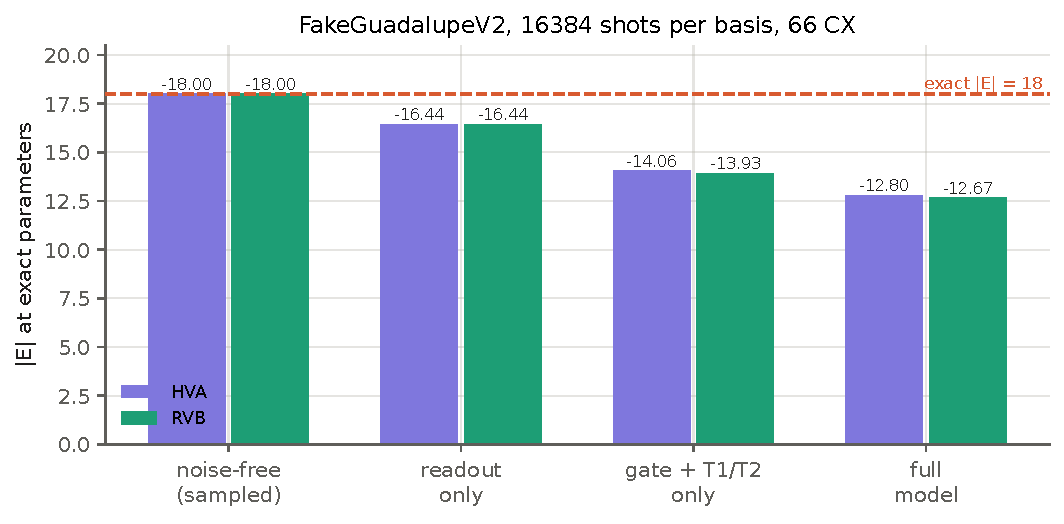
\includegraphics[width=0.75\linewidth]{noise_floor}
  \caption{The same data. The noisy energy is not a convergence failure: the exact optimum
    itself reads \VFloorHvaFull{} (HVA) under the full model. The near-multiplicative structure
    (readout $\times$ gate $\approx$ full) is what makes rescaling-type mitigation promising.}
  \label{fig:floor}
\end{figure}

\begin{prop}[Zero shot noise at the exact optimum]\label{prop:zerovar}
  In each of the three measurement bases, every shot taken on $\ket{D_{M_1}}$ returns the same
  value $-6$ for that basis's part of $H$. The sampled energy is exactly $-18$ with zero variance,
  for any number of shots.
\end{prop}

\begin{proof}
  Take the $Z$ basis; $X$ and $Y$ are identical because a singlet is anticorrelated along every
  axis. A shot returns $z\in\{\pm1\}^{12}$ with $z_i=-z_{6+i}$ on every dimer
  $\{i,6+i\}\in M_1$. The $ZZ$ part of $H$ evaluates to
  \[
    \sum_{i=0}^{5}z_iz_{6+i}+\sum_{i=0}^{5}\bigl(z_iz_{i+1}+z_{i+1}z_{6+i}\bigr)
    =-6+\sum_{i=0}^{5}\bigl(z_iz_{i+1}-z_{i+1}z_{i}\bigr)=-6,
  \]
  grouping the 12 unmatched bonds by triangle: in $\tau_i$, the hexagon bond and the second spoke
  share site $i+1$ and see $z_i$ and $z_{6+i}=-z_i$ respectively.
\end{proof}

\Cref{prop:zerovar} has a practical side. The real spread of sampled energies falls towards
zero as the parameters approach the optimum: \VSpreadLowReal{} at the start point
$(\phi,\gamma)=(\pi/4,\pi/4)$ with 1024 shots, \VSpreadLowZero{} at the optimum. The primitive's
reported standard error is a state-independent bound (\cref{sec:m0}) and does not show this.
Noise-free sampled runs therefore become \emph{easier} as they converge; with device noise the
mixed state breaks the cancellation and the shot noise stays.

\subsection*{Exercises}

\begin{exer}
  Using \cref{prop:depol} and Table~\ref{tab:floor}, estimate the uniform readout flip
  probability $q$ that would explain the readout-only energy of HVA.
\end{exer}
\begin{sol}
  $(1-2q)^2=\VKeepHvaReadout$, so $1-2q\approx0.956$ and $q\approx2.2\,\%$, a typical readout
  error for that device generation.
\end{sol}

\begin{exer}
  Why does \cref{prop:zerovar} not contradict the fact that the individual terms $X_iX_j$ on
  unmatched bonds have nonzero variance on $\ket{D_{M_1}}$?
\end{exer}
\begin{sol}
  The terms are random individually, but within a triangle the two unmatched terms are
  perfectly anticorrelated, shot by shot, so their sum is deterministic. Variance of a sum
  includes covariances, which cancel the individual variances here.
\end{sol}

\section{Milestone M0: honest noisy simulation}
\label{sec:m0}

\begin{tcolorbox}[colback=gray!5, colframe=gray!40, title={M0 at a glance}, fonttitle=\bfseries]
  \textbf{Question.} Are the noisy numbers real?\quad
  \textbf{Answer.} They were not: the simulator never sampled. After M0 the noisy floor is
  \VPostFinalMin{} to \VPostFinalMax{} (was about $-14$).\\
  \textbf{Code.} Commit \texttt{0433fd7}. \textbf{Results.} \py{results/statevector_m0-summary},
  \py{results/fake_guadalupe_m0-summary}. \textbf{Status.} Done; hardware check H0 deferred.
\end{tcolorbox}

\subsection{Goal and exit criteria}

The first noisy benchmark reported energies around $-14$ on \py{FakeGuadalupeV2}. While
diagnosing that plateau (\cref{sec:noise}), three defects in the simulation turned up. M0 had to
remove them before any method comparison could be trusted. Its exit criterion was a new noisy
baseline in the README, backed by four checks: the standard error falls as $1/\sqrt{\text{shots}}$,
identical parameter rows differ between calls, readout error alone moves the energy, and
RVB\,+\,ADAM no longer climbs.

\subsection{The three defects}

\begin{enumerate}
  \item \textbf{No sampling.} The \py{aer_ideal} and \py{aer_noisy} backends used Aer's own
    \py{EstimatorV2}, which computes expectation values with \py{save_expectation_value}
    instead of sampling. Shots had no effect, reported standard errors were zero, and readout
    error was never applied. A unit test meant to check shot noise passed vacuously.
  \item \textbf{Seed reuse made a fake gradient.} Each row of a parameter batch got a fixed
    simulator seed. Identical parameters then gave different energies per row, with the
    \emph{same} pattern on every call: a spread of \VSeedBugSpread{} across \VSeedBugRows{}
    identical rows. With finite-difference step $\varepsilon=\VFdEps$ this is a constant fake
    gradient of about \VSeedBugGrad{} per component, and ADAM followed it.
  \item \textbf{``Best energy'' was biased low.} Reporting the minimum over a noisy trace
    selects favourable fluctuations.
\end{enumerate}

The second item explains the most visible symptom, RVB\,+\,ADAM climbing from
\VPreBestRvbAdam{} to \VPreFinalRvbAdam{} (Figure~\ref{fig:m0}, right panel). SPSA was unaffected
because its random perturbation directions average a fixed per-row bias away.\footnote{The
numbers in item~2 are quoted from \py{docs/roadmap.md}, section~1.3; the code that produced
them was replaced in M0 and cannot be rerun.}

\subsection{Implementation}

\begin{itemize}
  \item \textbf{Sampling estimator.} \py{AerEnergy} now wraps
    \py{qiskit.primitives.BackendEstimatorV2} around an \py{AerSimulator} (density matrix with
    noise, statevector without). Each energy measures the \VMeasGroups{} commuting bases with the
    requested shots, so shot noise and readout error appear as on hardware.
  \item \textbf{Fresh seeds.} Every call draws a new simulator seed from the run's generator
    (\py{_next_seed}). Runs stay reproducible from the run seed, but repeated parameters no
    longer share a noise pattern.
  \item \textbf{Final re-measurement.} \py{run_vqe} re-measures the final parameters once with
    \py{backend.final_shots} (16384 per basis) and reports that as \emph{the} result; the trace
    minimum is kept only as a diagnostic.
\end{itemize}

\subsection{Results}

\begin{table}[H]
  \centering
  % Generated by `uv run python -m docsgen`; do not edit.
\begin{tabular}{lccccc}
\toprule
 & \multicolumn{2}{c}{before M0 (no sampling)} & \multicolumn{3}{c}{after M0 (sampled, re-measured)} \\
\cmidrule(lr){2-3}\cmidrule(lr){4-6}
combination & final & best of trace & final & best of trace & rel.\ error \\
\midrule
RVB + SPSA & \VPreFinalRvbSpsa & \VPreBestRvbSpsa & \VPostFinalRvbSpsa & \VPostBestRvbSpsa & \VPostErrRvbSpsa \\
RVB + ADAM & \VPreFinalRvbAdam & \VPreBestRvbAdam & \VPostFinalRvbAdam & \VPostBestRvbAdam & \VPostErrRvbAdam \\
HVA + SPSA & \VPreFinalHvaSpsa & \VPreBestHvaSpsa & \VPostFinalHvaSpsa & \VPostBestHvaSpsa & \VPostErrHvaSpsa \\
HVA + ADAM & \VPreFinalHvaAdam & \VPreBestHvaAdam & \VPostFinalHvaAdam & \VPostBestHvaAdam & \VPostErrHvaAdam \\
\bottomrule
\end{tabular}

  \caption{The noisy FakeGuadalupeV2 benchmark (the paper's four combinations) before and after
    M0. ``Final'' after M0 is the re-measured energy. All four now sit on the noise floor of
    \cref{sec:noise}; before M0 the floor looked higher because readout error was missing.}
  \label{tab:m0}
\end{table}

\begin{figure}[H]
  \centering
  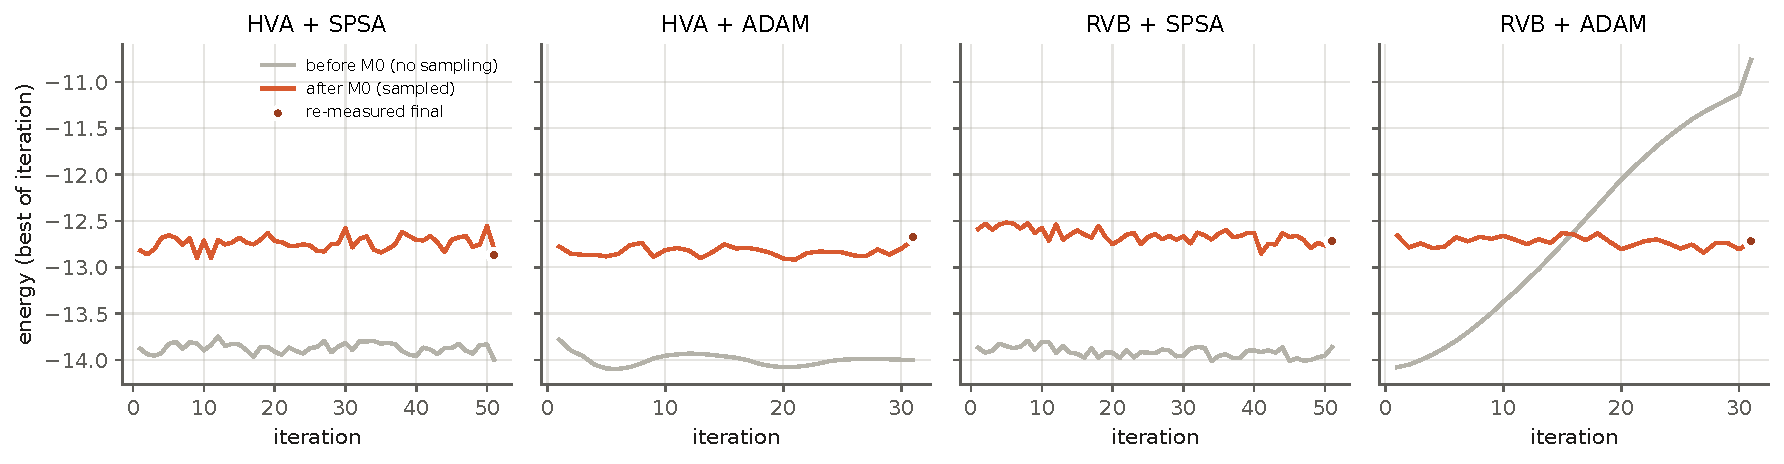
\includegraphics[width=\linewidth]{m0_before_after}
  \caption{Convergence before (grey) and after (orange) M0, best energy of each iteration. The
    upward shift of about one unit (from about $-14$ to $-12.8$) is the readout error that was
    missing: it adds bias. The climb of
    RVB\,+\,ADAM (right) is gone. Dots: the re-measured final energy.}
  \label{fig:m0}
\end{figure}

Figure~\ref{fig:m0} and Table~\ref{tab:m0} show the two effects of M0 separately. The
\emph{level} moved from about $-14$ to about $-12.8$: that is readout error, consistent with the
factor \VKeepHvaReadout{} of Table~\ref{tab:floor}. The \emph{shape} of RVB\,+\,ADAM changed from
a steady climb to a flat line: that is the fake gradient disappearing. On the exact
statevector backend nothing changed (Table~\ref{tab:m0sv}), as expected, since none of the three
defects touches exact simulation.

\begin{table}[H]
  \centering
  % Generated by `uv run python -m docsgen`; do not edit.
\begin{tabular}{lcc}
\toprule
combination & final energy & rel.\ error \\
\midrule
RVB + SPSA & \VSvFinalRvbSpsa & \VSvErrRvbSpsa \\
RVB + ADAM & \VSvFinalRvbAdam & \VSvErrRvbAdam \\
HVA + SPSA & \VSvFinalHvaSpsa & \VSvErrHvaSpsa \\
HVA + ADAM & \VSvFinalHvaAdam & \VSvErrHvaAdam \\
\bottomrule
\end{tabular}

  \caption{Exact statevector benchmark, for reference. HVA returns to zero parameters exactly;
    RVB with SPSA stops at \VSvErrRvbSpsa.}
  \label{tab:m0sv}
\end{table}

\subsection{Checks}

\begin{itemize}
  \item \emph{Standard error falls as $1/\sqrt{\text{shots}}$.} Over \VSpreadRepeats{} repeats at
    the start point, the real spread is \VSpreadLowReal{} at 1024 shots and \VSpreadHighReal{} at
    4096: a factor of two for four times the shots.
  \item \emph{Identical rows differ between calls; readout alone moves the energy}
    ($-18\to\VFloorHvaReadout$). Both are unit-tested in the package.
  \item \emph{RVB\,+\,ADAM no longer climbs}: final \VPostFinalRvbAdam.
\end{itemize}

\subsection{Findings carried forward}

\begin{rem}[The reported standard error is a bound]\label{rem:stdbound}
  The sampling primitive reports $\sum_i|c_i|\,\sigma_i/\sqrt{s}$ over the Pauli terms, which
  ignores correlations between terms. At the start point it reports \VSpreadLowReported{} at
  1024 shots against a real spread of \VSpreadLowReal{}, about \VSpreadRatio{} times too large;
  at the optimum the real spread without noise is exactly zero (\cref{prop:zerovar}). Method comparisons in M1
  and later therefore use repeated runs, never the reported \py{std}.
\end{rem}

\begin{rem}[Simulation cost]
  Noisy density-matrix simulation costs about \VSecPerEnergy{}\,s per energy regardless of the
  shot count (the density matrix is evolved once, sampling is cheap). Simulator studies can use
  large shot budgets for free; hardware cannot. This is what limited the noisy part of M1 to one
  seed and to RVB.
\end{rem}

\subsection{Problems solved and open}

\begin{itemize}
  \item[\checkmark] The three defects are fixed and covered by unit tests; the vacuous Aer test
    now asserts real shot noise.
  \item[\checkmark] New noisy baseline in the README (Table~\ref{tab:m0}).
  \item[$\circ$] \textbf{Hardware checkpoint H0 deferred} at the group's request. The IBM
    Runtime code path is kept and tested in local mode only, so the fake-backend floor is not yet
    calibrated against a real device.
\end{itemize}

\section{Milestone M1: better gradients}
\label{sec:m1}

\begin{tcolorbox}[colback=gray!5, colframe=gray!40, title={M1 at a glance}, fonttitle=\bfseries]
  \textbf{Question.} Which gradient gives the most precision per shot?\quad
  \textbf{Answer.} RVB: ADAM with parameter shift (\VMIdealRvbPs{} without gate noise,
  \VMNoisyRvbPs{} with it). HVA: plain SPSA (\VMIdealHvaSpsa).\\
  \textbf{Code.} Commit \texttt{1a27c28}. \textbf{Results.} \py{results/m1_ideal-summary},
  \py{results/m1_noisy-summary}. \textbf{Status.} Done; three follow-ups open.
\end{tcolorbox}

\subsection{Goal and exit criteria}

The paper's ADAM runs used forward finite differences with step $\varepsilon=\VFdEps$. Under
shot noise such a difference divides noise by $\varepsilon$. M1 added an exact gradient
(parameter shift) and a two-energy hybrid, then compared all of them at an \emph{equal shot
budget}. Exit: a recommended default gradient per ansatz, recorded in the configs.

\subsection{Theory}

\begin{thm}[Parameter-shift rule \parencite{mitarai2018,schuld2019}]\label{thm:ps}
  Let $U(\theta)=e^{-i\theta G}$ with $G$ Hermitian, $G^2=\tfrac14 I$ (eigenvalues
  $\pm\tfrac12$), and $f(\theta)=\bra{\psi}V^\dagger U(\theta)^\dagger W^\dagger A\,W U(\theta)V\ket\psi$
  for fixed unitaries $V$, $W$ and an observable $A$. Then for every $\theta$,
  \[
    f'(\theta)=\tfrac12\bigl[f(\theta+\tfrac\pi2)-f(\theta-\tfrac\pi2)\bigr].
  \]
\end{thm}

\begin{proof}
  Because $(2G)^2=I$, $U(\theta)=\cos\tfrac\theta2\,I-i\sin\tfrac\theta2\,(2G)$. Substituting,
  $f$ is a quadratic form in $(\cos\frac\theta2,\sin\frac\theta2)$, hence a trigonometric
  polynomial of degree one: $f(\theta)=a+b\cos\theta+c\sin\theta$ for constants $a,b,c$. Then
  $f(\theta\pm\tfrac\pi2)=a\mp b\sin\theta\pm c\cos\theta$, and the half-difference is
  $-b\sin\theta+c\cos\theta=f'(\theta)$.
\end{proof}

Both ansatzes qualify gate by gate. Each eSWAP is $e^{-i\phi\,\SWAP/2}$, and $G=\SWAP/2$ has
eigenvalues $\pm\frac12$. Each HVA rotation $R_{PP}(\theta)=e^{-i\theta\,PP/2}$ has $G=PP/2$.
The legacy eSWAP contains a controlled rotation, whose generator has three eigenvalues; it
would need a four-term rule and is not supported.

\begin{cor}[Shared parameters]\label{cor:shared}
  If a parameter $\theta_j$ drives $K_j$ such gates, then
  $\partial_{\theta_j}E=\sum_{k=1}^{K_j}\tfrac12\bigl[E(\varphi+\tfrac\pi2e_k)-E(\varphi-\tfrac\pi2e_k)\bigr]$
  evaluated at the \emph{unshared} vector $\varphi=\mathrm{expand}(\theta)$, which has one entry
  per occurrence. One gradient costs $2\sum_jK_j$ energies: $\VPsEnergiesRvb$ for RVB ($K_j=1$)
  and $\VPsEnergiesHva$ for HVA ($K_j=18$).
\end{cor}

\begin{proof}
  The energy is $E(\theta)=F(\mathrm{expand}(\theta))$ where $F$ treats occurrences as
  independent. By the chain rule, $\partial_{\theta_j}E=\sum_{k:\,k\mapsto j}\partial_{\varphi_k}F$,
  and each term is given by \cref{thm:ps} with $V,W$ the rest of the circuit.
\end{proof}

A single shift of a shared HVA parameter does \emph{not} work: the summed generator
$\sum_kG_k$ has many eigenvalues, so $E$ is a higher-degree trigonometric polynomial in
$\theta_j$. The package implements \cref{cor:shared} with \py{unshare_parameters}, which rewrites
the circuit with one parameter per occurrence and returns a \py{ParameterMap} with
\py{expand} ($\theta\mapsto\varphi$) and \py{contract} (sum of occurrence gradients). The
unshared circuit prepares the same state and transpiles to the same \VCxHvaUnshared{} CX
(Table~\ref{tab:circuits}).

\begin{prop}[Gradient noise per component]\label{prop:gradnoise}
  Suppose every energy estimate carries independent noise of standard deviation $\sigma$. The
  per-component noise of the gradient estimate is
  \[
    \text{forward: }\frac{\sqrt2\,\sigma}{\varepsilon},\qquad
    \text{central: }\frac{\sqrt2\,\sigma}{2\varepsilon},\qquad
    \text{parameter shift: }\sigma\sqrt{K_j/2}.
  \]
  At an equal budget $B$ of shots per iteration split over $m$ energies, $\sigma=\sigma_B\sqrt m$,
  where $\sigma_B$ is the noise of one energy measured with all $B$ shots.
\end{prop}

\begin{proof}
  Forward: $(\hat E(\theta+\varepsilon e_j)-\hat E(\theta))/\varepsilon$ has variance
  $2\sigma^2/\varepsilon^2$. Central: $(\hat E_+-\hat E_-)/(2\varepsilon)$ has variance
  $2\sigma^2/(4\varepsilon^2)$. Parameter shift: a sum of $K_j$ half-differences, each with variance
  $2\sigma^2/4$, gives $K_j\sigma^2/2$. Shot noise scales as $1/\sqrt{\text{shots}}$, and each
  of the $m$ energies gets $B/m$ shots, so $\sigma=\sigma_B\sqrt m$.
\end{proof}

With $\varepsilon=\VFdEps$ the forward difference amplifies noise \VSigmaFwd-fold at fixed shots
per energy, while parameter shift gives \VSigmaPsRvb$\sigma$ for RVB. At equal budget
(Table~\ref{tab:m1}) the picture sharpens: for RVB parameter shift wins by an order of magnitude
(\VBudgetPsRvb$\sigma_B$ against \VBudgetFwdRvb$\sigma_B$), but for HVA its 72 energies cancel the
advantage (\VBudgetPsHva$\sigma_B$ against \VBudgetFwdHva$\sigma_B$). Finite differences are
also biased, by $O(\varepsilon)$ for forward and $O(\varepsilon^2)$ for central; parameter shift is
unbiased.

\begin{dfn}[SPSA and the hybrid]
  SPSA \parencite{spall1992} draws a random sign vector $\Delta\in\{\pm1\}^n$ and estimates
  $\hat g=\Delta\,[E(\theta+c\Delta)-E(\theta-c\Delta)]/(2c)$ from two energies, whatever $n$.
  \emph{Plain SPSA} takes the step $\theta\leftarrow\theta-a\,\hat g$ with a \VSpsaCalibrated{}
  gain $a=\VSpsaLr$ in M1. The \emph{hybrid} feeds the same two-energy estimate into ADAM
  \parencite{kingma2014}, whose step $-\eta\,\hat m/(\sqrt{\hat v}+\epsilon)$ divides the averaged
  gradient $\hat m$ by its running root-mean-square $\sqrt{\hat v}$.
\end{dfn}

\subsection{Protocol}

Every method spends the same \VMBudget{} shots per measurement basis per iteration, split evenly
over the $m$ energies its gradient needs. All gradient methods share ADAM with learning rate
$\VAdamLr$, so differences come from the gradients alone; plain SPSA is the baseline. The metric
is the \emph{ideal} energy of the final parameters (\cref{sec:pipeline}): how good the parameters
are, separately from the noise floor. Two settings:
\begin{itemize}
  \item shot noise only (\py{aer_ideal}), \VMItersHva{} iterations, \VMSeeds{} seeds, both
    ansatzes (\py{configs/m1_gradients_ideal.toml});
  \item full \py{FakeGuadalupeV2} noise, \VMNoisyIters{} iterations, one seed, RVB only, because
    noisy simulation costs about \VSecPerEnergy{}\,s per energy and HVA parameter shift needs 72
    energies per step (\py{configs/m1_gradients_noisy.toml}).
\end{itemize}

\subsection{Results}

\begin{table}[H]
  \centering
  \footnotesize
  \setlength{\tabcolsep}{4pt}
  % Generated by `uv run python -m docsgen`; do not edit.
\begin{tabular}{llccccc}
\toprule
 &  &  & \multicolumn{2}{c}{gradient noise per component} & \multicolumn{2}{c}{noise-free error of final parameters} \\
\cmidrule(lr){4-5}\cmidrule(lr){6-7}
ansatz & method & $m$ & fixed shots ($\sigma$) & equal budget ($\sigma_B$) & shot noise (\VMSeeds{} seeds) & device noise (1 seed) \\
\midrule
HVA & ADAM, forward differences (paper) & \VMEnergiesHvaFwd & \VSigmaFwd & \VBudgetFwdHva & \VMIdealHvaFwd ${}\pm{}$ \VMIdealHvaFwdSd & not run \\
 & ADAM, central differences & \VMEnergiesHvaCen & \VSigmaCen & \VBudgetCenHva & \VMIdealHvaCen ${}\pm{}$ \VMIdealHvaCenSd & not run \\
 & ADAM, SPSA gradient (hybrid) & \VMEnergiesHvaHyb & -- & -- & \VMIdealHvaHyb ${}\pm{}$ \VMIdealHvaHybSd & not run \\
 & ADAM, parameter shift & \VMEnergiesHvaPs & \VSigmaPsHva & \VBudgetPsHva & \VMIdealHvaPs ${}\pm{}$ \VMIdealHvaPsSd & not run \\
 & plain SPSA & \VMEnergiesHvaSpsa & -- & -- & \VMIdealHvaSpsa ${}\pm{}$ \VMIdealHvaSpsaSd & not run \\
\midrule
RVB & ADAM, forward differences (paper) & \VMEnergiesRvbFwd & \VSigmaFwd & \VBudgetFwdRvb & \VMIdealRvbFwd ${}\pm{}$ \VMIdealRvbFwdSd & \VMNoisyRvbFwd \\
 & ADAM, central differences & \VMEnergiesRvbCen & \VSigmaCen & \VBudgetCenRvb & \VMIdealRvbCen ${}\pm{}$ \VMIdealRvbCenSd & not run \\
 & ADAM, SPSA gradient (hybrid) & \VMEnergiesRvbHyb & -- & -- & \VMIdealRvbHyb ${}\pm{}$ \VMIdealRvbHybSd & \VMNoisyRvbHyb \\
 & ADAM, parameter shift & \VMEnergiesRvbPs & \VSigmaPsRvb & \VBudgetPsRvb & \VMIdealRvbPs ${}\pm{}$ \VMIdealRvbPsSd & \VMNoisyRvbPs \\
 & plain SPSA & \VMEnergiesRvbSpsa & -- & -- & \VMIdealRvbSpsa ${}\pm{}$ \VMIdealRvbSpsaSd & \VMNoisyRvbSpsa \\
\bottomrule
\end{tabular}

  \caption{Equal-budget gradient comparison. $m$: energies per iteration, read from the
    evaluation counts of the runs. Gradient noise from \cref{prop:gradnoise}. Errors are the
    noise-free relative error of the final parameters: mean $\pm$ sample standard deviation
    over seeds.\protect\footnotemark}
  \label{tab:m1}
\end{table}
\footnotetext{Sample standard deviation ($\mathrm{ddof}=1$). The README's M1 table originally used
the population value ($\mathrm{ddof}=0$), smaller by $\sqrt{4/5}$ for five seeds; \py{main} switched it to the sample value in
\texttt{687d0ae}. The means agree, and \py{docsgen/tests} checks them.}

\begin{figure}[H]
  \centering
  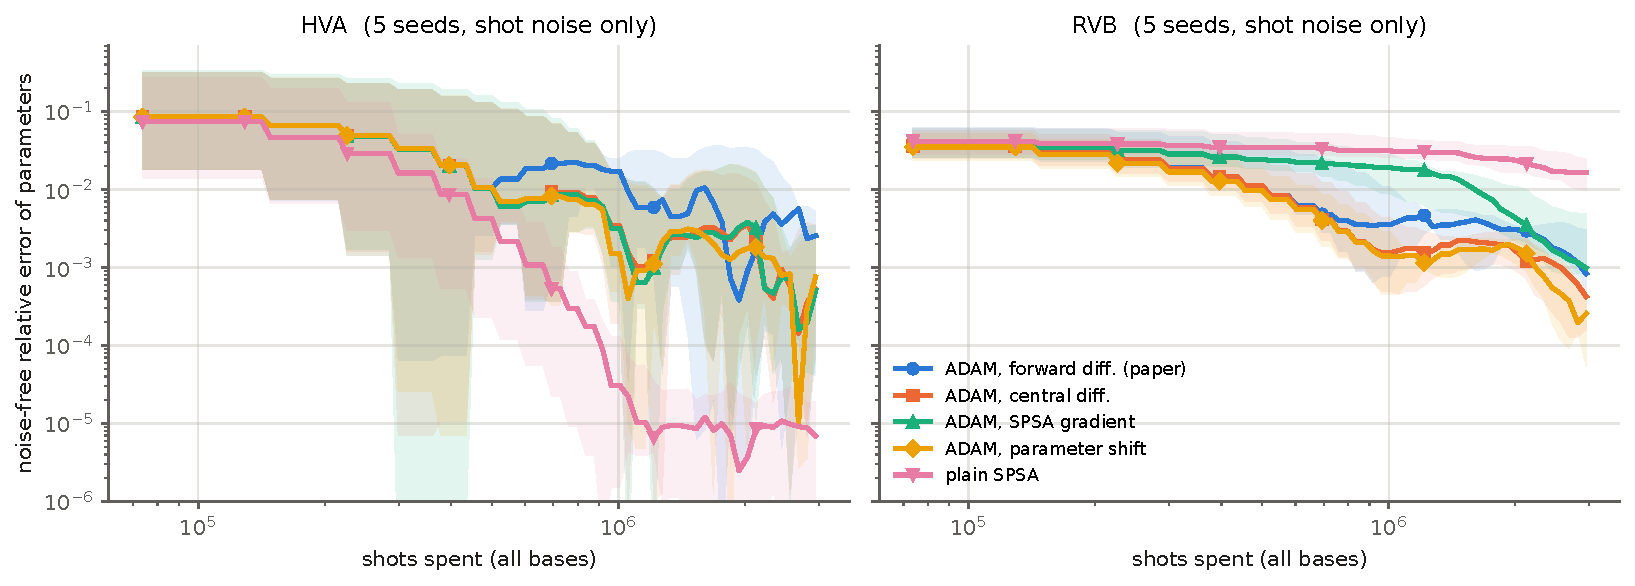
\includegraphics[width=\linewidth]{m1_ideal_vs_shots}
  \caption{Noise-free relative error of the current parameters against shots spent (all bases),
    shot noise only. Line: median over seeds; band: min--max. The same metric as
    \py{kagome_vqe.plotting.plot_ideal_vs_shots}, coloured by method consistently across this
    report and the slides.}
  \label{fig:m1curves}
\end{figure}

\begin{figure}[H]
  \centering
  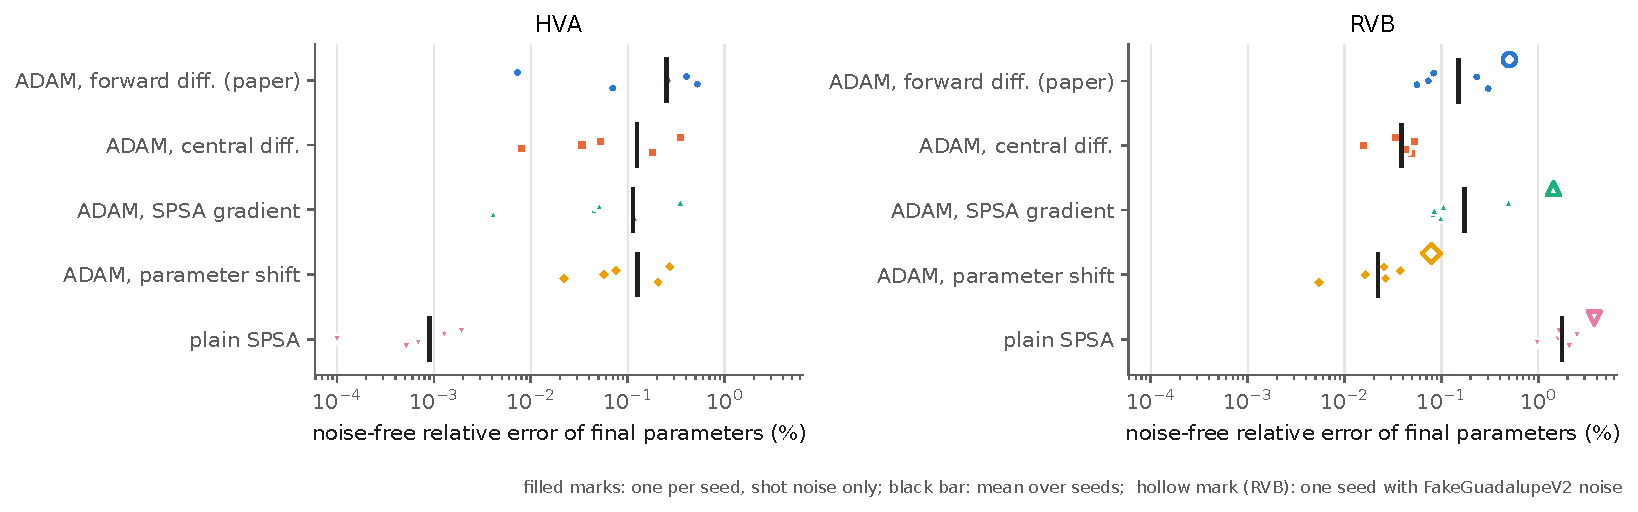
\includegraphics[width=\linewidth]{m1_final}
  \caption{Final noise-free error per method. Filled marks: one per seed (shot noise only); black
    bar: mean. Hollow marks (RVB): the single seed with device noise.}
  \label{fig:m1final}
\end{figure}

Figures~\ref{fig:m1curves} and~\ref{fig:m1final} support three readings.
\begin{enumerate}
  \item \textbf{RVB: parameter shift is best} with and without device noise
    (\VMIdealRvbPs{} and \VMNoisyRvbPs{}), against \VMIdealRvbFwd{} and \VMNoisyRvbFwd{} for the
    paper's forward differences. This matches \cref{prop:gradnoise}: at equal budget its
    per-component noise is an order of magnitude lower. Plain SPSA is the least precise for RVB's
    12 parameters (\VMIdealRvbSpsa), and its two-energy estimate is a poor direction in 12
    dimensions.
  \item \textbf{HVA: plain SPSA is best} by two orders of magnitude (\VMIdealHvaSpsa), while
    every ADAM variant, \emph{whatever its gradient}, ends near $0.1\,\%$. Identical plateaus
    for gradients of very different quality point to the update rule, not the gradient. Near the
    minimum the true gradient vanishes but the noise does not, so $\sqrt{\hat v}$ tracks the noise
    and ADAM's normalised step stays of order $\eta=\VAdamLr$ per component: it keeps jittering
    around the minimum. Plain SPSA's step $a\hat g$ shrinks in mean with the gradient. HVA has
    only two parameters, so SPSA's random directions lose little.
  \item \textbf{Noise floor unchanged.} The re-measured noisy energies of the M1 runs stay at the
    floor of \cref{sec:noise} (\VMNoisyFinalRvbPs{} for parameter shift): better gradients
    improve the parameters, not what the device reads.
\end{enumerate}

\subsection{Problems solved and open}

\begin{itemize}
  \item[\checkmark] Parameter shift matches finite differences without noise to about
    $10^{-9}$ for HVA, RVB and \py{real_amplitudes}; energy counts 24 and 72 are unit-tested.
  \item[\checkmark] Defaults recorded: \py{configs/fake_guadalupe_rvb_adam_ps.toml} (RVB, ADAM +
    parameter shift) and \py{configs/ibm_hva_spsa.toml} (HVA, SPSA).
  \item[$\circ$] \textbf{ADAM's step size limits HVA.} A decaying learning rate should be tried
    before concluding that SPSA is intrinsically better for HVA.
  \item[$\circ$] \textbf{RVB had not converged} when the budget ran out
    (Figure~\ref{fig:m1curves}, right: curves still falling at three million shots); longer runs
    may reorder the close finishers.
  \item[$\circ$] \textbf{The noisy check used one seed.} Repeat with more seeds before relying on
    the smaller differences (e.g.\ forward against central).
\end{itemize}

\subsection*{Exercises}

\begin{exer}
  With $\varepsilon=0.1$, how many times more shots per energy does a forward difference need to
  match the per-component noise of parameter shift on RVB?
\end{exer}
\begin{sol}
  Equate $\sqrt2\sigma_1/0.1=\sigma_2/\sqrt2$: $\sigma_1/\sigma_2=0.05$, so $1/0.05^2=400$ times
  more shots per energy. With 13 instead of 24 energies per gradient, the total shot cost is still
  about $400\times13/24\approx217$ times higher.
\end{sol}

\begin{exer}
  Show that a single symmetric shift of a shared HVA parameter, $\tfrac12[E(\theta_j+\tfrac\pi2)-E(\theta_j-\tfrac\pi2)]$,
  is \emph{not} the derivative in general.
\end{exer}
\begin{sol}
  With $K$ gates sharing $\theta_j$, $E$ is a trigonometric polynomial of degree up to $K$ in
  $\theta_j$ (each gate contributes degree one). The two-term rule is exact only for degree one;
  for example $E=\cos2\theta$ gives $\tfrac12[\cos(2\theta+\pi)-\cos(2\theta-\pi)]=0\neq-2\sin2\theta$.
\end{sol}

\section{Milestone M2: error mitigation}
\label{sec:m2}

\begin{tcolorbox}[colback=gray!5, colframe=gray!40, title={M2 at a glance}, fonttitle=\bfseries]
  \textbf{Question.} How much of the noise bias can mitigation remove?\quad
  \textbf{Answer so far.} On \py{FakeGuadalupeV2}, readout correction plus total-spin symmetry
  filtering appeared to bring the HVA bias at the exact parameters from \VMtHvaZeroRawRel{} to
  \VMtHvaZeroRoSymRel{} at no extra shots per energy. This report found that the small residual
  is an over-correction of \VMxOverPct{} cancelling the residual noise (\cref{sec:m2cancel}); treating readout consistently
  leaves \VMxHvaZeroFullCtfRel.\\
  \textbf{Code.} Commit \texttt{c9272e3}; results recorded in \texttt{e87051a}; estimator
  corrected in \texttt{56aadd3}. \textbf{Results.} \py{results/m2-evaluation-0},
  \py{results/m2-evaluation-0p3}, \py{results/m2_vqe-summary}. \textbf{Status.}
  \emph{Reopened}: the chosen stack is withdrawn and reruns are in progress; H1 skipped.
\end{tcolorbox}

\subsection{Goal and exit criteria}

After M0 the noisy energy is an honest estimate, but it sits \VMtHvaZeroRawRel{} above the truth at
the exact parameters (\cref{sec:noise}). An optimiser cannot remove that bias
(\cref{prop:mixed}); mitigation can try. M2 implemented four techniques as composable estimator
layers, measured each combination at \emph{fixed} parameters where the noise-free energy is
known, and chose a stack for full optimisations and later hardware runs. Exit: a measured bias
and shot cost for every stack, and a chosen stack.

\subsection{Theory}

All four techniques act on the energy estimator, not on the circuit's parameters. Two of them
need the individual shots, so they replace the Estimator primitive with a sampler that measures
the \VMeasGroups{} bases itself. Since every term of $H$ is $X_iX_j$, $Y_iY_j$ or $Z_iZ_j$, the
three qubit-wise commuting groups are the uniform bases: all qubits measured in $X$, all in $Y$,
or all in $Z$.

\begin{ntn}
  For one basis, a shot is a bit string $b\in\{0,1\}^{n}$, $n=\VNumSites$, and the noise-free
  outcome distribution is $p(b)$. Qubit $q$'s readout flips $0\to1$ with probability $e_0^{(q)}$
  and $1\to0$ with probability $e_1^{(q)}$, independently of the other qubits; its confusion
  matrix is
  $A_q=\bigl(\begin{smallmatrix}1-e_0^{(q)} & e_1^{(q)}\\ e_0^{(q)} & 1-e_1^{(q)}\end{smallmatrix}\bigr)$,
  with columns indexed by the prepared bit and rows by the read bit. A Pauli term $P_t$ of the
  measured basis acts on the support $S_t$, and $s(b)=(-1)^{b}$ is the eigenvalue of bit $b$.
\end{ntn}

\begin{dfn}[Counts-level energy estimator]\label{dfn:counts}
  Given weights $w_q\colon\{0,1\}\to\RR$, a shot $b$ contributes
  $\varepsilon(b)=\sum_t c_t\prod_{q\in S_t}w_q(b_q)$ and the energy estimate is the mean of
  $\varepsilon$ over the shots, summed over the three bases. Without readout correction
  $w_q=s$. With readout correction $w_q=v_q$, where $v_q=(1,-1)\,A_q^{-1}$, that is
  \[
    v_q(0)=\frac{1-e_1^{(q)}+e_0^{(q)}}{1-e_0^{(q)}-e_1^{(q)}},\qquad
    v_q(1)=-\frac{1+e_1^{(q)}-e_0^{(q)}}{1-e_0^{(q)}-e_1^{(q)}} .
  \]
  \emph{Symmetry filtering} discards every shot whose Hamming weight $|b|$ differs from $n/2$
  before the mean is taken.
\end{dfn}

Because $\varepsilon$ is computed per shot, the standard error of the mean is the exact one,
$\operatorname{std}(\varepsilon)/\sqrt{\text{shots}}$, instead of the primitive's upper bound
of \cref{rem:stdbound}.

\begin{prop}[Readout correction is unbiased]\label{prop:readout}
  If the readout errors are independent with confusion matrices $A_q$ and the $v_q$ use the same
  $A_q$, then for every Pauli term $\mathbb E\bigl[\prod_{q\in S_t}v_q(\tilde b_q)\bigr]=\langle P_t\rangle$,
  where $\tilde b$ is the read string and $\langle P_t\rangle$ the noise-free expectation.
\end{prop}

\begin{proof}
  Condition on the prepared string $b$. The read bits are independent with
  $\Pr(\tilde b_q=r\mid b_q)=(A_q)_{r b_q}$, so
  $\mathbb E[v_q(\tilde b_q)\mid b_q]=\sum_r v_q(r)(A_q)_{r b_q}=\bigl((1,-1)A_q^{-1}A_q\bigr)_{b_q}=s(b_q)$.
  Independence turns the expectation of the product over $S_t$ into the product of these
  conditional means, $\prod_{q\in S_t}s(b_q)$, which is the eigenvalue of $P_t$ on $b$. Averaging
  over $b\sim p$ gives $\langle P_t\rangle$.
\end{proof}

The price is variance: $|v_q|\approx1/(1-2e)$, so each two-body term's per-shot magnitude grows
by about $1/(1-2e)^2$. With the calibrated mean flip probability $e=\VMtReadoutErr$ (largest
\VMtReadoutErrMax) this is under $10\,\%$.

\begin{prop}[Ring-ansatz states lie in the zero-magnetisation sector of every basis]\label{prop:sector}
  For every parameter value, the RVB and HVA states $\ket{\psi(\theta)}$ of \cref{dfn:ansatz}
  are total-spin singlets, $\vec S_{\mathrm{tot}}^{\,2}\ket{\psi(\theta)}=0$ with
  $\vec S_{\mathrm{tot}}=\sum_i\vec\sigma_i/2$. Consequently, in each uniform basis $X$, $Y$ or
  $Z$, a noise-free shot has exactly $n/2$ ones.
\end{prop}

\begin{proof}
  The initial state is a product of singlets (\cref{dfn:singlet}), each with total spin $0$, so
  the product has $\vec S_{\mathrm{tot}}^{\,2}=0$. Every later gate is generated by
  $\SWAP_{ij}=\tfrac12(I+X_iX_j+Y_iY_j+Z_iZ_j)$ or by $h_{ij}$, both functions of
  $\vec\sigma_i\cdot\vec\sigma_j$, which commutes with every component of $\vec S_{\mathrm{tot}}$.
  Hence each gate commutes with $\vec S_{\mathrm{tot}}^{\,2}$ and the state stays a singlet.
  Now $0=\bra\psi\vec S_{\mathrm{tot}}^{\,2}\ket\psi=\sum_{\alpha}\lVert S^\alpha_{\mathrm{tot}}\ket\psi\rVert^2$,
  so $S^\alpha_{\mathrm{tot}}\ket\psi=0$ for $\alpha=x,y,z$. Measuring every qubit in basis
  $\alpha$ measures the $\sigma^\alpha_i$, and $S^\alpha_{\mathrm{tot}}=\tfrac12(n-2|b|)$ on outcome
  $b$; only $|b|=n/2$ has nonzero amplitude.
\end{proof}

A shot of any other weight was corrupted by noise and can be discarded \parencite{bonetmonroig2018,mcardle2019}.
This is not free: the filter keeps only about \VMtKept{} of the shots under full device noise,
so the shot noise per energy grows by about $\sqrt2$. It also only detects errors that change
the weight; an error that maps the state to another weight-$n/2$ string passes.

\begin{dfn}[Zero-noise extrapolation by local folding]\label{dfn:zne}
  For an odd scale $\lambda=2k+1$, replace every two-qubit gate $G$ of the transpiled circuit by
  $G(G^\dagger G)^k$ \parencite{giurgicatiron2020}. The unitary is unchanged and the two-qubit
  error is amplified roughly $\lambda$-fold. Measure $E(\lambda)$ at $\lambda=1,3,5$ and fit
  $E(\lambda)=A\,e^{-b\lambda}$ \parencite{endo2018}; report $A=E(0)$.
\end{dfn}

The exponential model is the one suggested by \cref{prop:depol}: if each folded gate multiplied
the energy by a fixed factor, $E(\lambda)$ would decay geometrically in $\lambda$. ZNE triples
the shots per energy.

\begin{dfn}[Twin-circuit rescaling]\label{dfn:twin}
  Choose \emph{twin} parameters $\theta_{\mathrm{t}}$ whose noise-free energy
  $E_{\mathrm{ideal}}(\theta_{\mathrm{t}})$ is computable classically, measure the twin once with
  noise, and report $E_{\mathrm{mit}}(\theta)=E_{\mathrm{noisy}}(\theta)\,
  E_{\mathrm{ideal}}(\theta_{\mathrm{t}})/E_{\mathrm{noisy}}(\theta_{\mathrm{t}})$
  \parencite{urbanek2021}. The package picks the twin on a grid of multiples of $\pi/4$ with the
  largest $|E_{\mathrm{ideal}}|$, excluding ground states so the test is not circular.
\end{dfn}

\begin{rem}[When rescaling is exact]
  Under global depolarising noise of the same strength for both circuits, \cref{prop:depol} gives
  $E_{\mathrm{noisy}}=(1-p)E_{\mathrm{ideal}}$ for target and twin alike, and the ratio cancels
  $(1-p)$ exactly. Rescaling therefore works to the extent that the damping factor
  $E_{\mathrm{noisy}}/E_{\mathrm{ideal}}$ is the same for the twin and the target. Nothing
  guarantees that for real noise, which is neither global nor state-independent.
\end{rem}

\subsection{Implementation}

\begin{itemize}
  \item \textbf{Counts layer} (\py{CountsEnergy} in \py{mitigation/counts.py}): measures the three
    bases itself, with Qiskit's backend sampler over Aer (fresh seed per call, as in M0) or the runtime
    \py{SamplerV2}. Readout is calibrated once per estimator by preparing all-zeros and all-ones
    (2 circuits of 16384 shots). In \texttt{c9272e3}, which produced every result in this chapter,
    shots are \emph{filtered first} when both are enabled, then the kept shots are weighted with
    $v_q$. Since \texttt{56aadd3} the order is reversed (\cref{sec:m2cancel}).
  \item \textbf{ZNE} (\py{ZneEnergy}): folds the ISA circuit with
    \py{transpile.fold_two_qubit_gates} once per scale and wraps one inner estimator per scale, so
    readout calibration is repeated per scale. Only the single-qubit measurement suffix is
    translated after folding; re-optimising would cancel the inserted $G^\dagger G$ pairs.
  \item \textbf{Twin} (\py{TwinRescaledEnergy}, \py{choose_twin}): measures the twin once at
    16384 shots per basis when the estimator opens and propagates its uncertainty.
  \item \textbf{Composition}: \py{make_estimator} builds counts processing innermost, then ZNE,
    then rescaling, from a \py{[mitigation]} table in the run config.
  \item \textbf{Evaluation mode}: \py{kagome-vqe benchmark CONFIG --point P --repeats R}
    estimates the energy $R$ times at all parameters equal to $P$, with fresh seeds, and writes
    \py{evaluation.json} with the mean, the real spread, the bias against the noise-free energy,
    the shot cost and a \py{below_ground} flag for means more than two standard errors below
    $E_0$.
\end{itemize}

\subsection{Results at fixed parameters}

Every stack was evaluated \VMtRepeatsZero{} times at two points: the exact parameters
($\theta=0$, noise-free $-18$) and the generic point $\theta=\VBoundTheta$ for every parameter,
where the noise-free energies are \VMtIdealHvaPt{} (HVA) and \VMtIdealRvbPt{} (RVB). Each
energy uses \VMtShots{} circuit shots (4096 per basis), \VMtShotsZne{} with ZNE.

\begin{table}[H]
  \centering
  \footnotesize
  \setlength{\tabcolsep}{4pt}
  \begin{adjustbox}{max width=\linewidth}
    % Generated by `uv run python -m docsgen`; do not edit.
\begin{tabular}{lccccrr}
\toprule
 & \multicolumn{2}{c}{HVA} & \multicolumn{2}{c}{RVB} &  &  \\
\cmidrule(lr){2-3}\cmidrule(lr){4-5}
stack & $\theta=0$ (\VMtIdealHvaZero) & $\theta=\VBoundTheta$ (\VMtIdealHvaPt) & $\theta=0$ (\VMtIdealRvbZero) & $\theta=\VBoundTheta$ (\VMtIdealRvbPt) & shots / energy & one-off shots \\
\midrule
none & \VMtHvaZeroRaw\,{\small(\VMtHvaZeroRawRel)} & \VMtHvaPtRaw\,{\small(\VMtHvaPtRawRel)} & \VMtRvbZeroRaw\,{\small(\VMtRvbZeroRawRel)} & \VMtRvbPtRaw\,{\small(\VMtRvbPtRawRel)} & \VMtShots & 0 \\
readout & \VMtHvaZeroRo\,{\small(\VMtHvaZeroRoRel)} & \VMtHvaPtRo\,{\small(\VMtHvaPtRoRel)} & \VMtRvbZeroRo\,{\small(\VMtRvbZeroRoRel)} & \VMtRvbPtRo\,{\small(\VMtRvbPtRoRel)} & \VMtShots & \VMtSetupRo \\
symmetry & \VMtHvaZeroSym\,{\small(\VMtHvaZeroSymRel)} & \VMtHvaPtSym\,{\small(\VMtHvaPtSymRel)} & \VMtRvbZeroSym\,{\small(\VMtRvbZeroSymRel)} & \VMtRvbPtSym\,{\small(\VMtRvbPtSymRel)} & \VMtShots & 0 \\
readout + symmetry & \VMtHvaZeroRoSym$^\dagger$\,{\small(\VMtHvaZeroRoSymRel)} & \VMtHvaPtRoSym\,{\small(\VMtHvaPtRoSymRel)} & \VMtRvbZeroRoSym\,{\small(\VMtRvbZeroRoSymRel)} & \VMtRvbPtRoSym\,{\small(\VMtRvbPtRoSymRel)} & \VMtShots & \VMtSetupRo \\
\midrule
ZNE & \VMtHvaZeroZne\,{\small(\VMtHvaZeroZneRel)} & \VMtHvaPtZne\,{\small(\VMtHvaPtZneRel)} & \VMtRvbZeroZne\,{\small(\VMtRvbZeroZneRel)} & \VMtRvbPtZne\,{\small(\VMtRvbPtZneRel)} & \VMtShotsZne & 0 \\
readout + ZNE & \VMtHvaZeroRoZne\,{\small(\VMtHvaZeroRoZneRel)} & \VMtHvaPtRoZne\,{\small(\VMtHvaPtRoZneRel)} & \VMtRvbZeroRoZne\,{\small(\VMtRvbZeroRoZneRel)} & \VMtRvbPtRoZne\,{\small(\VMtRvbPtRoZneRel)} & \VMtShotsZne & \VMtSetupRoZne \\
readout + symmetry + ZNE & \VMtHvaZeroRoSymZne$^\dagger$\,{\small(\VMtHvaZeroRoSymZneRel)} & \VMtHvaPtRoSymZne$^\dagger$\,{\small(\VMtHvaPtRoSymZneRel)} & \VMtRvbZeroRoSymZne$^\dagger$\,{\small(\VMtRvbZeroRoSymZneRel)} & \VMtRvbPtRoSymZne$^\dagger$\,{\small(\VMtRvbPtRoSymZneRel)} & \VMtShotsZne & \VMtSetupRoZne \\
\midrule
twin & \VMtHvaZeroTwin$^\dagger$\,{\small(\VMtHvaZeroTwinRel)} & \VMtHvaPtTwin\,{\small(\VMtHvaPtTwinRel)} & \VMtRvbZeroTwin\,{\small(\VMtRvbZeroTwinRel)} & \VMtRvbPtTwin\,{\small(\VMtRvbPtTwinRel)} & \VMtShots & \VMtSetupTwin \\
readout + twin & \VMtHvaZeroRoTwin$^\dagger$\,{\small(\VMtHvaZeroRoTwinRel)} & \VMtHvaPtRoTwin\,{\small(\VMtHvaPtRoTwinRel)} & \VMtRvbZeroRoTwin$^\dagger$\,{\small(\VMtRvbZeroRoTwinRel)} & \VMtRvbPtRoTwin\,{\small(\VMtRvbPtRoTwinRel)} & \VMtShots & \VMtSetupRoTwin \\
readout + symmetry + twin & \VMtHvaZeroRoSymTwin\,{\small(\VMtHvaZeroRoSymTwinRel)} & \VMtHvaPtRoSymTwin\,{\small(\VMtHvaPtRoSymTwinRel)} & \VMtRvbZeroRoSymTwin\,{\small(\VMtRvbZeroRoSymTwinRel)} & \VMtRvbPtRoSymTwin\,{\small(\VMtRvbPtRoSymTwinRel)} & \VMtShots & \VMtSetupRoTwin \\
\bottomrule
\end{tabular}

  \end{adjustbox}
  \caption{Mean energy of \VMtRepeatsZero{} repeats per stack, with the relative bias
    $(\bar E-E_{\mathrm{ideal}})/|E_{\mathrm{ideal}}|$ in brackets; negative means below the
    noise-free value. $^\dagger$: mean more than two standard errors below $-18$, impossible for
    a physical state (\cref{prop:mixed}). The spread between repeats is
    \VMtHvaZeroSymSpread{} to \VMtHvaZeroRoZneSpread{}. One-off shots are the readout
    calibration (per ZNE scale) and the twin measurement.}
  \label{tab:m2}
\end{table}

\begin{figure}[H]
  \centering
  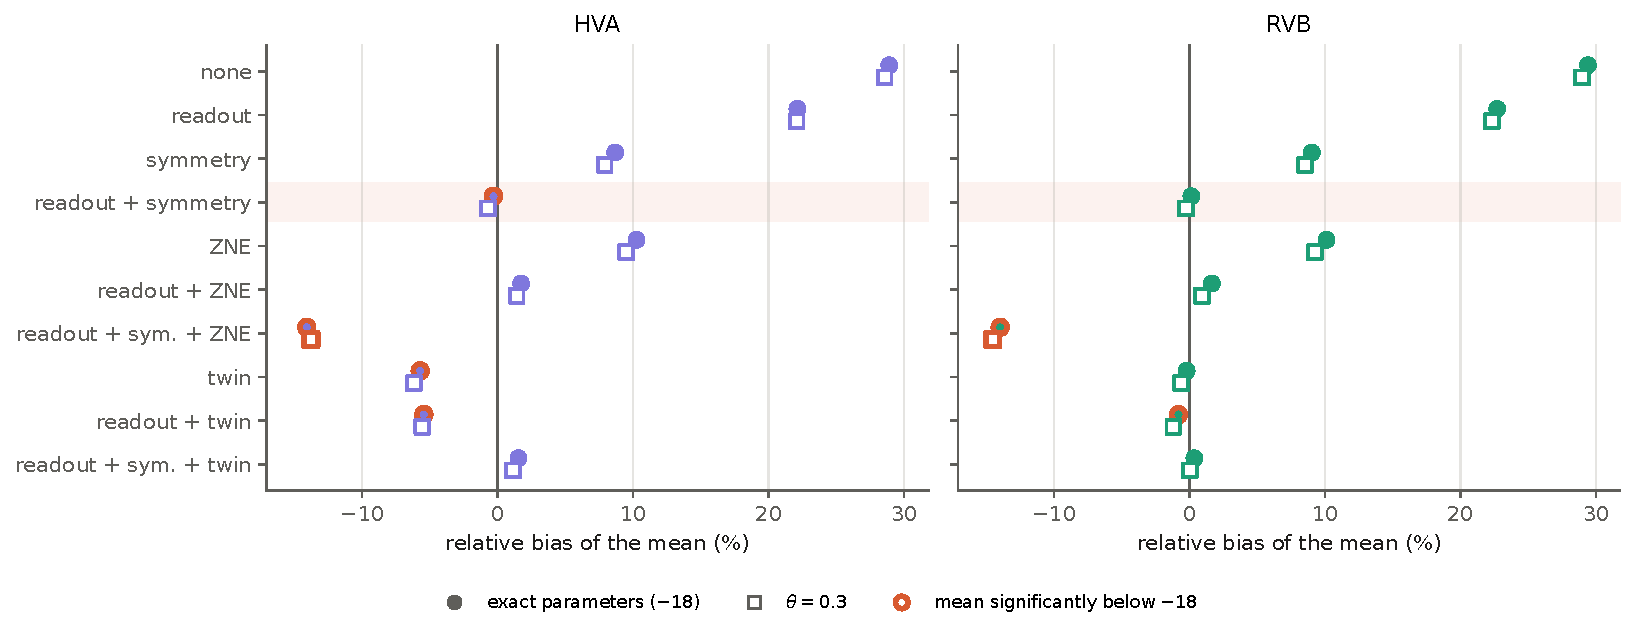
\includegraphics[width=\linewidth]{m2_stacks}
  \caption{The same data as Table~\ref{tab:m2}. Bars: $\pm2$ standard errors of the mean. The
    shaded row is the stack the development session chose. Stacks containing both symmetry and
    ZNE, and the twin stacks for HVA, land far below the noise-free value.}
  \label{fig:m2stacks}
\end{figure}

Figure~\ref{fig:m2stacks} sorts the stacks into three groups.
\begin{itemize}
  \item \textbf{Single techniques remove part of the bias.} Readout correction alone moves HVA at
    $\theta=0$ from \VMtHvaZeroRaw{} to \VMtHvaZeroRo, the readout factor of Table~\ref{tab:floor}.
    Symmetry alone reaches \VMtHvaZeroSym; ZNE alone \VMtHvaZeroZne{} at three times the shots.
  \item \textbf{Two combinations come close.} Readout + symmetry: \VMtHvaZeroRoSymRel{} (HVA) and
    \VMtRvbZeroRoSymRel{} (RVB) at $\theta=0$, \VMtHvaPtRoSymRel{} and \VMtRvbPtRoSymRel{} at
    $\theta=\VBoundTheta$, with no extra shots per energy. Readout + ZNE: \VMtHvaZeroRoZneRel{}
    and \VMtRvbZeroRoZneRel{}, for any ansatz but at three times the shots.
  \item \textbf{Three kinds of stack overshoot.} Symmetry + ZNE goes to \VMtHvaZeroRoSymZne{} (HVA) and \VMtRvbZeroRoSymZne{} (RVB); twin
    rescaling for HVA overshoots by \VMtHvaZeroTwinRel; and readout + symmetry itself is
    \VMtHvaZeroRoSymBelow{} standard errors below $-18$ for HVA at $\theta=0$.
\end{itemize}

\paragraph{Why HVA's twin fails.} HVA's twin is at $(5\pi/4,5\pi/4)$ with noise-free energy
\VMtTwinIdealHva{} and noisy energy \VMtTwinNoisyHva, a rescaling factor \VMtTwinFactorHva. The
target at $\theta=0$ is damped less ($\VMtHvaZeroRaw/{-18}$) than the twin, so the factor
over-corrects. RVB's twin (noise-free \VMtTwinIdealRvb, noisy \VMtTwinNoisyRvb, factor
\VMtTwinFactorRvb) happens to be damped like the target, and rescaling works. The development
session also notes that on the Clifford grid ($\pi/2$ steps) every HVA point is a ground state
or has zero energy, so no Clifford twin exists for HVA on this lattice.

\paragraph{Why symmetry and ZNE do not stack.} The development session's explanation:
post-selection removes noise in a way that is not multiplicative in $\lambda$ (the kept fraction
itself falls with $\lambda$), so the exponential fit extrapolates a curve that does not have the
assumed shape. The observed overshoot, \VMtHvaZeroRoSymZneRel{} at $\theta=0$, is consistent with
that, but this report has not checked the mechanism separately.

\subsection{Why readout plus symmetry looks accurate}
\label{sec:m2cancel}

The development session attributed the small overshoot of readout + symmetry to the calibration
describing all shots while being applied to the post-selected ones. To test that, and to measure
how large the effect is, this report computed the \emph{infinite-shot} value of every
counts-level estimator exactly: the transpiled circuit is simulated as a density matrix, the
outcome distribution of each basis is read without sampling, the device's readout channel is
applied analytically, and the estimators of \cref{dfn:counts} are evaluated on that distribution
(\py{docsgen.physics.mitigation_exact}). The same computation with the full noise model
reproduces the sampled means of Table~\ref{tab:m2} to within their spread (e.g.\ HVA, $\theta=0$:
\VMxHvaZeroFullRaw, \VMxHvaZeroFullRo, \VMxHvaZeroFullSym, \VMxHvaZeroFullRoSym).

\begin{prop}[Filtering then correcting over-corrects]\label{prop:overcorrect}
  Assume independent readout errors with $e_0^{(q)},e_1^{(q)}\le e$, no other noise, and a
  noise-free distribution supported on $|b|=n/2$. Then the filtered distribution is
  $p+O(e^2)$, and to leading order the filter-then-correct estimator returns
  \[
    E_{\mathrm{ro+sym}}=\sum_t c_t\,\langle P_t\rangle\prod_{q\in S_t}\frac{1}{1-e_0^{(q)}-e_1^{(q)}}
      \;+\;O\bigl(e^2,\ \max_q|e_0^{(q)}-e_1^{(q)}|\bigr),
  \]
  a multiplicative over-correction of each two-body term by about $1/(1-2e)^2$.
\end{prop}

\begin{proof}[Proof sketch]
  A single bit flip changes $|b|$ by one, so every read string of weight $n/2$ arises either from
  no flip, with probability $p(b)\prod_q(1-e^{(q)}_{b_q})$, or from at least two flips, with
  probability $O(e^2)$. The kept fraction is $\prod_q(1-e_{b_q}^{(q)})+O(e^2)$, and dividing
  gives $\tilde p=p+O(e^2)$. The filtered shots are therefore already almost free of readout
  error, but the estimator still applies $v_q$. Writing
  $v_q(b)=s(b)/(1-e_0^{(q)}-e_1^{(q)})+(e_0^{(q)}-e_1^{(q)})/(1-e_0^{(q)}-e_1^{(q)})$ and taking
  the product over a two-site support gives
  $\prod_{q\in S_t}s(b_q)\big/\prod_{q\in S_t}(1-e_0^{(q)}-e_1^{(q)})$ up to the stated
  corrections. Averaging over $\tilde p$ gives the formula.
\end{proof}

With the calibrated $e=\VMtReadoutErr$, the predicted factor $1/(1-2e)^2$ is \VMxOverPredicted.
The exact computation with readout noise only gives $E_{\mathrm{ro+sym}}/E_{\mathrm{sym}}=\VMxOverFactor$:
readout + symmetry returns \VMxHvaZeroRoRoSym{} (\VMxHvaZeroRoRoSymRel) at the exact HVA
parameters, where readout correction alone is exact (\VMxHvaZeroRoRo).

\begin{table}[H]
  \centering
  \small
  \begin{adjustbox}{max width=\linewidth}
    % Generated by `uv run python -m docsgen`; do not edit.
\begin{tabular}{lcccc}
\toprule
 & \multicolumn{2}{c}{HVA, $\theta=0$ ($-18$)} & \multicolumn{2}{c}{RVB, $\theta=\VBoundTheta$ (\VMtIdealRvbPt)} \\
\cmidrule(lr){2-3}\cmidrule(lr){4-5}
estimator & readout noise only & full noise & readout noise only & full noise \\
\midrule
none & \VMxHvaZeroRoRaw\,{\small(\VMxHvaZeroRoRawRel)} & \VMxHvaZeroFullRaw\,{\small(\VMxHvaZeroFullRawRel)} & \VMxRvbPtRoRaw\,{\small(\VMxRvbPtRoRawRel)} & \VMxRvbPtFullRaw\,{\small(\VMxRvbPtFullRawRel)} \\
readout & \VMxHvaZeroRoRo\,{\small(\VMxHvaZeroRoRoRel)} & \VMxHvaZeroFullRo\,{\small(\VMxHvaZeroFullRoRel)} & \VMxRvbPtRoRo\,{\small(\VMxRvbPtRoRoRel)} & \VMxRvbPtFullRo\,{\small(\VMxRvbPtFullRoRel)} \\
symmetry & \VMxHvaZeroRoSym\,{\small(\VMxHvaZeroRoSymRel)} & \VMxHvaZeroFullSym\,{\small(\VMxHvaZeroFullSymRel)} & \VMxRvbPtRoSym\,{\small(\VMxRvbPtRoSymRel)} & \VMxRvbPtFullSym\,{\small(\VMxRvbPtFullSymRel)} \\
readout + symmetry (as implemented) & \VMxHvaZeroRoRoSym\,{\small(\VMxHvaZeroRoRoSymRel)} & \VMxHvaZeroFullRoSym\,{\small(\VMxHvaZeroFullRoSymRel)} & \VMxRvbPtRoRoSym\,{\small(\VMxRvbPtRoRoSymRel)} & \VMxRvbPtFullRoSym\,{\small(\VMxRvbPtFullRoSymRel)} \\
correct, then filter (sector-aware) & \VMxHvaZeroRoCtf\,{\small(\VMxHvaZeroRoCtfRel)} & \VMxHvaZeroFullCtf\,{\small(\VMxHvaZeroFullCtfRel)} & \VMxRvbPtRoCtf\,{\small(\VMxRvbPtRoCtfRel)} & \VMxRvbPtFullCtf\,{\small(\VMxRvbPtFullCtfRel)} \\
\midrule
kept fraction (symmetry) & \VMxHvaZeroRoKept & \VMxHvaZeroFullKept & \VMxRvbPtRoKept & \VMxRvbPtFullKept \\
\bottomrule
\end{tabular}

  \end{adjustbox}
  \caption{Infinite-shot energy of each counts-level estimator, with the relative bias in
    brackets. Readout noise only: the device's readout channel and nothing else. Full noise: gate
    errors, $T_1/T_2$ and readout. ``Correct, then filter'' inverts the calibrated readout channel
    on the whole outcome distribution and then projects the resulting quasi-probabilities onto
    weight $n/2$.}
  \label{tab:m2exact}
\end{table}

\begin{figure}[H]
  \centering
  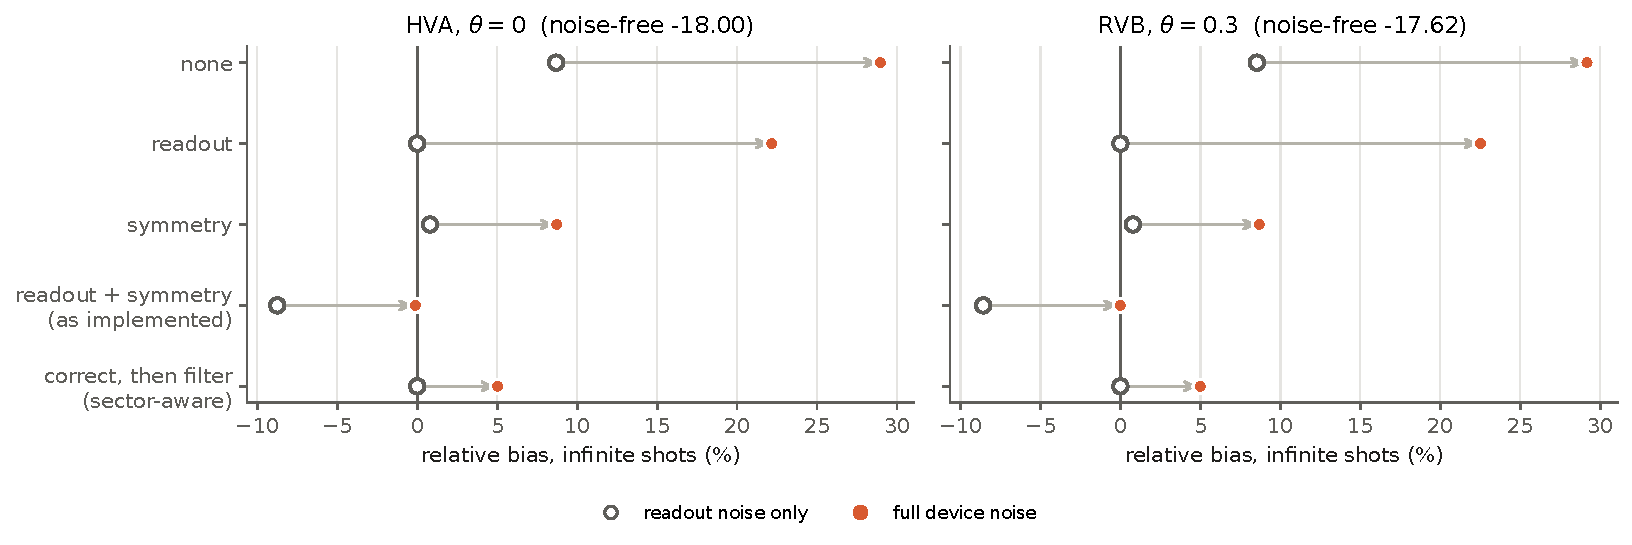
\includegraphics[width=\linewidth]{m2_exact}
  \caption{Each arrow goes from readout noise only (hollow) to full noise (filled). Readout +
    symmetry as implemented starts \emph{below} the noise-free value and is pushed back up by gate
    noise, ending near zero bias by cancellation. Correcting before filtering is exact under
    readout noise and leaves only the gate noise the filter cannot see.}
  \label{fig:m2exact}
\end{figure}

Table~\ref{tab:m2exact} and Figure~\ref{fig:m2exact} separate the two effects.
\begin{enumerate}
  \item \textbf{Readout noise alone} gives readout + symmetry an overshoot of
    \VMxHvaZeroRoRoSymRel{} (HVA, $\theta=0$) and \VMxRvbPtRoRoSymRel{} (RVB,
    $\theta=\VBoundTheta$), as \cref{prop:overcorrect} predicts.
  \item \textbf{Gate noise alone} leaves a bias that symmetry filtering cannot
    remove. The sector-aware estimator, which treats readout consistently, isolates it:
    \VMxHvaZeroFullCtfRel{} and \VMxRvbPtFullCtfRel.
  \item \textbf{Under full noise}, to leading order readout + symmetry equals the symmetry-only
    energy times the over-correction factor: $\VMxOverFactor\times\VMxHvaZeroFullSym=\VMxPredictFull$,
    against \VMxHvaZeroFullRoSym{} computed. The symmetry-only bias (\VMxHvaZeroFullSymRel) and the
    over-correction (\VMxOverPct) happen to be nearly equal on this device.
\end{enumerate}

\begin{rem}[Consequence]
  The small bias of the chosen stack is a property of \py{FakeGuadalupeV2}'s ratio of readout
  error to gate error, not of the method. On a device with relatively less gate noise, or after
  depth compression (M4) removes CX gates, the same stack will move further below the
  noise-free value. Readings below $-18$ in an optimisation are therefore expected, not
  accidental. The sector-aware estimator is principled but leaves \VMxHvaZeroFullCtfRel, and it works with
  quasi-probabilities, so its variance is larger; it was computed here only in the
  infinite-shot limit.
\end{rem}

\paragraph{Follow-up on \py{main}.} The development session reproduced both effects
independently, with sampled runs that switch on one error source at a time. It withdrew the
chosen stack and changed \py{CountsEnergy} to correct then filter when readout and symmetry
are both enabled (commit \texttt{56aadd3}). The new estimator inverts the tensored calibration on
the full $2^n$ outcome distribution and reports a bootstrap standard error, so it is limited to
20 qubits. A new \py{backend.noise} switch (\py{full}, \py{readout}, \py{gates}) makes the
single-source tables part of the benchmark. The reruns (\py{m2b-*}) will decide what to stack on
top of the corrected estimator to remove the remaining gate residual (\VMxHvaZeroFullCtfRel{} at the exact HVA parameters); this
chapter will be updated when they land.

\subsection{Full optimisations with the chosen stack}

\py{configs/m2_mitigated_vqe.toml} reran the M1 recommendations with readout + symmetry
(filter first, as in \texttt{c9272e3}) on the same noise: HVA with plain SPSA (\VMvItersHvaSpsa{} iterations) and RVB with ADAM and parameter
shift (\VMvItersRvbPs{} iterations, \VMvShotsPerRvbPs{} shots per basis).

\begin{table}[H]
  \centering
  \small
  \begin{adjustbox}{max width=\linewidth}
    % Generated by `uv run python -m docsgen`; do not edit.
\begin{tabular}{lcccccc}
\toprule
run & iterations & final energy (re-measured) & rel.\ error & $\sigma$ below $-18$ & noise-free energy of final params & total shots \\
\midrule
HVA, plain SPSA & \VMvItersHvaSpsa & \VMvFinalHvaSpsa ${}\pm{}$ \VMvStdHvaSpsa & \VMvErrHvaSpsa & \VMvBelowHvaSpsa & \VMvIdealHvaSpsa\,{\small(\VMvIdealErrHvaSpsa)} & \VMvShotsHvaSpsa \\
RVB, ADAM + parameter shift & \VMvItersRvbPs & \VMvFinalRvbPs ${}\pm{}$ \VMvStdRvbPs & \VMvErrRvbPs & -- & \VMvIdealRvbPs\,{\small(\VMvIdealErrRvbPs)} & \VMvShotsRvbPs \\
\bottomrule
\end{tabular}

  \end{adjustbox}
  \caption{Mitigated optimisations on \py{FakeGuadalupeV2} noise. The final energy is re-measured
    with 16384 shots per basis through the same stack. The noise-free energy of the final
    parameters (relative error in brackets) is computed classically and measures the
    parameters, independently of the estimator's bias.}
  \label{tab:m2vqe}
\end{table}

\begin{figure}[H]
  \centering
  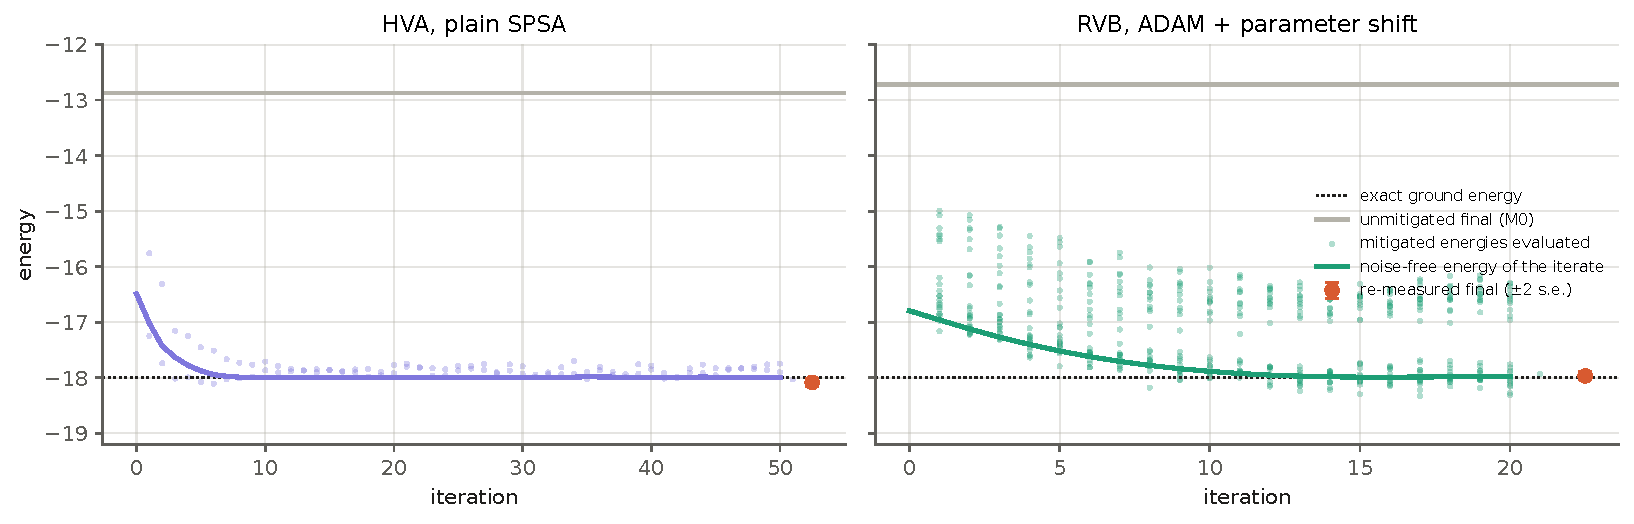
\includegraphics[width=\linewidth]{m2_vqe}
  \caption{Every mitigated energy evaluated (dots), the noise-free energy of the iterate (line),
    and the re-measured final value. Grey: the unmitigated final energy of the same combination
    after M0. ADAM with parameter shift evaluates shifted points, so its dots scatter above the
    iterate.}
  \label{fig:m2vqe}
\end{figure}

Both runs end with parameters whose noise-free energy is within \VMvIdealErrHvaSpsa{} (HVA) and
\VMvIdealErrRvbPs{} (RVB) of $-18$: the optimisers work under mitigation. The re-measured
energies differ from those noise-free values by the stack's bias. HVA reads \VMvFinalHvaSpsa{},
\VMvBelowHvaSpsa{} standard errors below $-18$, which by \cref{prop:mixed} is an artefact. This
is the over-correction of \cref{sec:m2cancel}, not a better state. The total cost is
\VMvShotsHvaSpsa{} and \VMvShotsRvbPs{} shots.

\subsection{Problems solved and open}

\begin{itemize}
  \item[\checkmark] Four mitigation layers, composable, on Aer and the IBM sampler; unit-tested.
    The counts layer reports exact standard errors.
  \item[\checkmark] Fixed-point evaluation mode with a below-ground flag: every stack's bias and
    cost measured at two points.
  \item[\checkmark] Mitigated optimisations reach parameters within \VMvIdealErrRvbPs{} (RVB) and
    \VMvIdealErrHvaSpsa{} (HVA) of the ground energy (noise-free); the estimates read
    \VMvFinalRvbPs{} and \VMvFinalHvaSpsa{} instead of about \VPostFinalRvbAdam.
  \item[$\circ$] \textbf{The chosen stack's accuracy was a cancellation} (\cref{sec:m2cancel});
    the stack is withdrawn. The sector-aware estimator is now on \py{main} (\texttt{56aadd3}).
    Still open: its finite-shot variance, and what removes the remaining gate residual of
    \VMxHvaZeroFullCtfRel{} (reruns pending).
  \item[$\circ$] \textbf{Symmetry and ZNE must not be stacked} as implemented.
  \item[$\circ$] \textbf{HVA has no usable twin}; rescaling is only as good as the twin's damping
    match.
  \item[$\circ$] \textbf{Hardware checks H0 and H1 are skipped}, so neither the noise floor nor
    the mitigation has been tested against a real device.
  \item[$\circ$] \textbf{The instance is easy} (\cref{rem:easy}): at $\theta=0$ the state is a
    singlet product, which symmetry filtering suits unusually well. The generic point confirms
    the trend, but M3 instances are needed before generalising.
\end{itemize}

\subsection*{Exercises}

\begin{exer}
  A qubit has $e_0=0.02$ and $e_1=0.03$. Compute $v(0)$ and $v(1)$, and check
  $\mathbb E[v(\tilde b)\mid b=1]=-1$.
\end{exer}
\begin{sol}
  $1-e_0-e_1=0.95$, so $v(0)=(1-0.03+0.02)/0.95=0.99/0.95\approx1.0421$ and
  $v(1)=-(1+0.03-0.02)/0.95=-1.01/0.95\approx-1.0632$. Given $b=1$, the read bit is $0$ with
  probability $e_1=0.03$, so the mean is $0.03\cdot1.0421+0.97\cdot(-1.0632)=0.03126-1.03126=-1.0000$.
\end{sol}

\begin{exer}
  Under readout noise only, why is symmetry filtering by itself \emph{not} exact
  (Table~\ref{tab:m2exact}: \VMxHvaZeroRoSymRel), although it removes every single-flip error?
\end{exer}
\begin{sol}
  Two flips in opposite directions ($0\to1$ on one qubit and $1\to0$ on another) keep the weight
  at $n/2$ and pass the filter. They occur with probability $O(e^2)$ per shot, but there are
  many qubit pairs: about $\binom{12}{2}\,e^2\approx66\times(0.022)^2\approx3\,\%$ of shots carry
  a double flip, a fraction of which pass. A pair flip inside a bond changes that bond's $Z_iZ_j$
  reading only if exactly one of its qubits flips, which biases the energy upward by a fraction
  of a percent.
\end{sol}

\begin{exer}
  Using the twin data of the HVA row, predict the twin-rescaled energy at $\theta=0$ from the raw
  mean, and compare with Table~\ref{tab:m2}.
\end{exer}
\begin{sol}
  $E_{\mathrm{mit}}=\VMtHvaZeroRaw\times\VMtTwinIdealHva/\VMtTwinNoisyHva=\VMtHvaZeroRaw\times\VMtTwinFactorHva\approx-19.0$,
  matching the twin row, \VMtHvaZeroTwin. The raw estimate and the twin come from separate runs,
  so the agreement is within the spread. The overshoot follows from the target being damped by
  $12.80/18\approx0.711$ and the twin by $7.56/11.25\approx0.672$.
\end{sol}

\section{Status, scorecard and open problems}
\label{sec:status}

\begin{table}[H]
  \centering
  \small
  \begin{tabular}{L{1.2cm}L{4.4cm}L{6.6cm}L{1.6cm}}
    \toprule
    & question & answer so far & status \\
    \midrule
    M0 & Are the noisy numbers real? & Not before M0. Floor now \VPostFinalMin{} to
      \VPostFinalMax{}; a bias, not a convergence failure (\cref{sec:noise}). & done \\
    M1 & Which gradient gives most precision per shot? & RVB: ADAM + parameter shift
      (\VMIdealRvbPs). HVA: plain SPSA (\VMIdealHvaSpsa). & done \\
    M2 & How much bias can mitigation remove? & -- & next \\
    M3 & Is the benchmark testing anything? & Not much: exact at zero parameters
      (\cref{thm:cycle}). & planned \\
    M4 & How far can depth fall? & Free first step found: bind parameters before
      transpiling, \VCxHva{} $\to$ \VBoundCxHva{} CX (\cref{prop:bound}). & planned \\
    M5 & Can subspace methods remove the rest? & -- & planned \\
    \bottomrule
  \end{tabular}
  \caption{Running scorecard, one row per roadmap milestone (\py{docs/roadmap.md}).}
  \label{tab:scorecard}
\end{table}

\subsection{Open problems}

\begin{enumerate}
  \item \textbf{The noisy floor} (\VFloorHvaFull{} at the exact parameters) is the dominant
    error, about \VPostErrHvaSpsa. Better optimisers cannot remove it (\cref{prop:mixed} and \cref{prop:depol}).
    The near-multiplicative structure of Table~\ref{tab:floor} favours rescaling and
    extrapolation \parencite{temme2017} (M2) and fewer CX (M4).
  \item \textbf{Hardware calibration H0} is deferred; every noisy number here is a simulation of
    a 2022 calibration snapshot.
  \item \textbf{M1 follow-ups:} decaying ADAM learning rate for HVA; longer RVB runs; more seeds
    with device noise.
  \item \textbf{The instance is easy} (\cref{rem:easy}); results should be re-validated on M3
    instances before conclusions generalise.
\end{enumerate}

\subsection{Issues found while writing this report}

These were found by recomputing every number from the code. The development session
reproduced each of them and is fixing the prose and code on \py{main}.
\begin{itemize}
  \item Parametric transpilation leaves each Heisenberg block at 5 CX instead of 3
    (\cref{prop:bound}). Binding first gives \VBoundCxHva{} CX and keeps \VBoundKeepHva{} instead of
    \VParamKeepHva{} of the energy at a generic point.
  \item \py{docs/physics.md} quotes 93 CX for RVB; the code gives \VCxRvb.
  \item The README's seed spreads were population standard deviations (Table~\ref{tab:m1},
    footnote); \py{main} is switching aggregated tables to sample standard deviations.
  \item The M0 spread figures and those in this report were measured under different conditions,
    and both are valid. The roadmap's figures (\VRoadmapSpreadLow{} at 1024 shots, \VRoadmapSpreadHigh{} at 4096) were taken
    \emph{with} \py{FakeGuadalupeV2} noise at the exact parameters, where noise breaks the
    cancellation of \cref{prop:zerovar}. This report's figures (\VSpreadLowReal, \VSpreadHighReal)
    are noise-free at the start point. Without noise the spread at the optimum is exactly zero,
    so the roadmap now states the conditions of its measurement.
  \item \py{HVAnsatz}'s docstring writes $e^{-i\gamma\Hev}e^{-i\phi\Hod}$; the circuit implements
    $e^{-i\frac\gamma2\Hev}e^{-i\frac\phi2\Hod}$ (\cref{dfn:ansatz}). Only the convention differs.
\end{itemize}


\printbibliography

\appendix
\section{Reproducing this report}
\label{app:reproduce}

All figures, tables and quoted numbers come from \py{docsgen/}, a small package at the repository
root that reads \py{results/} and calls \py{kagome_vqe}. Nothing in the \LaTeX{} sources types a
measured value by hand: every number is a \verb|\V<key>| macro defined in
\py{report/tables/numbers.tex}, whose comments name the source of each value.

\begin{center}
\begin{tabular}{L{6.2cm}L{8.8cm}}
  \toprule
  command & effect \\
  \midrule
  \py{uv run python -m docsgen} & regenerate numbers, tables, figures and slide data \\
  \py{uv run python -m docsgen --recompute} & also rerun the cached simulator studies (about a minute) \\
  \py{uv run pytest docsgen/tests} & assert every quoted number against code and results \\
  \py{just report} & build this PDF with \py{latexmk} (XeLaTeX, biber) into \py{report/output/} \\
  \py{just slides-serve} & serve the reveal.js deck on \py{http://localhost:8000} \\
  \bottomrule
\end{tabular}
\end{center}

Five numbers are quoted from \py{docs/roadmap.md} rather than recomputed: the spread, row count
and fake gradient of the pre-M0 seed bug (\cref{sec:m0}), whose code was replaced, and the
roadmap's two noisy spread figures (\cref{sec:status}), which are cited for comparison.
The test suite checks that no other number is quoted. Simulator studies use the fixed seed
$20261010$, so a recompute reproduces the cache.


\end{document}
